\documentclass[semcabeco,showtrims,10pt,conselho,spreadimages]{memoir}

\usepackage[catalogo2]{hedraoptions} %% << %%%%%%%%%%%%%%%%
\usepackage[baruch]{hedrastyles}
\usepackage[xetex,chicagofootnotes]{tipografia}
\usepackage[standart,sempontinhos]{toc}
\usepackage{hedraextra}
\usepackage{penalidades}
\usepackage{graficos}
\usepackage{hedralogo}
\usepackage{hifensextras}
\usepackage{fichatecnica}
\usepackage[standart]{aparatos}
\usepackage{tabelas}
\usepackage{versos}
\usepackage{gitrevisioninfo}

\usepackage{wasysym}
\usepackage{amssymb}

\usepackage{wrapfig}



\newcommand{\forceindent}{\leavevmode{\parindent=1em\indent}}


\linespread{1.15}

\usepackage{endnotes}
\renewcommand{\notesname}{Notas}

\usepackage{multicol}

%\counterwithin*{endnote}{part}
%\counterwithin*{endnote}{chapter}

%\let\latexchapter\chapter
%\makeatletter
%\renewcommand\enoteheading{%
  %\setcounter{secnumdepth}{-2}
  %\latexchapter*{\notesname\markboth{NOTAS}{}}
  %\mbox{}\par\vskip-\baselineskip
  %\let\@afterindentfalse\@afterindenttrue
%}
%\makeatother

\baselineskip=15pt


\usepackage{xcolor, soul}

\newcommand{\hlc}[2][yellow]{{\sethlcolor{#1}\hl{#2}}}
\colorlet{lightyellow}{yellow!60}


\usepackage{hyphenat}


%--------------------------------------------PERMITIR FONTES MAIORES (HUGE)

\usepackage{anyfontsize}

%--------------------------------------------TIRAR TRAÇO DIVISOR DA FOOTNOTE

\usepackage{footmisc}

\renewcommand*\footnoterule{}
%\fancyhf[RO]{\cnvt{\thepage} -- \thepage}
%\fancyfoot{}
%\renewcommand{\headrulewidth}{0pt}
%\renewcommand{\footrulewidth}{0pt}}

%--------------------------------------------DEFININDO FONTES A SEREM USADAS NO LIVRO

\usepackage{fontspec}

%\setmainfont[Ligatures=TeX]{Formular-Regular}

\newcommand{\slsc}[1]{\fontspec[SmallCapsFeatures={FakeSlant=0.6}]{Formular-LightItalic}\textsc{#1}\fontspec[]{FormularLight-Italic}}

%\usepackage{Formular}
\setmainfont{Formular-Regular.otf}[
BoldFont = Formular-Bold.otf ,
ItalicFont = Formular-Italic.otf]

\newfontfamily\fakereceipt{fakereceipt}
\newfontfamily\arial{arial}
%\newfontfamily\Cobraarisca{Cobra arisca-Regular}
%\newfontfamily\fakereceipt{fake receipt}
%\newfontfamily\Brabo{FS Brabo Pro-Regular}

%--------------------------------------------ALTERAR FONTE DA NOTA DE RODAPÉ

%\setsansfont{Formular-Light}


\usepackage{etoolbox}
\makeatletter
\patchcmd{\@footnotetext}{\footnotesize}{\scriptsize\sffamily}{}{}
\makeatother


%--------------------------------------------ALTERAR FONTE DA NUMERAÇÃO DE PÁGINA
\usepackage{graphicx}
\usepackage{fancyhdr}
\fancyhfoffset[]{3cm}
\pagestyle{fancy}
\fancyhf{}
\rhead{Catálogo EdLab \hspace{2cm}}
\lhead{\hspace{2cm} \thepage \hspace{.25cm} \textbf{Livros}}


%\fancyfoot[CE,CO]{\Formular \footnotesize \textit \thepage}%\renewcommand{\headrulewidth}{0pt}

\usepackage{titlesec}

\titleformat{\chapter}
[display]
{\Large\bfseries}
 {\large\chaptertitlename\space\thechapter}
  {20pt}
  {\flushleft}


%%% HEADERS DE CADA EDITORA

\fancypagestyle{grid}{
\setlength{\headsep}{1cm}
\fancyhf{}
\fancyhead[RE]{Catálogo EdLab \hspace{2cm}}
\fancyhead[LE]{\rule[-1ex]{0pt}{1ex} \hspace{2cm} \thepage \hspace{.25cm} \textbf{Livros}}
\fancyhead[RO]{\rule[-1ex]{0pt}{1ex} \textbf{Livros} \hspace{.25cm} \thepage \hspace{2cm}}
\fancyhead[LO]{\rule[-1ex]{0pt}{1ex}  \hspace{2cm} Catálogo EdLab}
\fancyfoot[C]{}
}


\fancypagestyle{indice}{
\setlength{\headsep}{1cm}
\fancyhf{}
\fancyhead[L]{\rule[-1ex]{0pt}{1ex} \hspace{2cm} \textbf{Catálogo 2020/ 4}}
\fancyfoot[C]{}
}

\fancypagestyle{ayllon}{
\setlength{\headsep}{1cm}
\fancyhf{}
\fancyhead[RE]{\rule[-1ex]{0pt}{1ex} Catálogo EdLab \hspace{2cm}}
\fancyhead[LE]{\rule[-1ex]{0pt}{1ex} \hspace{2cm} \thepage \hspace{.25cm} \textbf{Aylllon}}
\fancyhead[RO]{\rule[-1ex]{0pt}{1ex} \textbf{Ayllon} \hspace{.25cm} \thepage \hspace{2cm}}
\fancyhead[LO]{\rule[-1ex]{0pt}{1ex}  \hspace{2cm} Catálogo EdLab}
\fancyfoot[C]{}
}

\fancypagestyle{azougue}{
\setlength{\headsep}{1cm}
\fancyhf{}
\fancyhead[RE]{\rule[-1ex]{0pt}{1ex} Catálogo EdLab \hspace{2cm}}
\fancyhead[LE]{\rule[-1ex]{0pt}{1ex} \hspace{2cm} \thepage \hspace{.25cm} \textbf{Azougue}}
\fancyhead[RO]{\rule[-1ex]{0pt}{1ex} \textbf{Azougue} \hspace{.25cm} \thepage \hspace{2cm}}
\fancyhead[LO]{\rule[-1ex]{0pt}{1ex}  \hspace{2cm} Catálogo EdLab}
\fancyfoot[C]{}
}

\fancypagestyle{azouguecat}{
\setlength{\headsep}{.5cm}
\fancyhf{}
\fancyhead[RE]{Livros ativos \hspace{2cm}}
\fancyhead[LE]{\rule[-1ex]{0pt}{1ex} \hspace{2cm} \thepage \hspace{.25cm} \textbf{Azougue}}
\fancyhead[RO]{\rule[-1ex]{0pt}{1ex} \textbf{Azougue} \hspace{.25cm} \thepage \hspace{2cm}}
\fancyhead[LO]{\rule[-1ex]{0pt}{1ex}  \hspace{2cm} Livros ativos}
\fancyfoot[C]{}
}

\fancypagestyle{circuito}{
\setlength{\headsep}{1cm}
\fancyhf{}
\fancyhead[RE]{\rule[-1ex]{0pt}{1ex} Catálogo EdLab \hspace{2cm}}
\fancyhead[LE]{\rule[-1ex]{0pt}{1ex} \hspace{2cm} \thepage \hspace{.25cm} \textbf{Circuito}}
\fancyhead[RO]{\rule[-1ex]{0pt}{1ex} \textbf{Circuito} \hspace{.25cm} \thepage \hspace{2cm}}
\fancyhead[LO]{\rule[-1ex]{0pt}{1ex}  \hspace{2cm} Catálogo EdLab}
\fancyfoot[C]{}
}

\fancypagestyle{circuitocat}{
\setlength{\headsep}{.5cm}
\fancyhf{}
\fancyhead[RE]{Livros ativos \hspace{2cm}}
\fancyhead[LE]{\rule[-1ex]{0pt}{1ex} \hspace{2cm} \thepage \hspace{.25cm} \textbf{Circuito}}
\fancyhead[RO]{\rule[-1ex]{0pt}{1ex} \textbf{Circuito} \hspace{.25cm} \thepage \hspace{2cm}}
\fancyhead[LO]{\rule[-1ex]{0pt}{1ex}  \hspace{2cm} Livros ativos}
\fancyfoot[C]{}
}

\fancypagestyle{hedra}{
\setlength{\headsep}{1cm}
\fancyhf{}
\fancyhead[RE]{\rule[-1ex]{0pt}{1ex} Catálogo EdLab \hspace{2cm}}
\fancyhead[LE]{\rule[-1ex]{0pt}{1ex} \hspace{2cm} \thepage \hspace{.25cm} \textbf{Hedra}}
\fancyhead[RO]{\rule[-1ex]{0pt}{1ex} \textbf{Hedra} \hspace{.25cm} \thepage \hspace{2cm}}
\fancyhead[LO]{\rule[-1ex]{0pt}{1ex}  \hspace{2cm} Catálogo EdLab}
\fancyfoot[C]{}
}

\fancypagestyle{hedracat}{
\setlength{\headsep}{.5cm}
\fancyhf{}
\fancyhead[RE]{Livros ativos \hspace{2cm}}
\fancyhead[LE]{\rule[-1ex]{0pt}{1ex} \hspace{2cm} \thepage \hspace{.25cm} \textbf{Hedra}}
\fancyhead[RO]{\rule[-1ex]{0pt}{1ex} \textbf{Hedra} \hspace{.25cm} \thepage \hspace{2cm}}
\fancyhead[LO]{\rule[-1ex]{0pt}{1ex}  \hspace{2cm} Livros ativos}
\fancyfoot[C]{}
}

\fancypagestyle{ima}{
\setlength{\headsep}{1cm}
\fancyhf{}
\fancyhead[RE]{\rule[-1ex]{0pt}{1ex} Catálogo EdLab \hspace{2cm}}
\fancyhead[LE]{\rule[-1ex]{0pt}{1ex} \hspace{2cm} \thepage \hspace{.25cm} \textbf{Ímã Editorial}}
\fancyhead[RO]{\rule[-1ex]{0pt}{1ex} \textbf{Ímã Editorial} \hspace{.25cm} \thepage \hspace{2cm}}
\fancyhead[LO]{\rule[-1ex]{0pt}{1ex}  \hspace{2cm} Catálogo EdLab}
\fancyfoot[C]{}
}

\fancypagestyle{imacat}{
\setlength{\headsep}{.5cm}
\fancyhf{}
\fancyhead[RE]{Livros ativos \hspace{2cm}}
\fancyhead[LE]{\rule[-1ex]{0pt}{1ex} \hspace{2cm} \thepage \hspace{.25cm} \textbf{Ímã Editorial}}
\fancyhead[RO]{\rule[-1ex]{0pt}{1ex} \textbf{Ímã Editorial} \hspace{.25cm} \thepage \hspace{2cm}}
\fancyhead[LO]{\rule[-1ex]{0pt}{1ex}  \hspace{2cm} Livros ativos}
\fancyfoot[C]{}
}

\fancypagestyle{kalinka}{
\setlength{\headsep}{1cm}
\fancyhf{}
\fancyhead[RE]{\rule[-1ex]{0pt}{1ex} Catálogo EdLab \hspace{2cm}}
\fancyhead[LE]{\rule[-1ex]{0pt}{1ex} \hspace{2cm} \thepage \hspace{.25cm} \textbf{Kalinka}}
\fancyhead[RO]{\rule[-1ex]{0pt}{1ex} \textbf{Kalinka} \hspace{.25cm} \thepage \hspace{2cm}}
\fancyhead[LO]{\rule[-1ex]{0pt}{1ex}  \hspace{2cm} Catálogo EdLab}
\fancyfoot[C]{}
}

\fancypagestyle{kalinkacat}{
\setlength{\headsep}{.5cm}
\fancyhf{}
\fancyhead[RE]{Livros ativos \hspace{2cm}}
\fancyhead[LE]{\rule[-1ex]{0pt}{1ex} \hspace{2cm} \thepage \hspace{.25cm} \textbf{Kalinka}}
\fancyhead[RO]{\rule[-1ex]{0pt}{1ex} \textbf{Kalinka} \hspace{.25cm} \thepage \hspace{2cm}}
\fancyhead[LO]{\rule[-1ex]{0pt}{1ex}  \hspace{2cm} Livros ativos}
\fancyfoot[C]{}
}

\fancypagestyle{n-1}{
\setlength{\headsep}{1cm}
\fancyhf{}
\fancyhead[R]{\rule[-1ex]{0pt}{1ex} Catálogo EdLab \hspace{2cm}}
\fancyhead[L]{\rule[-1ex]{0pt}{1ex} \hspace{2cm} \thepage \hspace{.25cm} \textbf{n-1 edições}}
\fancyhead[RO]{\rule[-1ex]{0pt}{1ex} \textbf{n-1 edições} \hspace{.25cm} \thepage \hspace{2cm}}
\fancyhead[LO]{\rule[-1ex]{0pt}{1ex}  \hspace{2cm} Catálogo EdLab}
\fancyfoot[C]{}
}

\fancypagestyle{n-1cat}{
\setlength{\headsep}{.5cm}
\fancyhf{}
\fancyhead[RE]{Livros ativos \hspace{2cm}}
\fancyhead[LE]{\rule[-1ex]{0pt}{1ex} \hspace{2cm} \thepage \hspace{.25cm} \textbf{n-1 edições}}
\fancyhead[RO]{\rule[-1ex]{0pt}{1ex} \textbf{n-1 edições} \hspace{.25cm} \thepage \hspace{2cm}}
\fancyhead[LO]{\rule[-1ex]{0pt}{1ex}  \hspace{2cm} Livros ativos}
\fancyfoot[C]{}
}

\fancypagestyle{quadrado}{
\setlength{\headsep}{1cm}
\fancyhf{}
\fancyhead[RE]{\rule[-1ex]{0pt}{1ex} Catálogo EdLab \hspace{2cm}}
\fancyhead[LE]{\rule[-1ex]{0pt}{1ex} \hspace{2cm} \thepage \hspace{.25cm} \textbf{Quadradocirculo}}
\fancyhead[RO]{\rule[-1ex]{0pt}{1ex} \textbf{Quadradocirculo} \hspace{.25cm} \thepage \hspace{2cm}}
\fancyhead[LO]{\rule[-1ex]{0pt}{1ex}  \hspace{2cm} Catálogo EdLab}
\fancyfoot[C]{}
}
%--------------------------------------------
\usepackage{afterpage}

\newcommand\blankpage{%
    \null
    \thispagestyle{empty}%
    \addtocounter{page}{0}%
    \newpage}


\newenvironment{changemargin}{
  \addtolength{\textheight}{-5mm}
  \addtolength{\headsep}{.7cm}
}


\usepackage{changepage}
\usepackage{placeins}
\usepackage{float}
\usepackage{floatpag}
\usepackage{rotating}
%\usepackage{afterpage}
\usepackage{paracol}
\setlength{\columnsep}{0.8cm}

\newenvironment{absolutelynopagebreak}
  {\par\nobreak\vfil\penalty0\vfilneg
   \vtop\bgroup}
  {\par\xdef\tpd{\the\prevdepth}\egroup
   \prevdepth=\tpd}


\setcounter{tocdepth}{0}
\setcounter{secnumdepth}{-2} 
%\linespread{1.08}

\makeatletter
\newenvironment{Parskip}{%
   \par
   \parskip=0.3\baselineskip \advance\parskip by 0pt plus 2pt
   \parindent=\z@
   \def\@listI{\leftmargin\leftmargini
      \topsep\z@ \parsep\parskip \itemsep\z@}
   \let\@listi\@listI
   \@listi
   \def\@listii{\leftmargin\leftmarginii
      \labelwidth\leftmarginii\advance\labelwidth-\labelsep
      \topsep\z@ \parsep\parskip \itemsep\z@}
   \def\@listiii{\leftmargin\leftmarginiii
       \labelwidth\leftmarginiii\advance\labelwidth-\labelsep
       \topsep\z@ \parsep\parskip \itemsep\z@}
   \partopsep=\z@
}{\par}
\makeatother

\makeatletter
\newenvironment{myParskip}{%
   \par
   \parskip=0.2\baselineskip \advance\parskip by 0pt plus 2pt
   \parindent=\z@
   \def\@listI{\leftmargin\leftmargini
      \topsep\z@ \parsep\parskip \itemsep\z@}
   \let\@listi\@listI
   \@listi
   \def\@listii{\leftmargin\leftmarginii
      \labelwidth\leftmarginii\advance\labelwidth-\labelsep
      \topsep\z@ \parsep\parskip \itemsep\z@}
   \def\@listiii{\leftmargin\leftmarginiii
       \labelwidth\leftmarginiii\advance\labelwidth-\labelsep
       \topsep\z@ \parsep\parskip \itemsep\z@}
   \partopsep=\z@
}{\par}
\makeatother

\newcommand{\mystar}{{\fontfamily{lmr}\selectfont$\star$}}


\begin{document}

%\input{ABRE}
\begin{textblock*}{5.625in}(0pt,0pt)%
\vspace*{-3cm}
%\hspace*{-2.1cm}\includegraphics*[width=162mm]{EDLAB}
\end{textblock*}

\pagebreak

\pagestyle{indice}

%{\centering{\includegraphics[width=130mm]{lettering.pdf}}}
\begin{center}
\newfontfamily\timesnewroman{Times New Roman}
{\fontsize{160}{50}\selectfont \timesnewroman hedra}
\end{center}
\vspace{1.2cm}

%\begingroup\raggedleft
%{\LARGE

%\hspace*{6.8cm}0\pageref{hedra} \textbf{SELEÇÃO ESPECIAL}

% \hspace*{6.8cm}\pageref{n-1} \textbf{N-1 EDIÇÕES}

% \hspace*{6.8cm}\pageref{circuito} \textbf{CIRCUITO}

% \hspace*{6.8cm}\pageref{ima} \textbf{ÍMÃ EDITORIAL}

% %\hspace*{6.8cm}\pageref{azougue} \textbf{AZOUGUE}

% \hspace*{6.8cm}\pageref{kalinka} \textbf{KALINKA}

% \hspace*{6.8cm}\pageref{ayllon} \textbf{AYLLON}\\

%\hspace*{6.5cm}\pageref{quadrado} \textbf{QUADRADOCIRCULO}\\}

%\endgroup

\hspace*{-7cm}\hrulefill\hspace*{-7cm}

\vspace{1cm}

\hspace*{-.5cm}\parbox{180pt}{\raggedright
Neste catálogo apresentamos 15
livros publicados pela editora Hedra, com temáticas voltadas 
para escolas e educação em geral. 

\vspace{1em}

Além dos livros selecionados, disponibilizamos ao final 
do catálogo uma lista completa de publicações ativas da editora. Lembramos aos 
livreiros que todos os nossos títulos
estão cadastrados na Metabooks.

\vspace{1em}

Conheça também nosso site

\textbf{hedra.com.br}
} %\enlargethispage{\baselineskip}

%\pagebreak
%\blankpage
\pagebreak

\pagestyle{grid}

\begin{figure}[!htbp]
\begin{tabular}{cccc}

\vspace{.5cm}
\hspace*{.5cm}
\subfloat{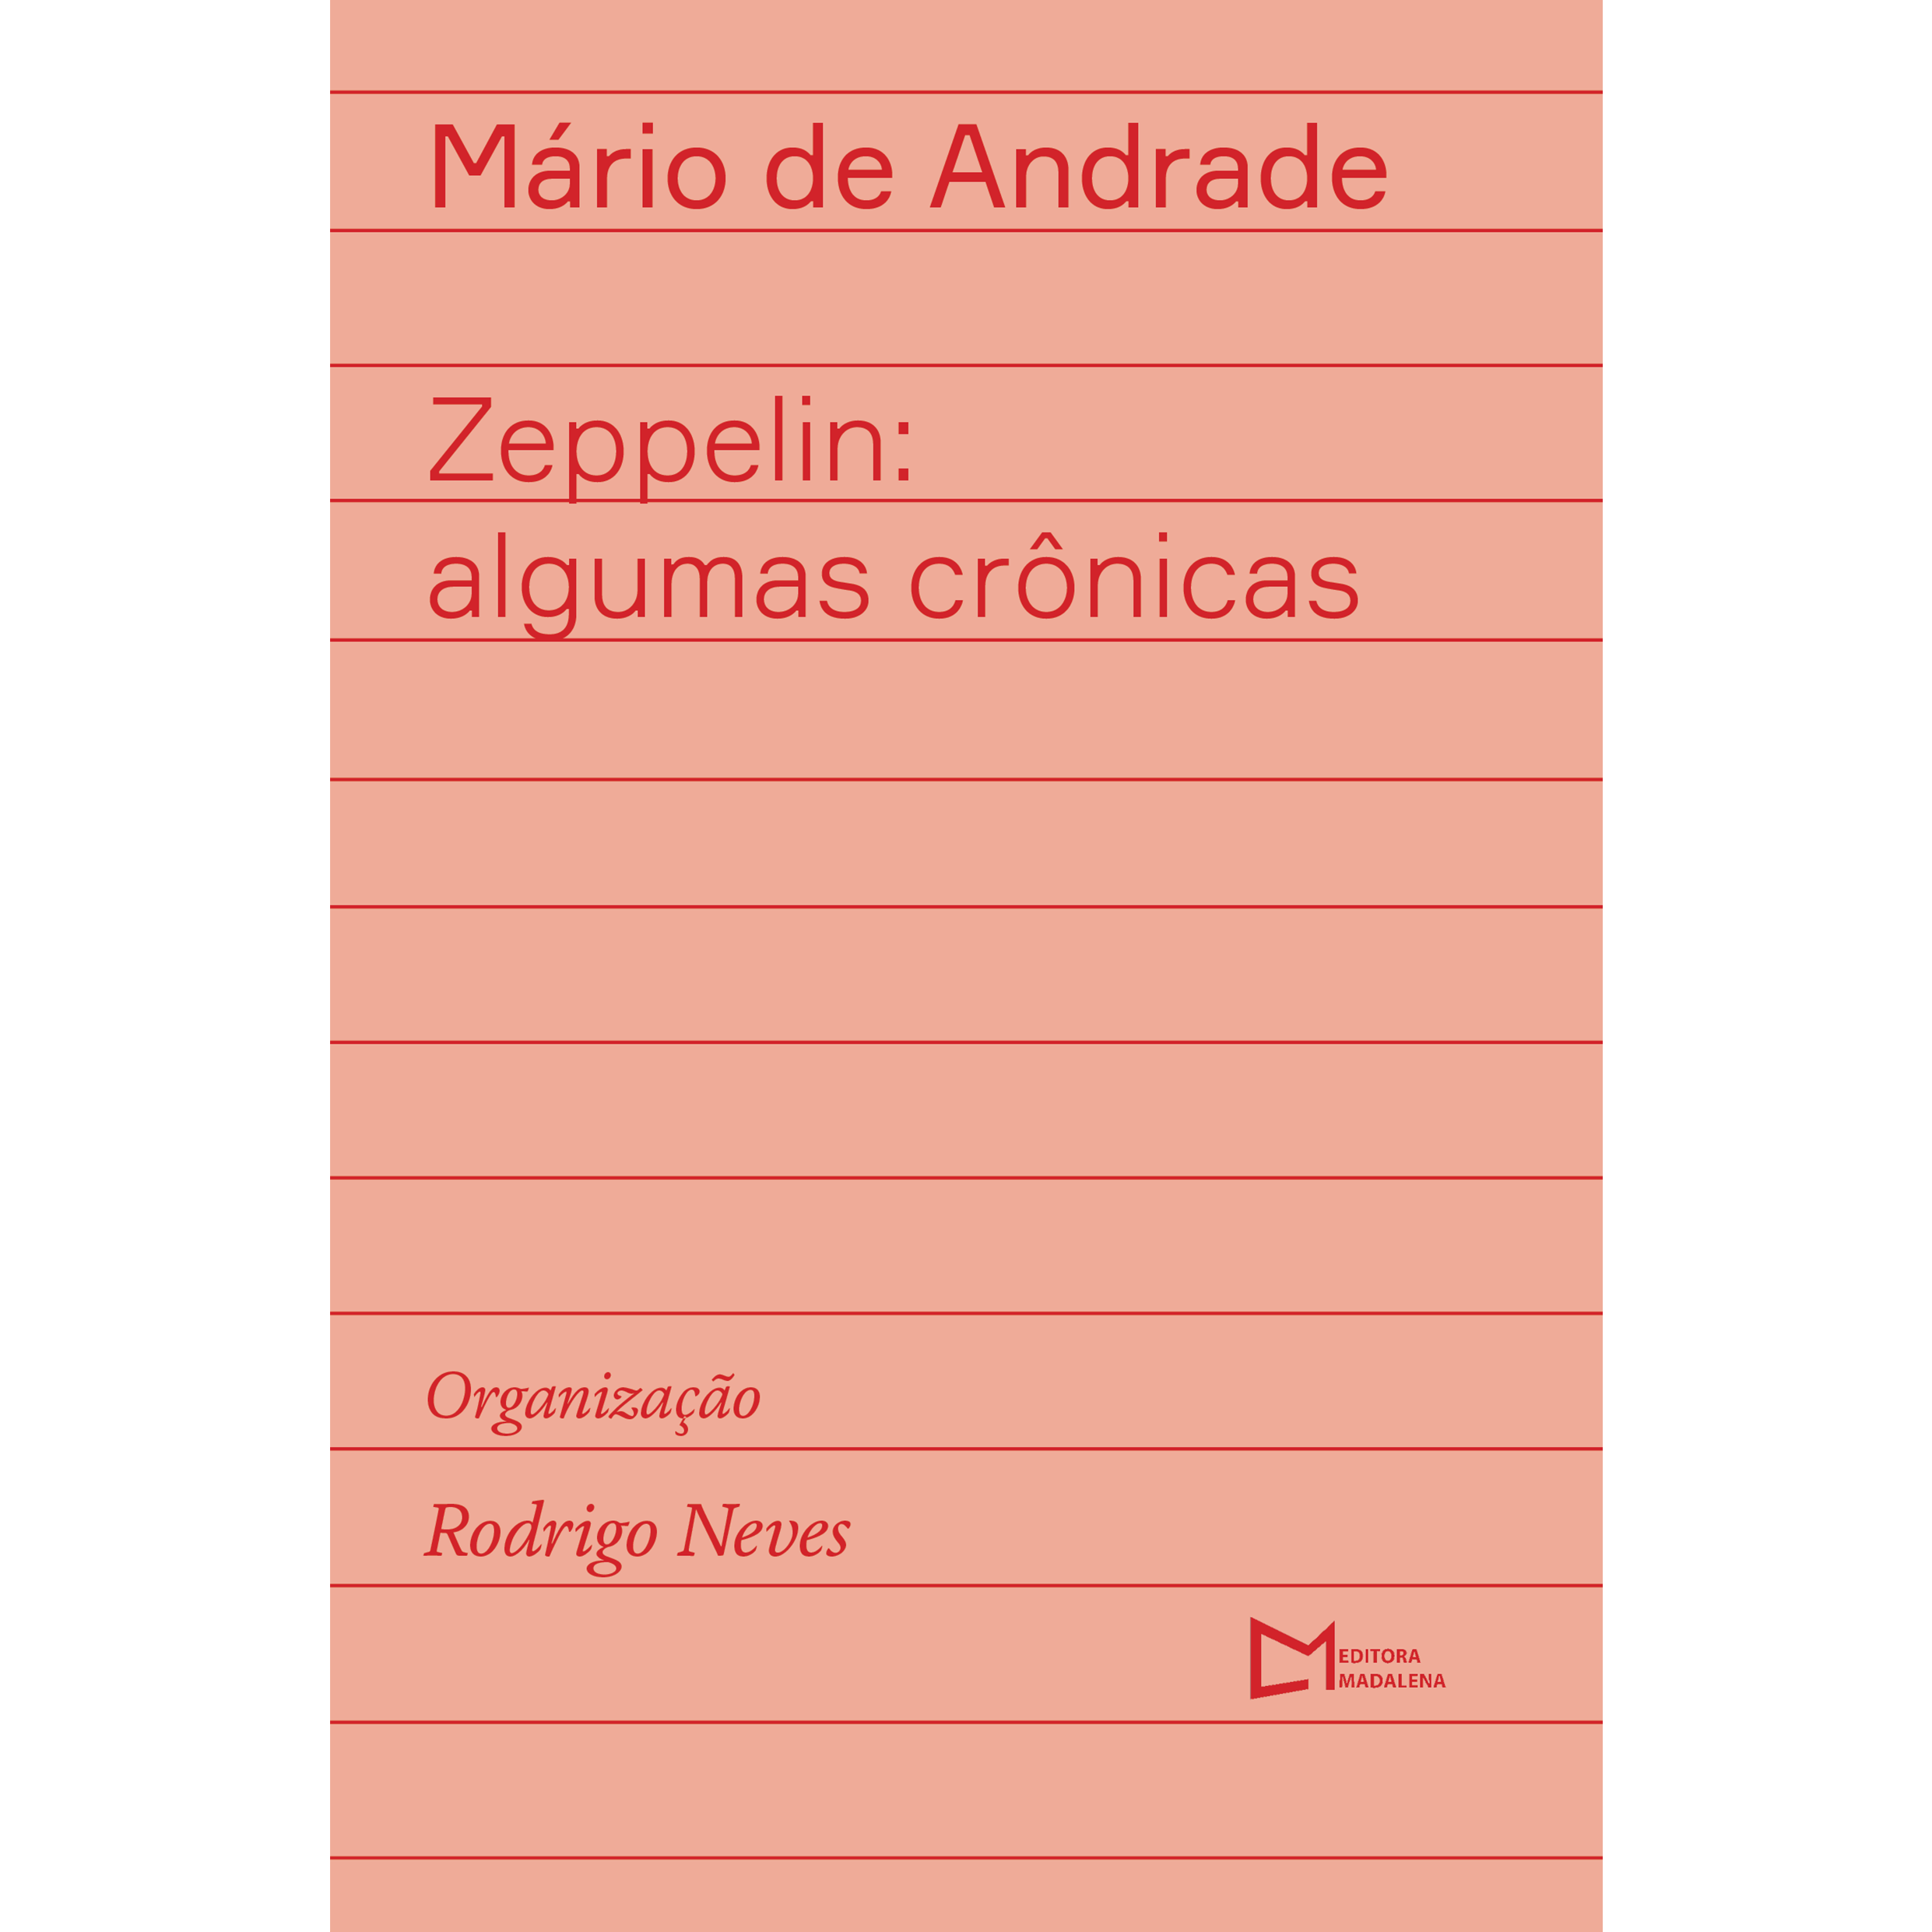
\includegraphics[width=40mm]{./grid/zepelin.png}}
\subfloat{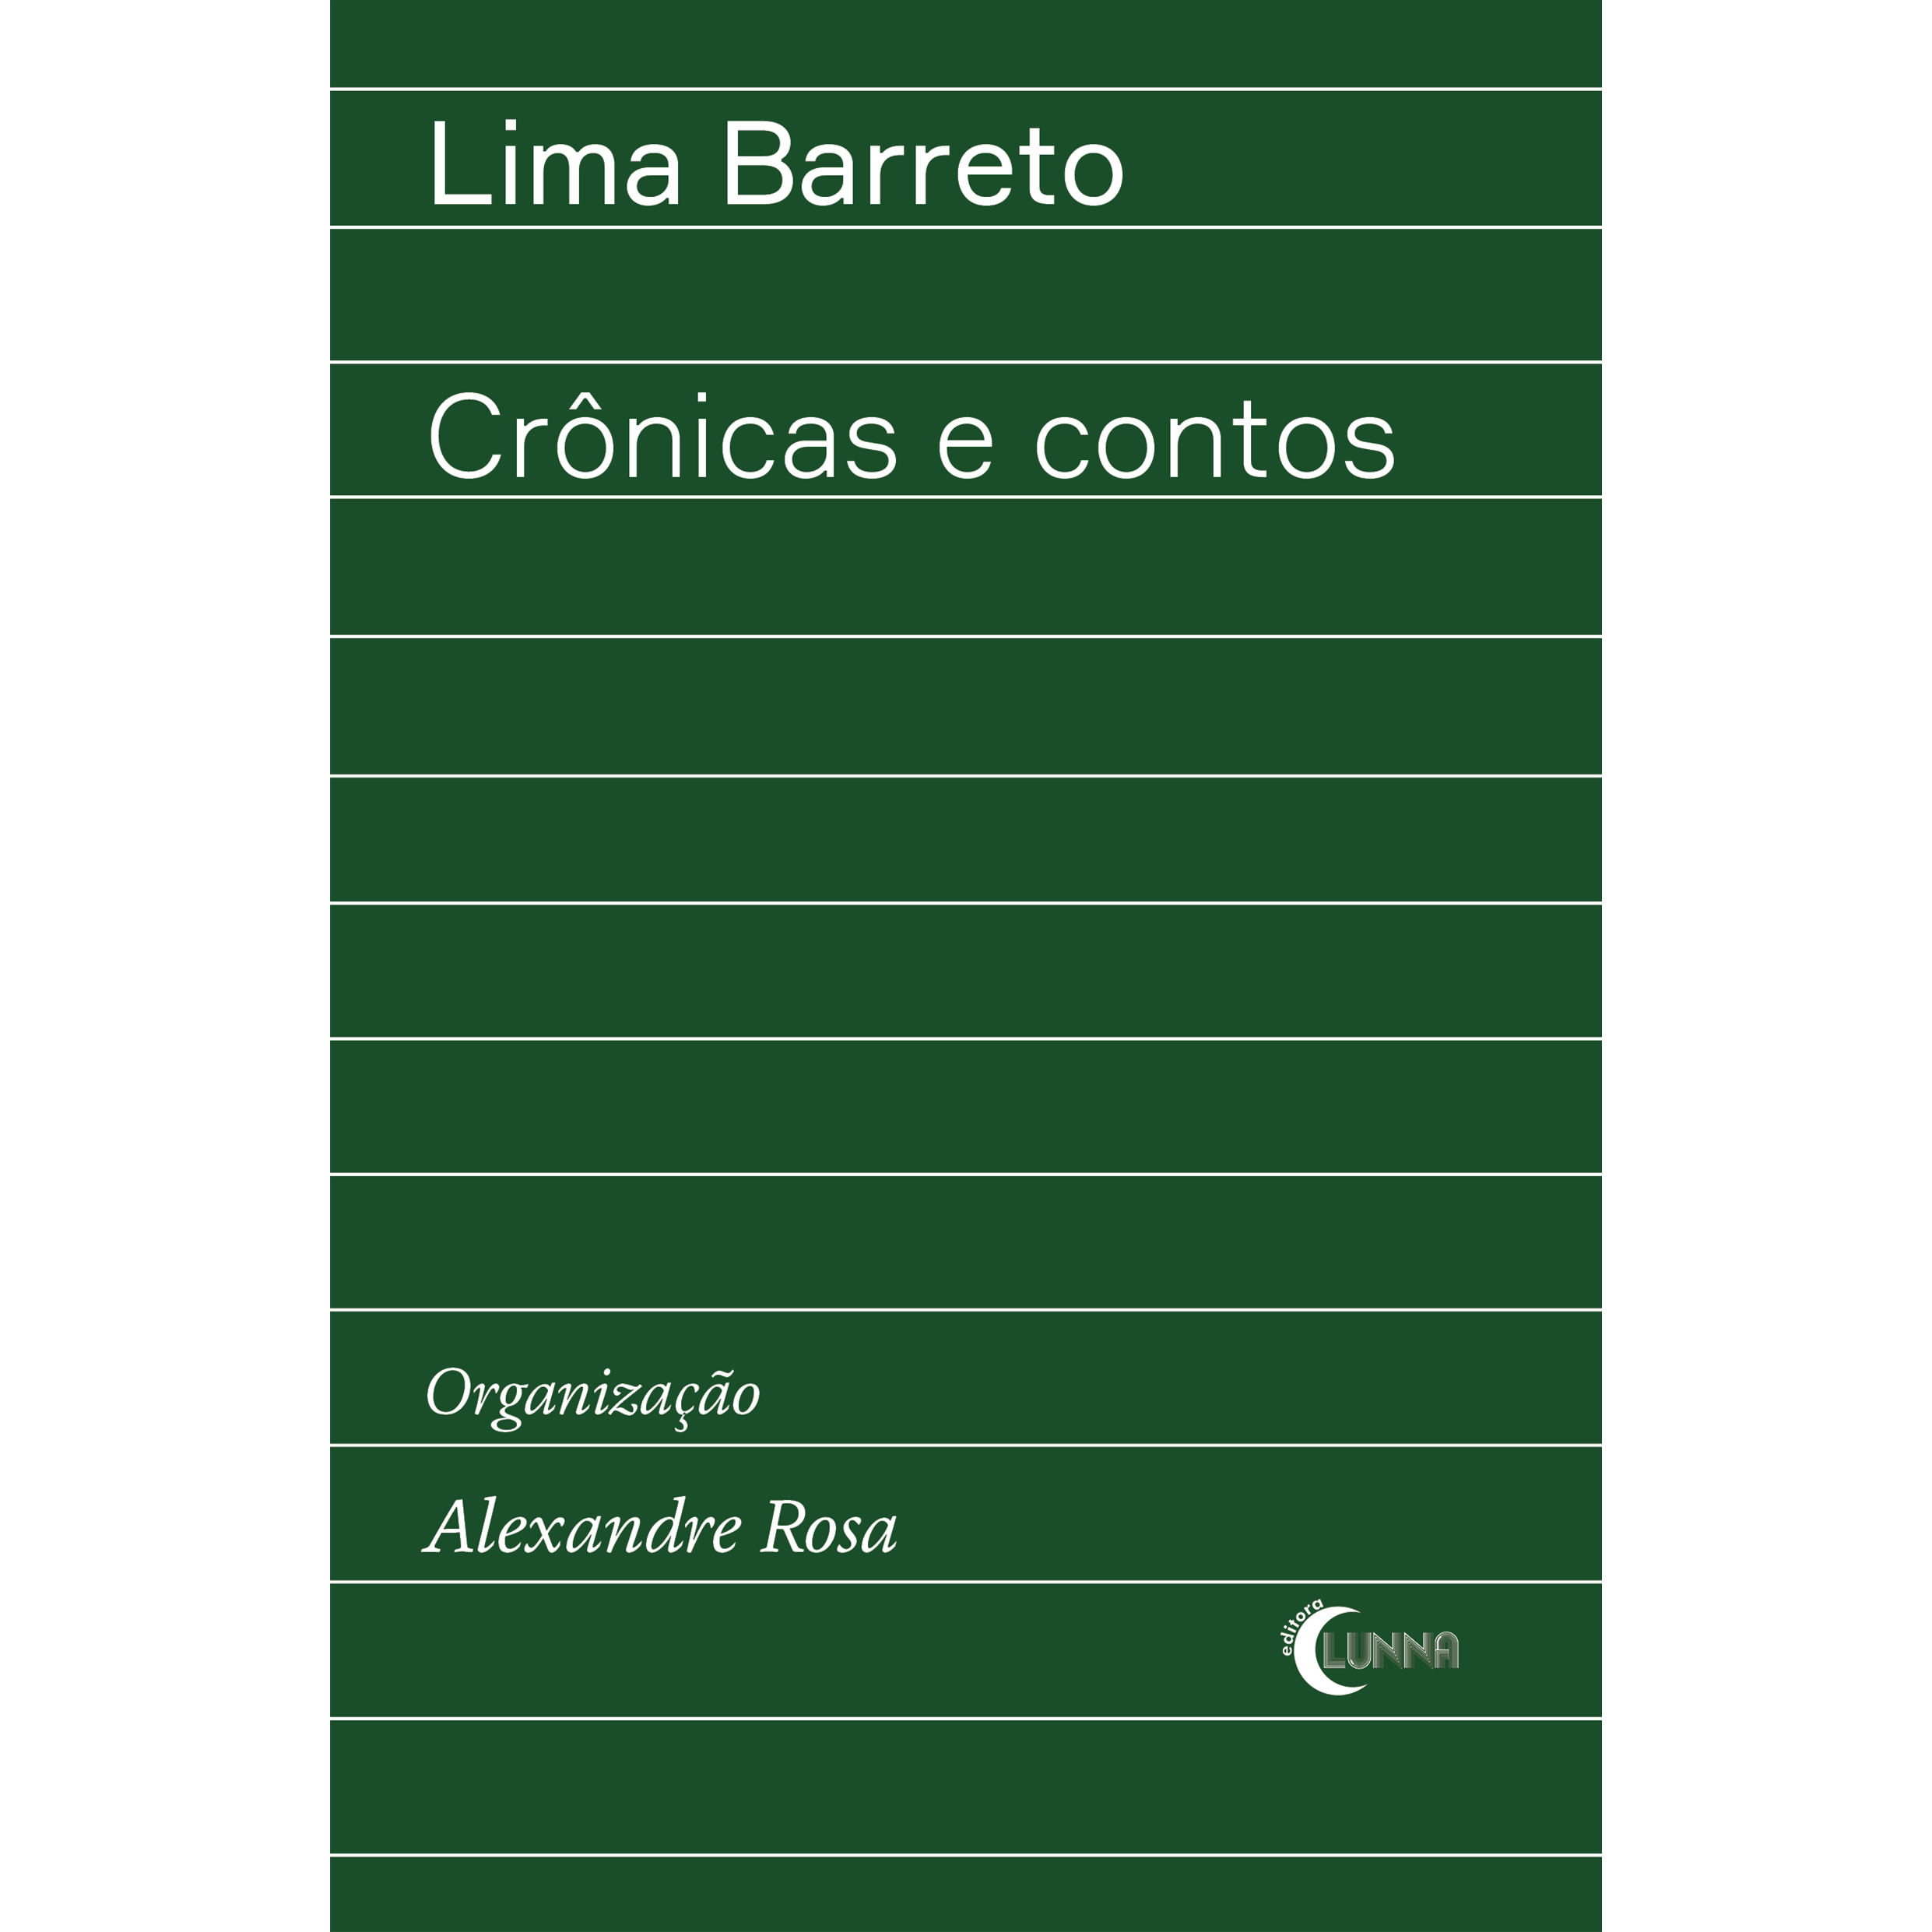
\includegraphics[width=40mm]{./grid/barreto.png}}
\subfloat{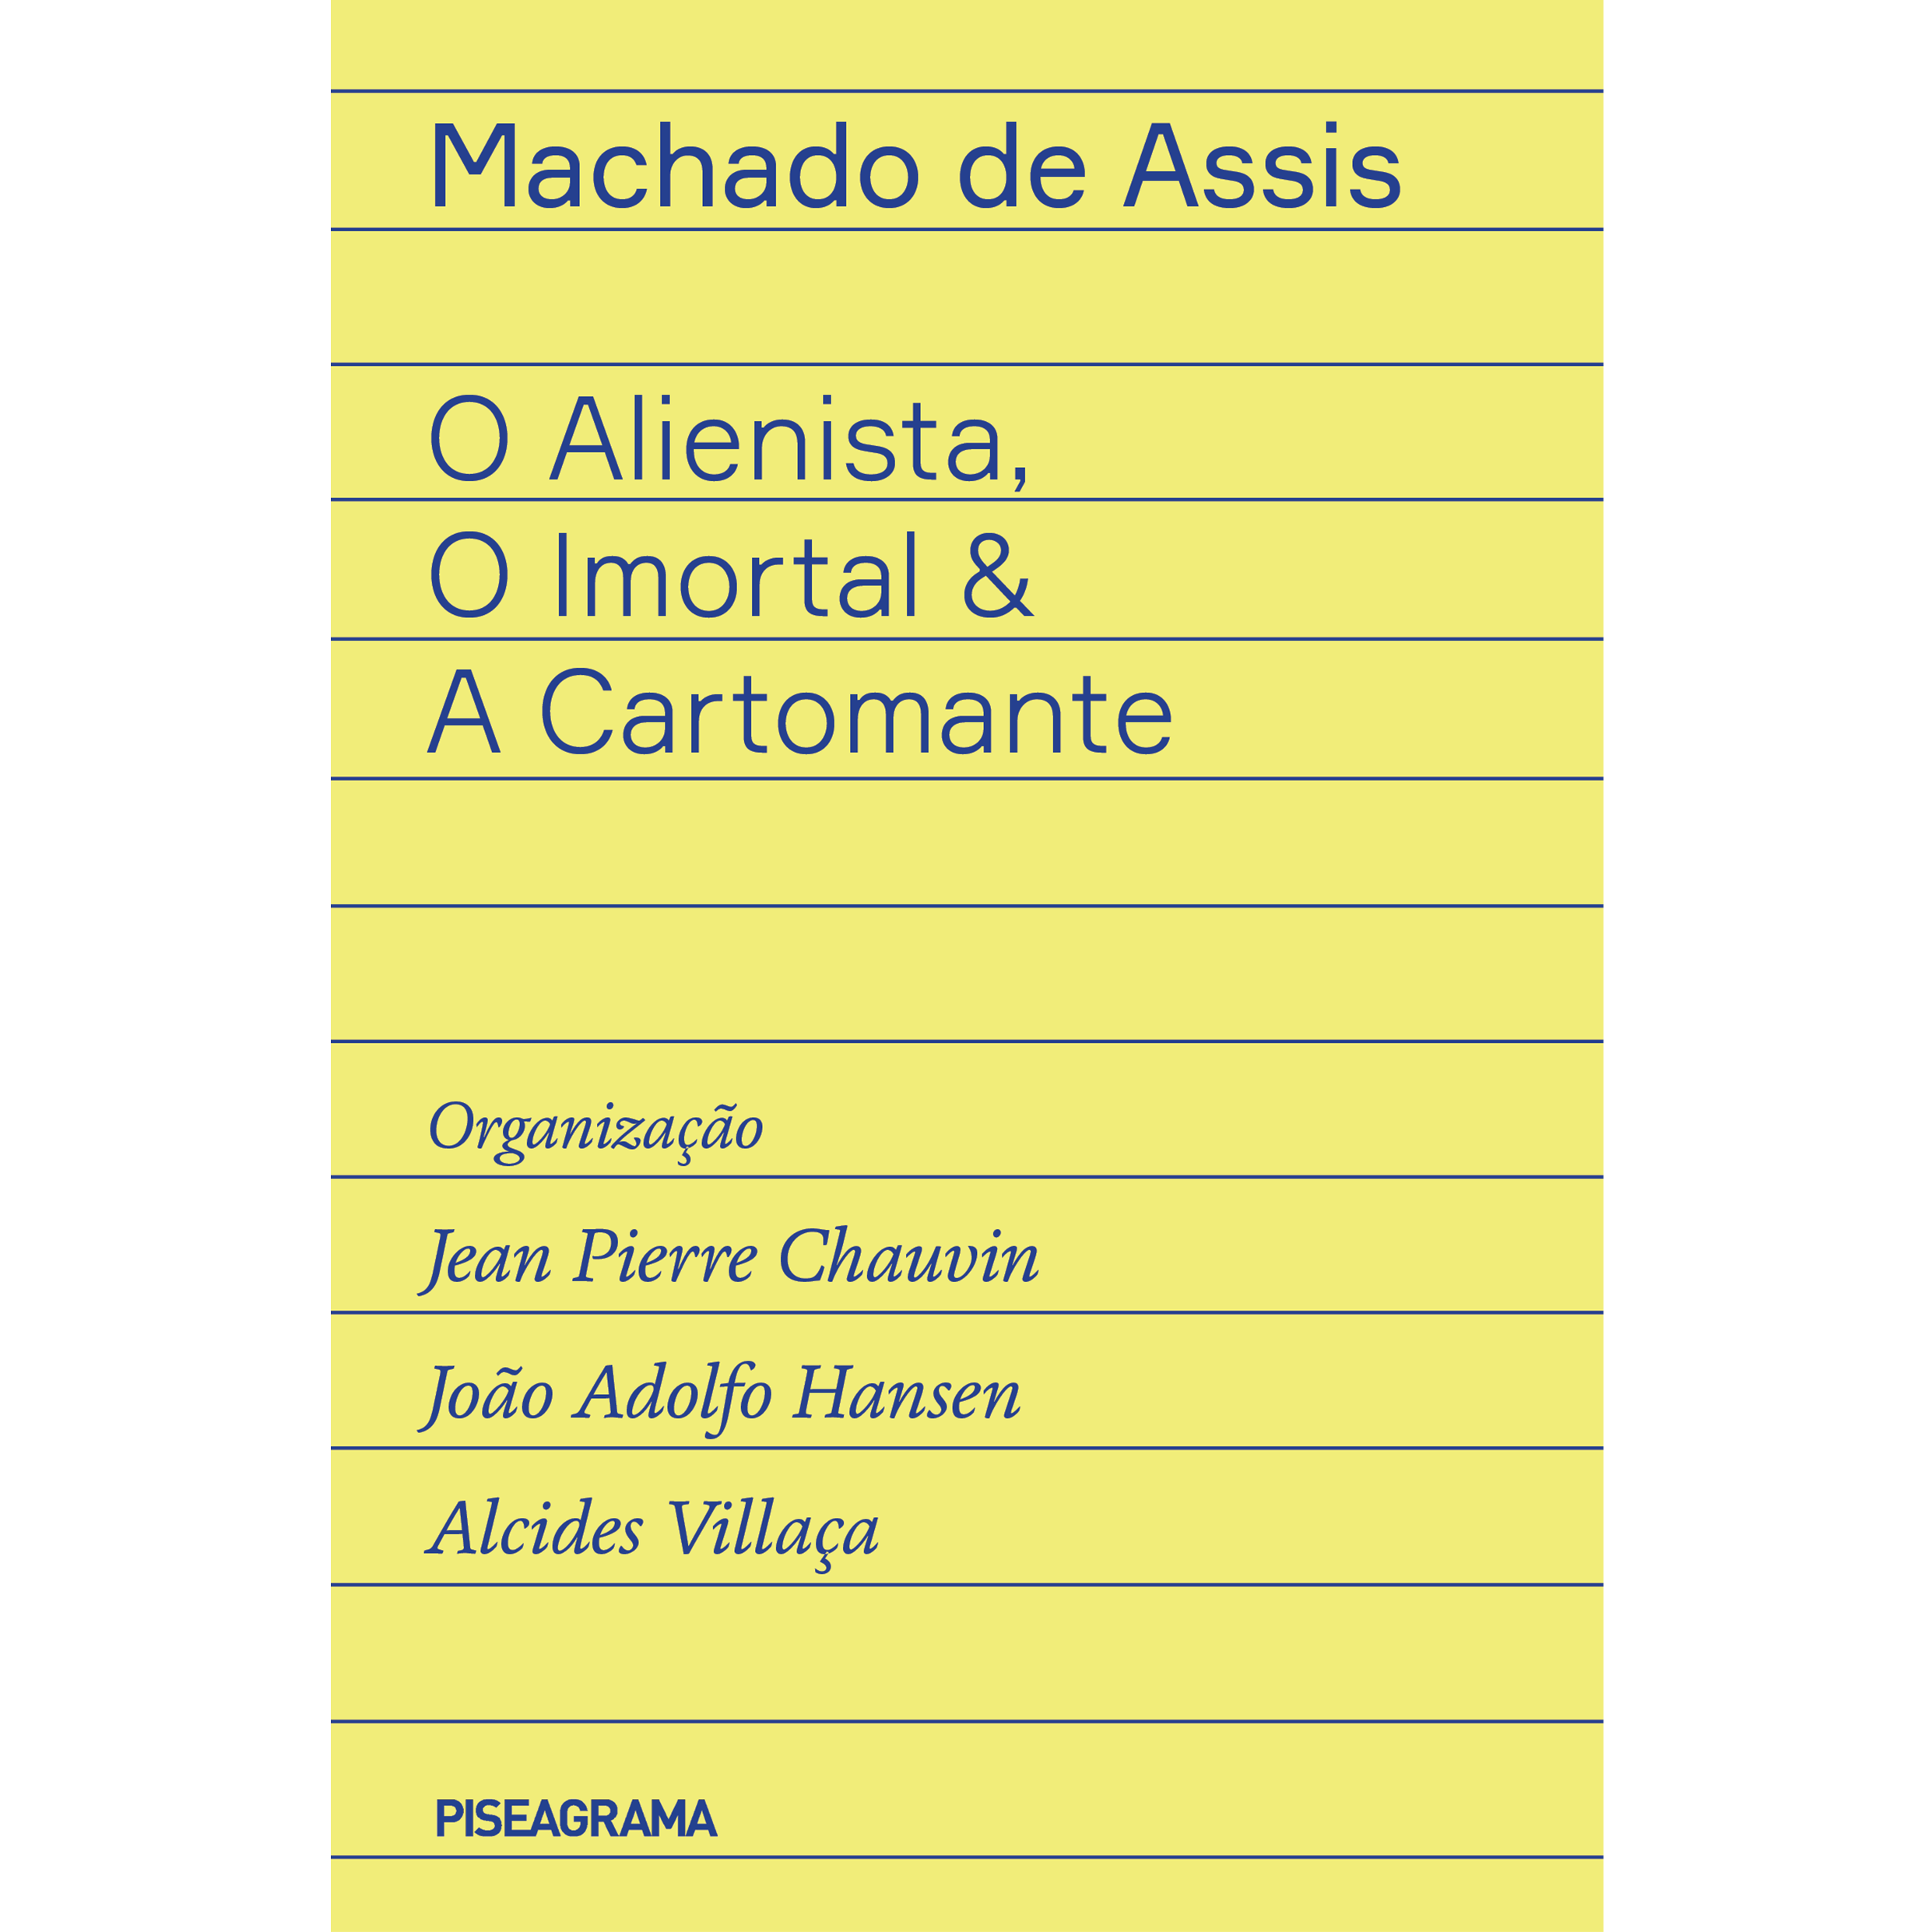
\includegraphics[width=40mm]{./grid/alienista.png}}\\\hspace*{.5cm}
\vspace{.5cm}
\subfloat{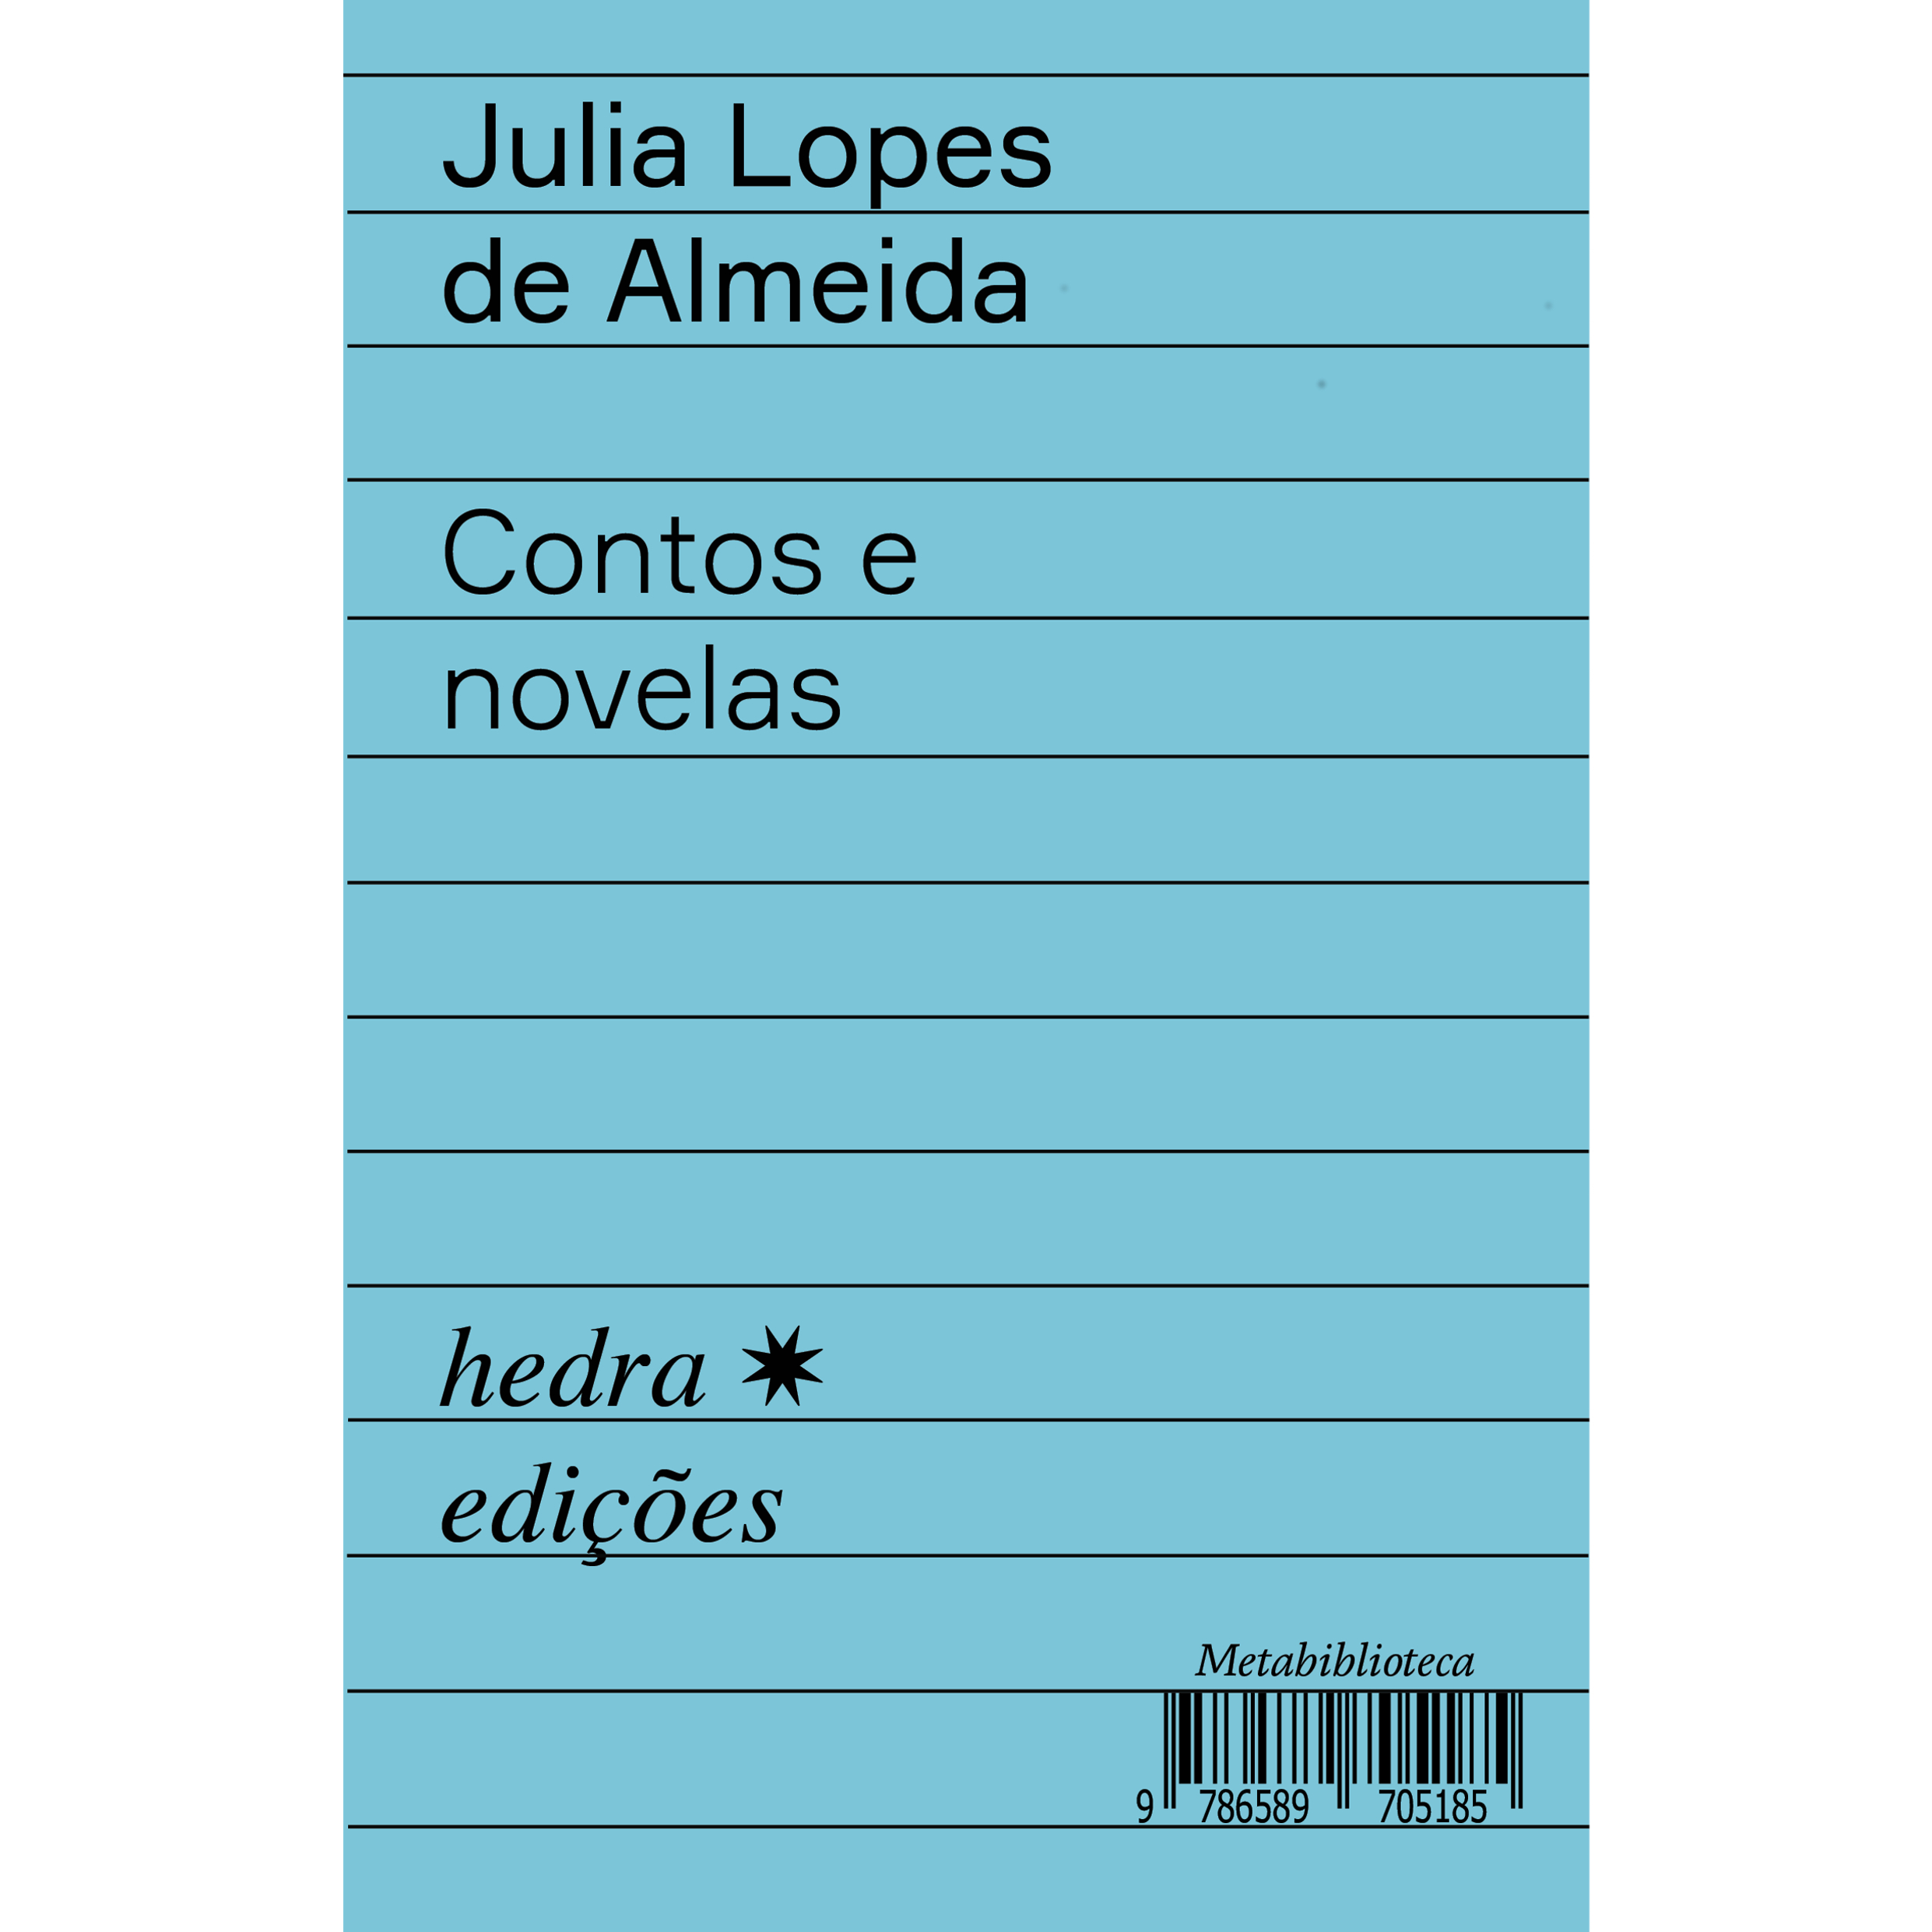
\includegraphics[width=40mm]{./grid/almeida.png}}
\subfloat{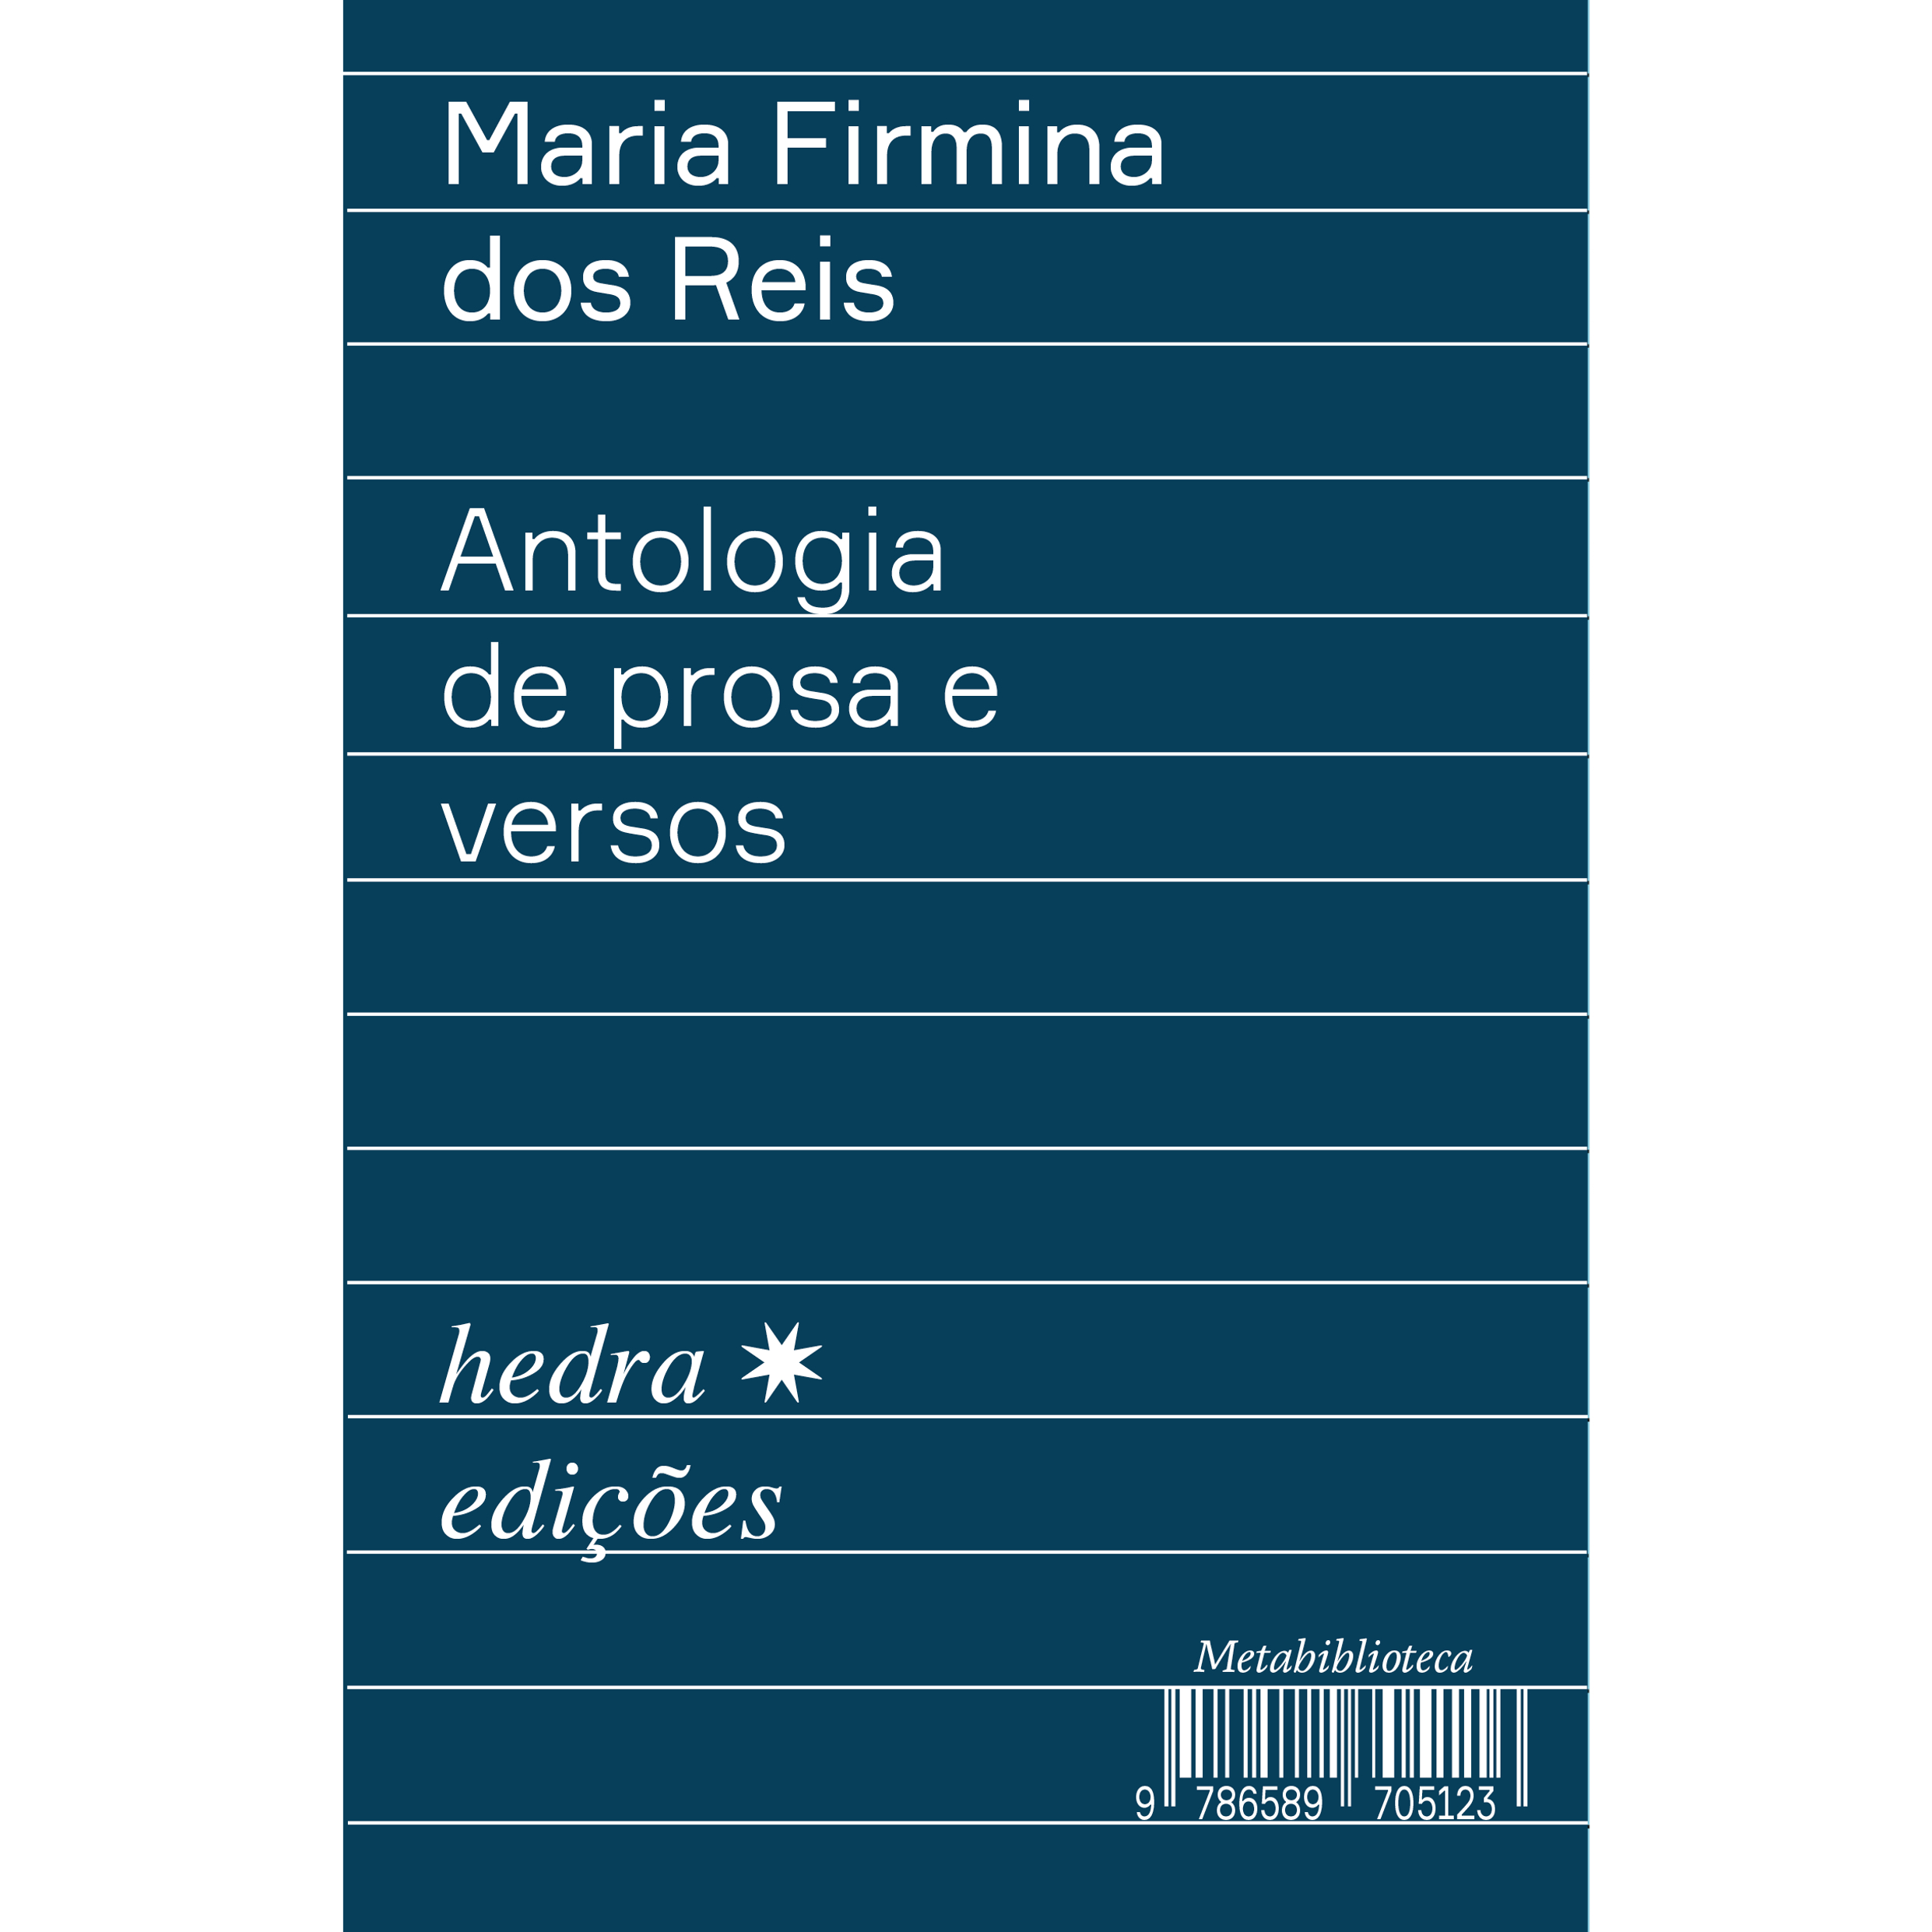
\includegraphics[width=40mm]{./grid/firmina.png}}
\subfloat{
\includegraphics[width=40mm]{./grid/diario.png}}\\\hspace*{.5cm}
\vspace{.5cm}
\subfloat{
\includegraphics[width=40mm]{./grid/brown.png}}
\subfloat{
\includegraphics[width=40mm]{./grid/harriet.png}}
\subfloat{
\includegraphics[width=40mm]{./grid/nascidos.png}}\\\hspace*{.5cm}
\vspace{.5cm}
\subfloat{
\includegraphics[width=40mm]{./grid/robinson.png}}
\subfloat{
\includegraphics[width=40mm]{./grid/ivan.png}}
\subfloat{
\includegraphics[width=40mm]{./grid/stoker.png}}\\
\end{tabular}
\end{figure}

\pagebreak

\pagestyle{grid}

\begin{figure}[!htbp]
\begin{tabular}{cccc}

\vspace{.5cm}
\hspace*{.5cm}
\subfloat{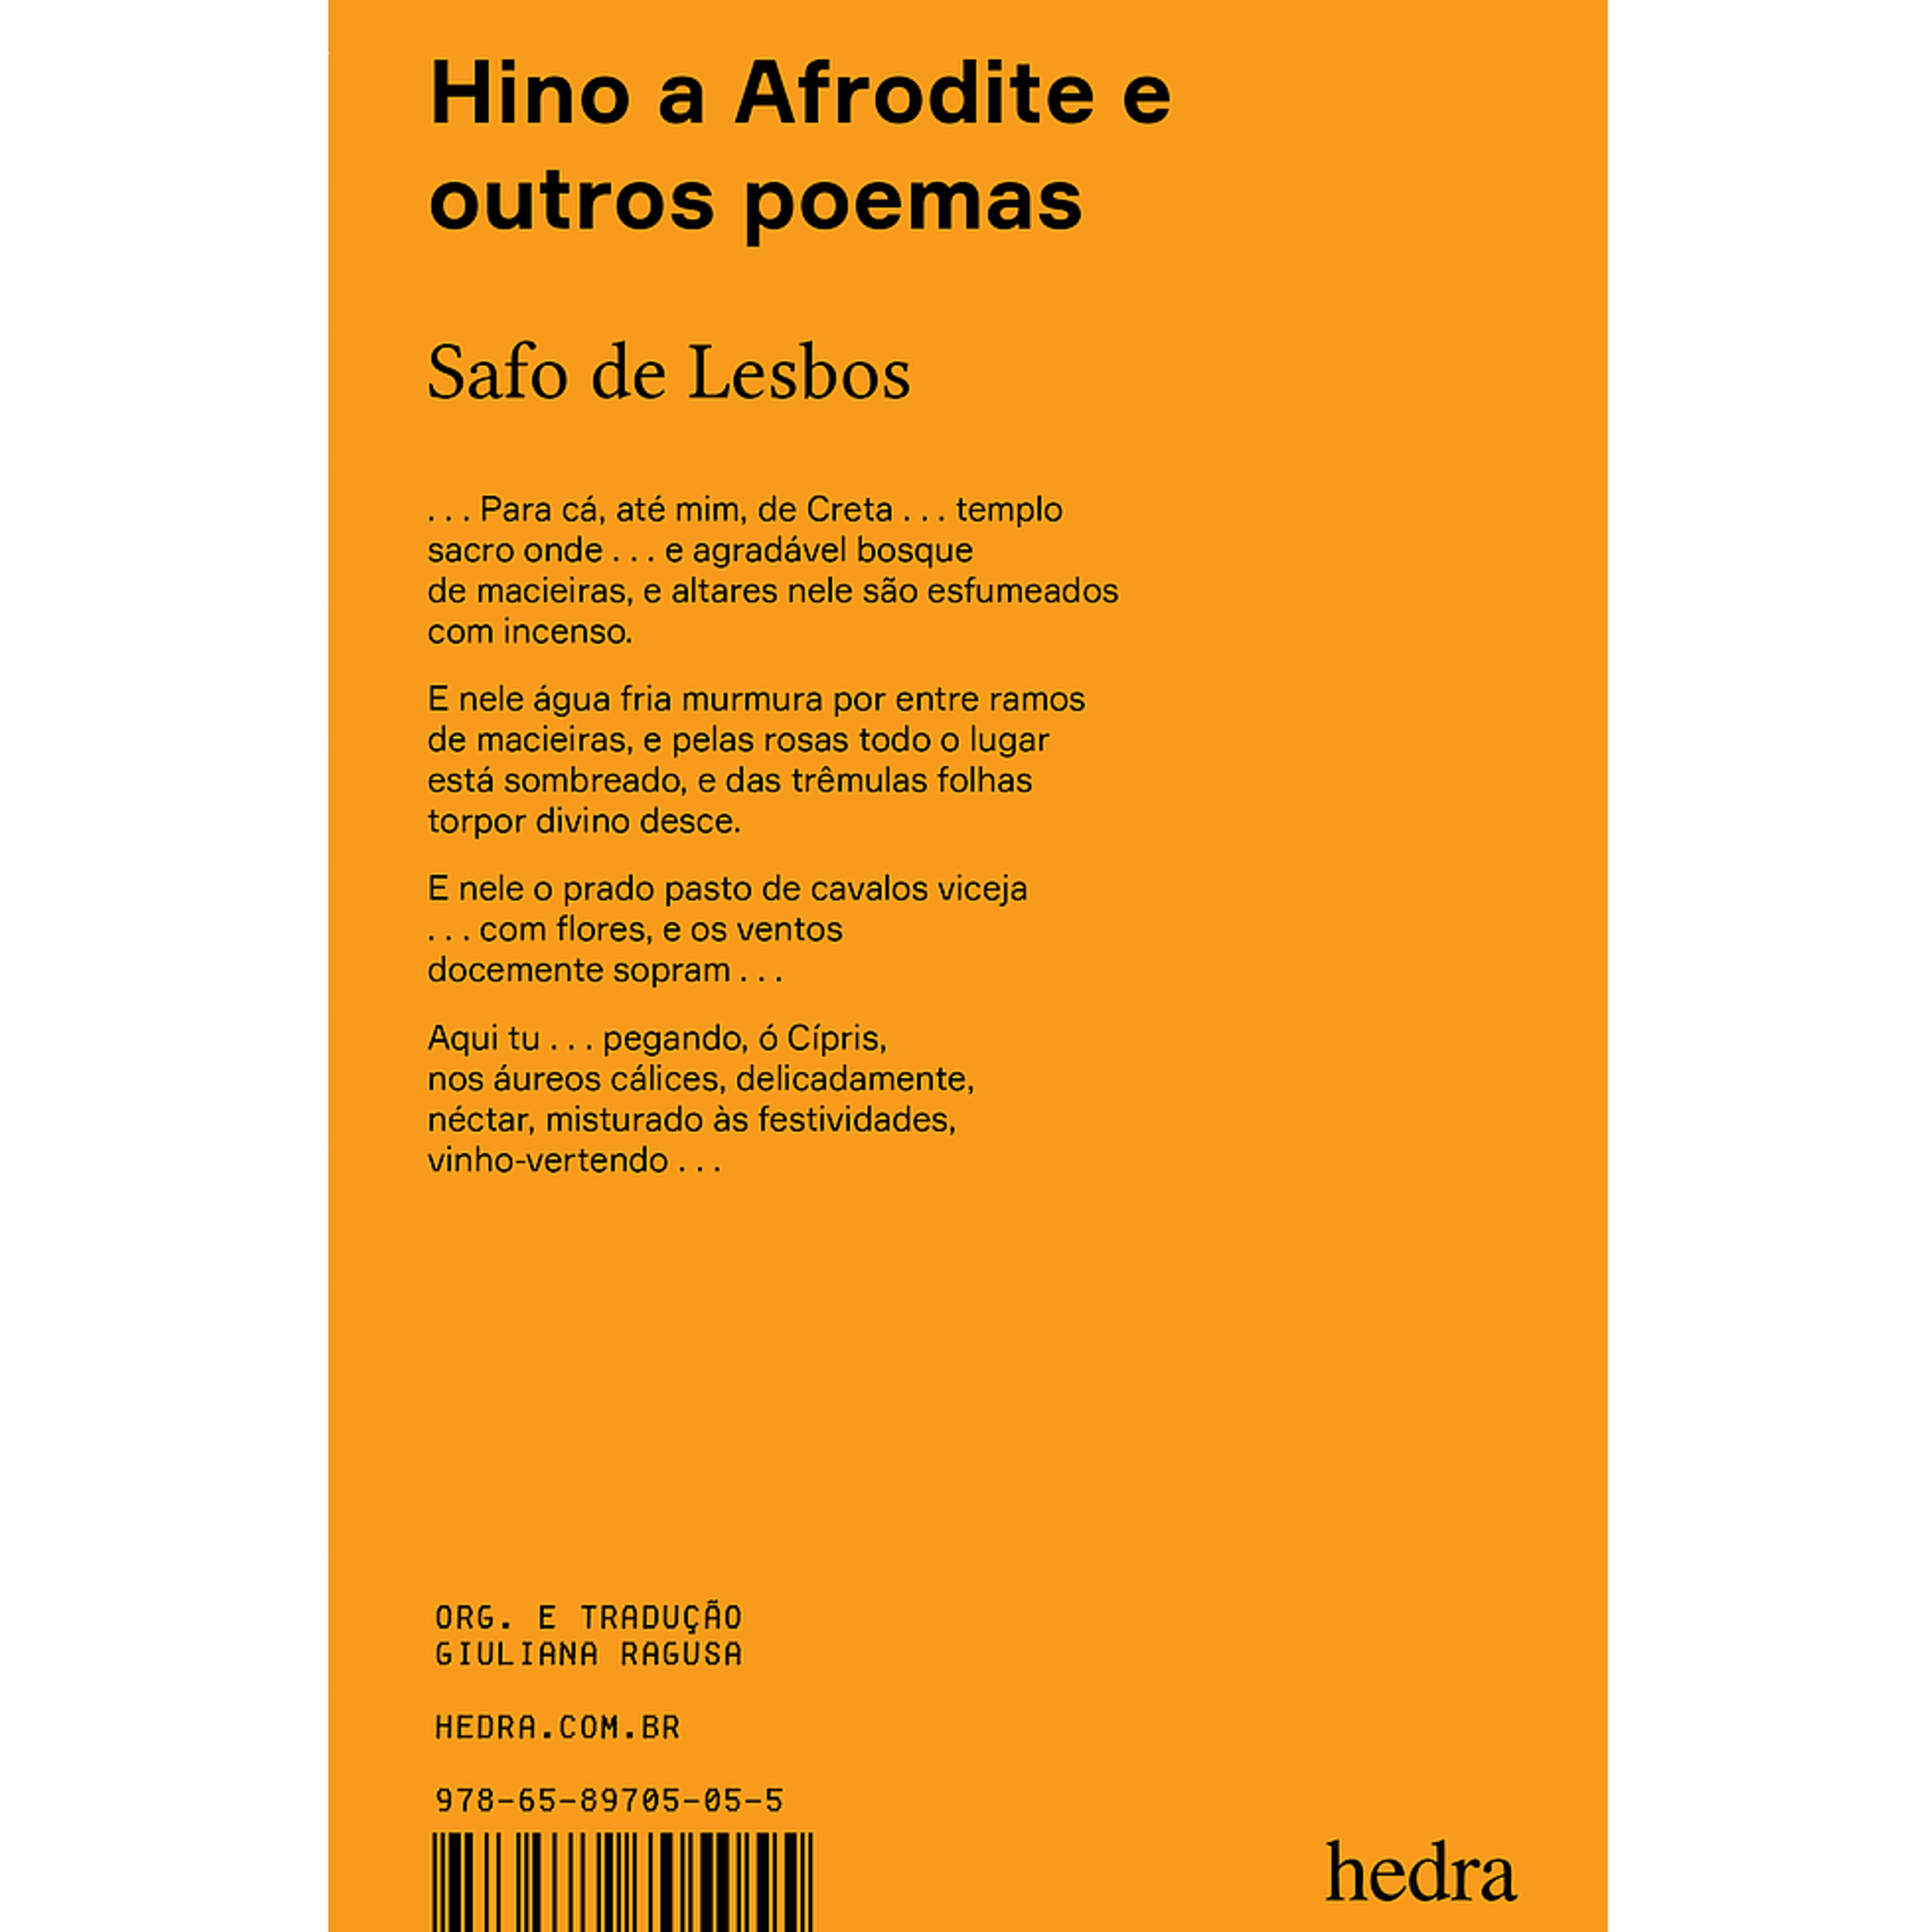
\includegraphics[width=40mm]{./grid/safo.png}}
\subfloat{
\includegraphics[width=40mm]{./grid/medico.png}}
\subfloat{
\includegraphics[width=40mm]{./grid/rashomon.png}}\\\hspace*{.5cm}
\end{tabular}
\end{figure}

\pagebreak

\pagestyle{hedra}
\label{hedra}

%\begin{textblock*}{5.625in}(0pt,0pt)%
%\vspace*{-3.5cm}
%\hspace*{-2.77cm}\includegraphics*[width=175.2mm]{./propagandas/HEDRA.pdf}
%\end{textblock*}

%\pagebreak

\begin{center}
\hspace*{-3.6cm}\raisebox{5cm}{\rotatebox[origin=t]{90}{\huge\textbf{Seleção especial}}}
\hspace*{3.1cm}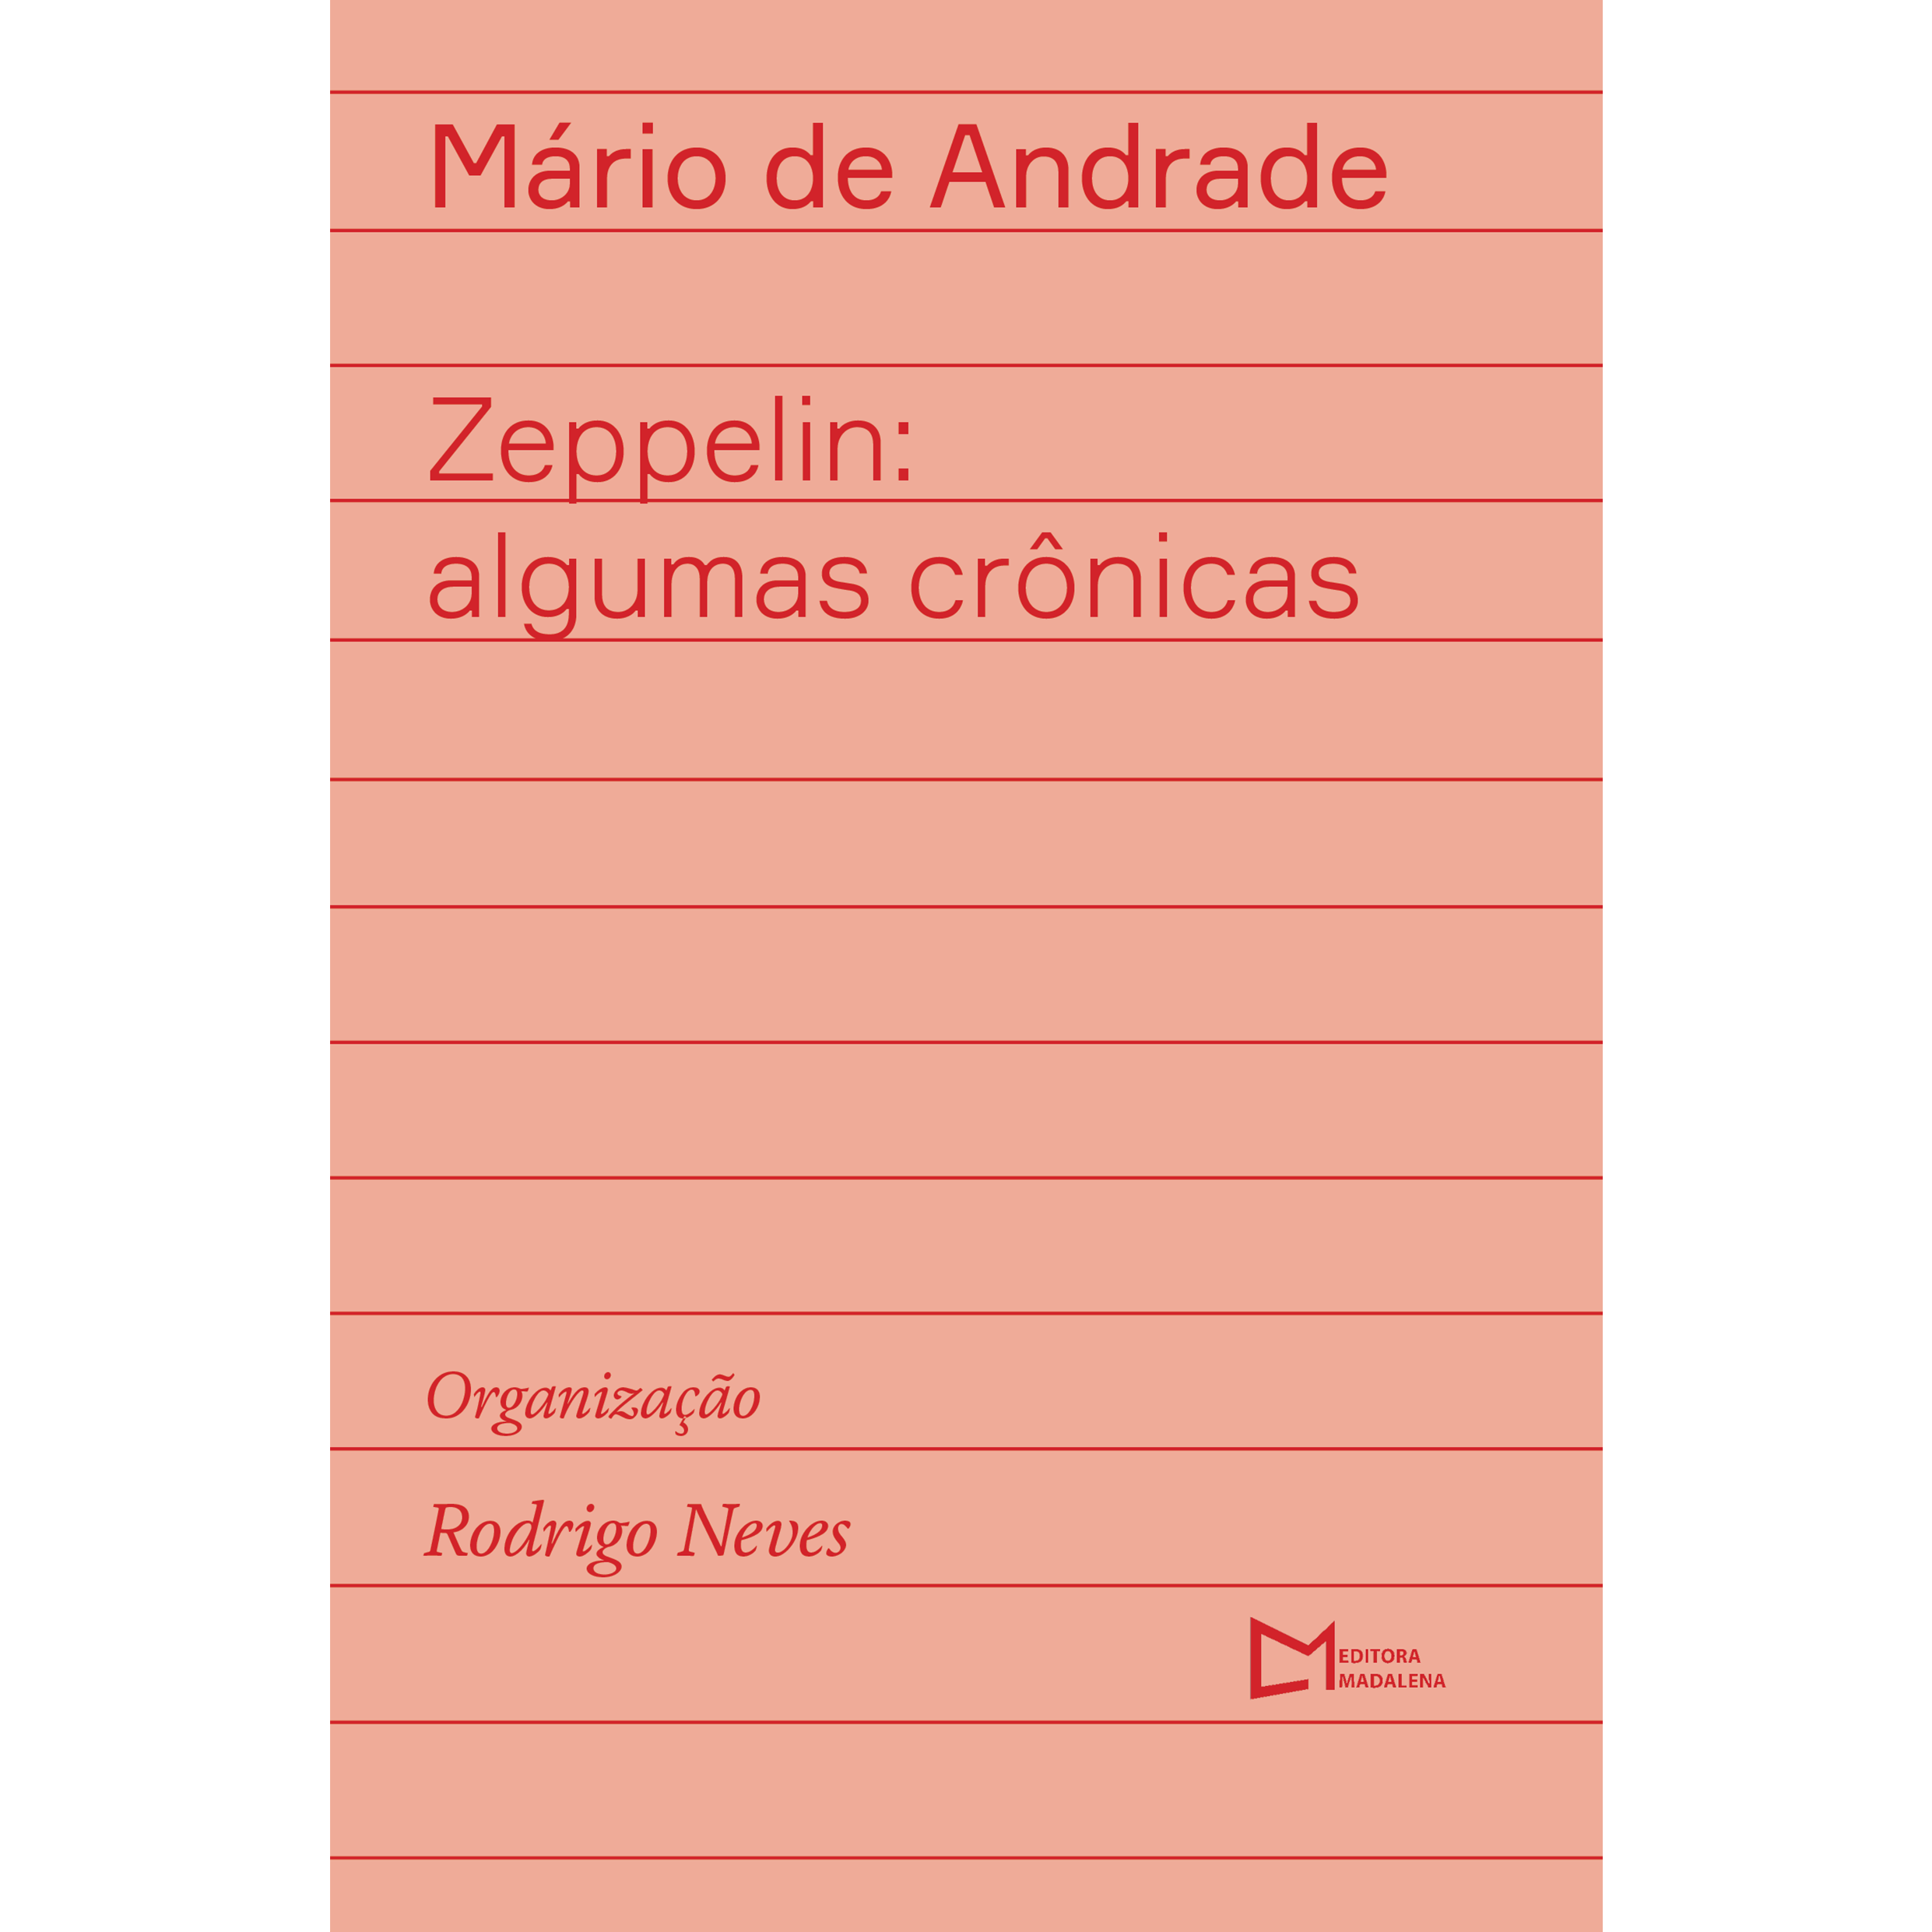
\includegraphics[width=74mm]{./grid/zepelin.png}
\end{center}

\hspace*{-7cm}\hrulefill\hspace*{-7cm}

\medskip

\noindent{}\textit{Zeppelin e outros contos} reúne crônicas extraídas dos livros \textit{Os
filhos da Candinha} (1943), \textit{Será o Benedito!} (1992) e \textit{Táxi e crônicas no Diário Nacional} (1976). Mário de Andrade é famoso por ser um escritor de gêneros diversos e a crônica é o gênero mais praticado em sua obra.
Com textos publicados originalmente em jornais e revistas como o \textit{Diário Nacional} e o \textit{Suplemento em Rotogravura} do Estado de São Paulo, os contos trazem temas importantes, como os limites entre realidade e ficção, dramas familiares, a valorização da cultura popular, os contrastes sociais acentuados pelo desenvolvimento acelerado do país e a diversidade na formação da nossa identidade.

\vfill

\noindent\begin{minipage}[c]{1\linewidth}
{\small\textbf{
\hspace*{-.1cm}Editora: Hedra\\
Título: Zeppelin e outros contos\\
Autor: Mário de Andrade\\ 
%ISBN: 978-65-89705-20-8\\
Páginas: 240\\
Formato: 13,3x21cm\\
Preço: R\$ 88,00\\
}}
\end{minipage}

\pagebreak

\begin{center}
\hspace*{-3.6cm}
\hspace*{3.1cm}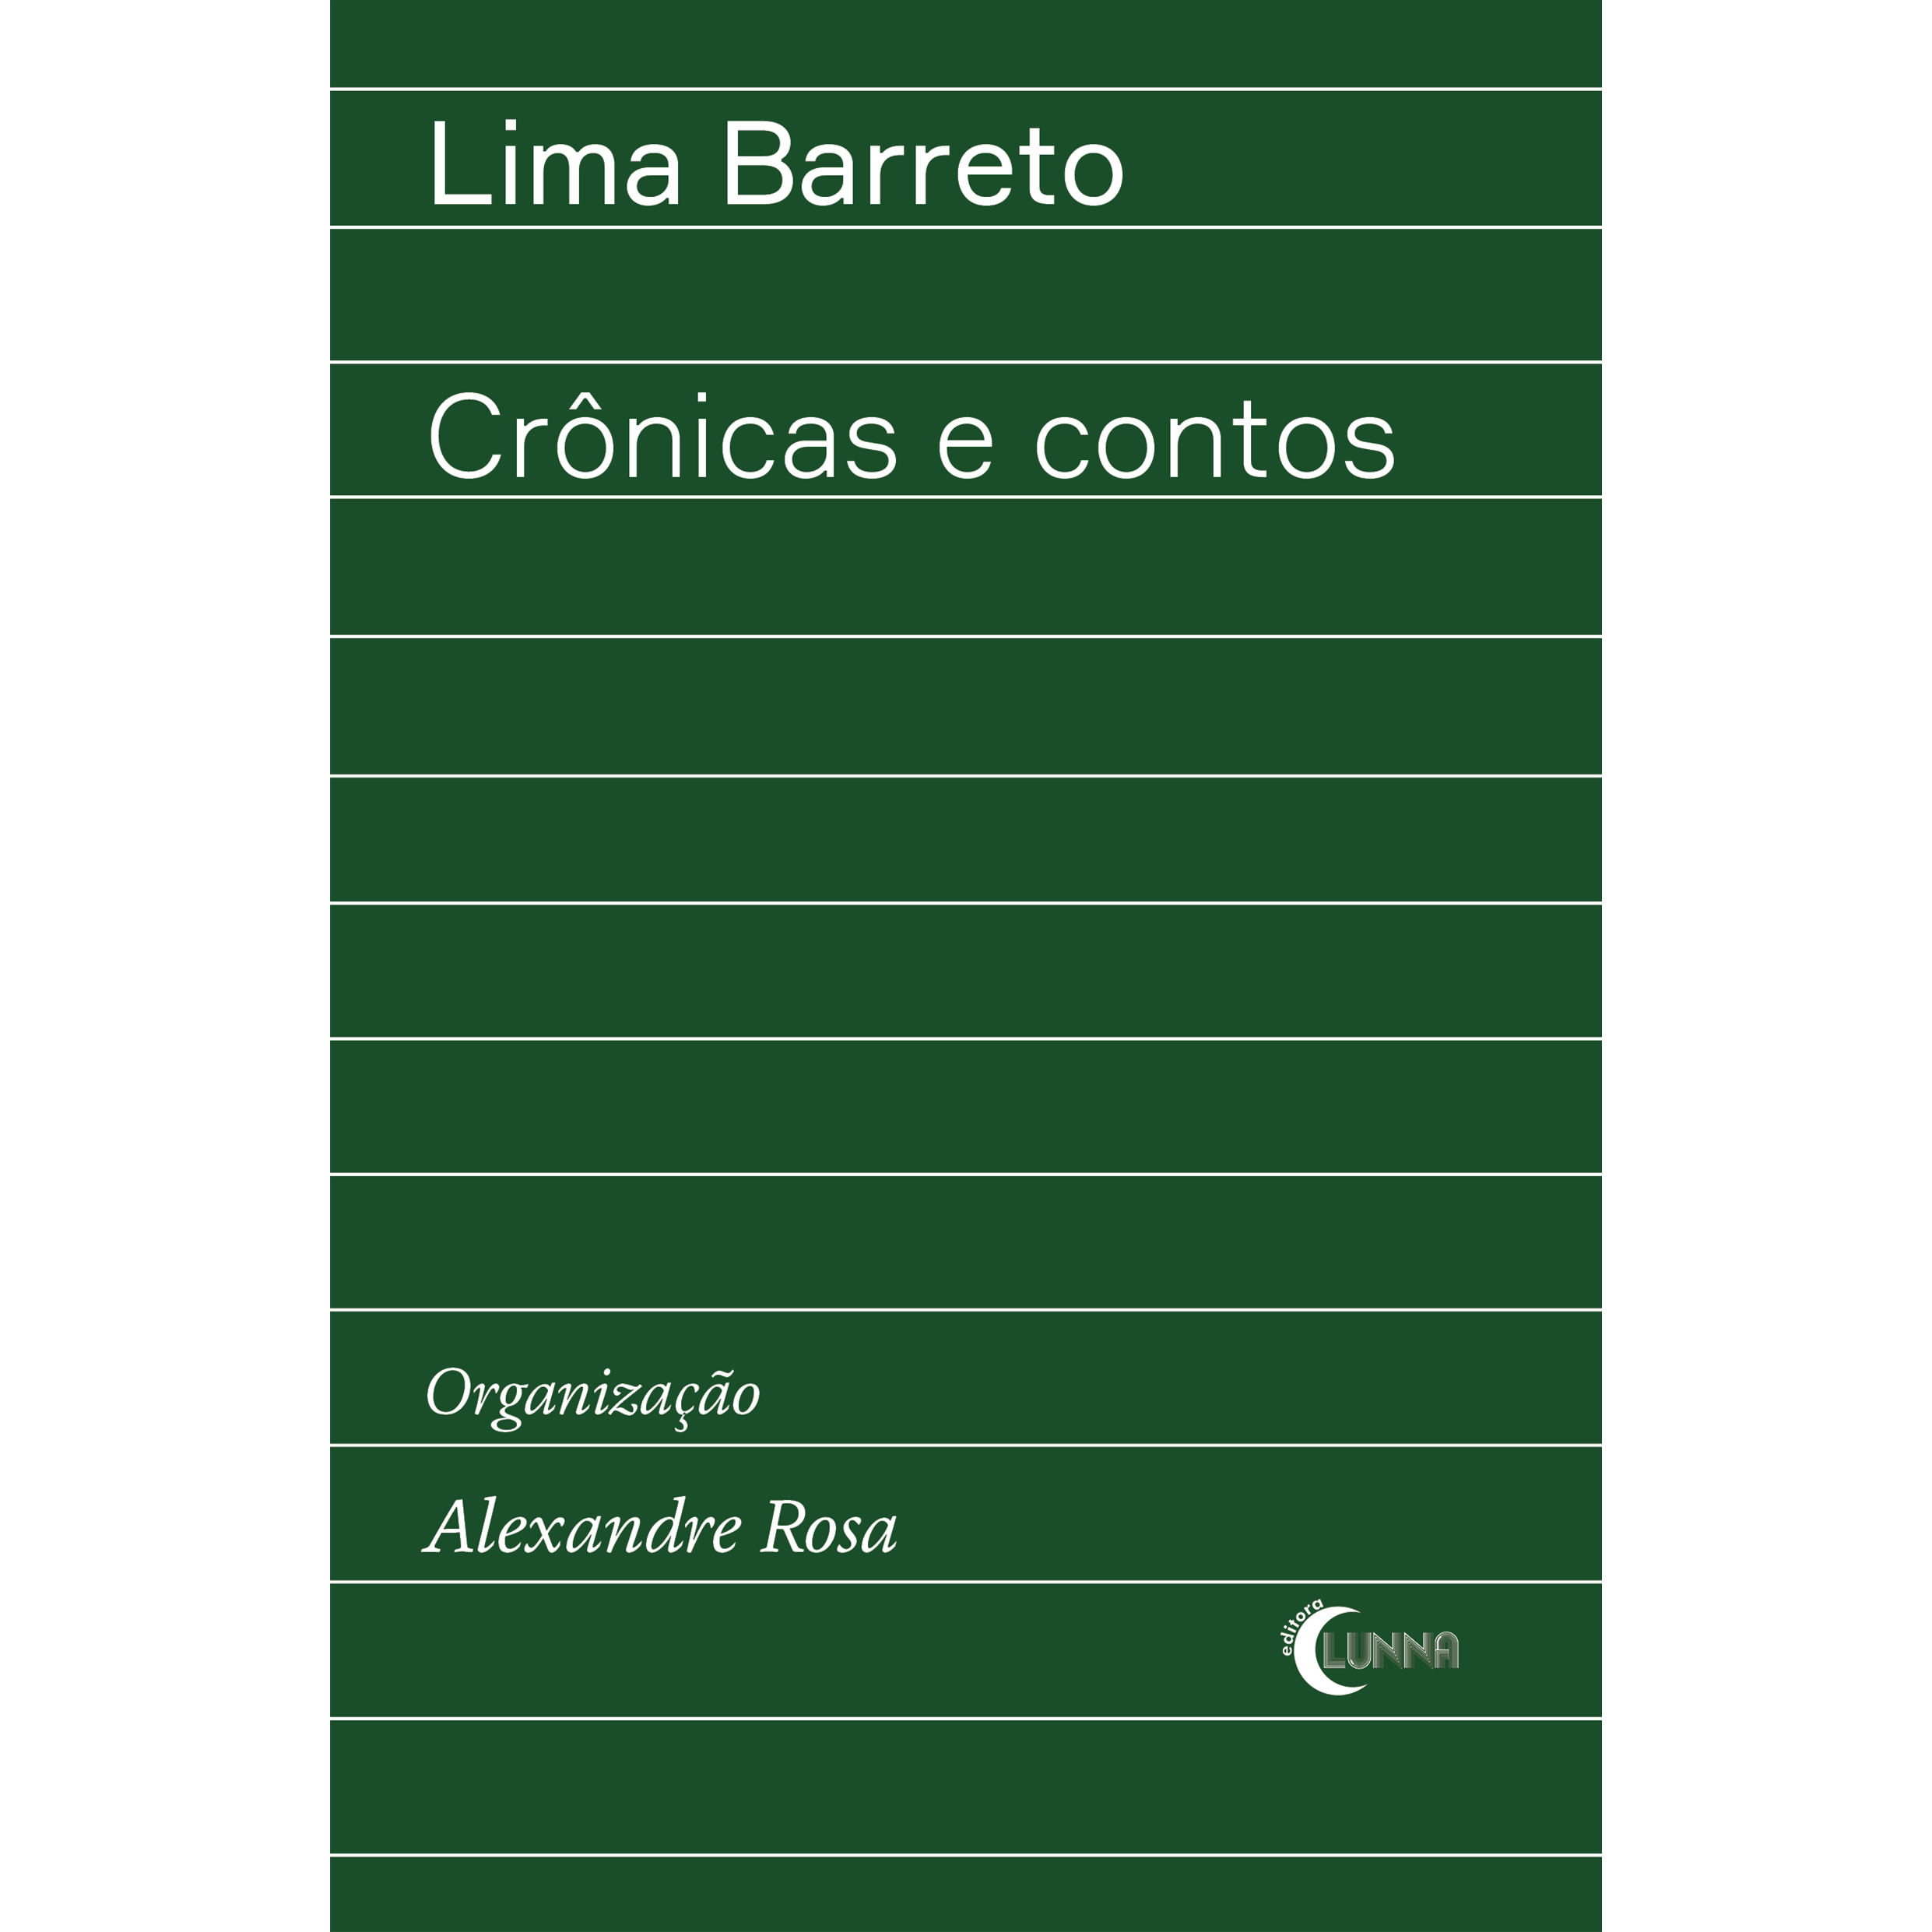
\includegraphics[width=74mm]{./grid/barreto.png}
\end{center}

\hspace*{-7cm}\hrulefill\hspace*{-7cm}

\medskip

\noindent{}A presente antologia reúne crônicas e contos de Lima Barreto. A grande maioria desses textos foi publicada em jornais e revistas da época, posteriormente agrupados em livros e coletâneas. A primeira parte, dedicada às crônicas, foi pensada de modo a reunir os textos em pequenos conjuntos temáticos. Alguns assuntos que organizam a primeira parte são: \textit{autobiografia}; \textit{cotidiano e vida nos subúrbios}; \textit{futebol}; \textit{nossa política e nossos políticos}; \textit{violência contra as mulheres} e \textit{humor}. A segunda parte reúne o que de mais significativo Lima Barreto escreveu sob o gênero do conto: ``O homem que sabia javanês'', ``A nova Califórnia'' e ``Como o `homem' chegou'' podem ser considerados como grandes realizações da literatura brasileira.
\vfill

\noindent\begin{minipage}[c]{1\linewidth}
{\small\textbf{
\hspace*{-.1cm}Editora: Hedra\\
Título: Crônicas e contos\\
Autor: Lima Barreto\\ 
%ISBN: 978-65-89705-05-5\\
Páginas: 344\\
Formato: 13,3x21cm\\
Preço: R\$ 120,00\\
}}
\end{minipage}

\pagebreak

\begin{center}
\hspace*{-3.6cm}\raisebox{5cm}{\rotatebox[origin=t]{90}{\huge\textbf{Seleção especial}}}
\hspace*{3.1cm}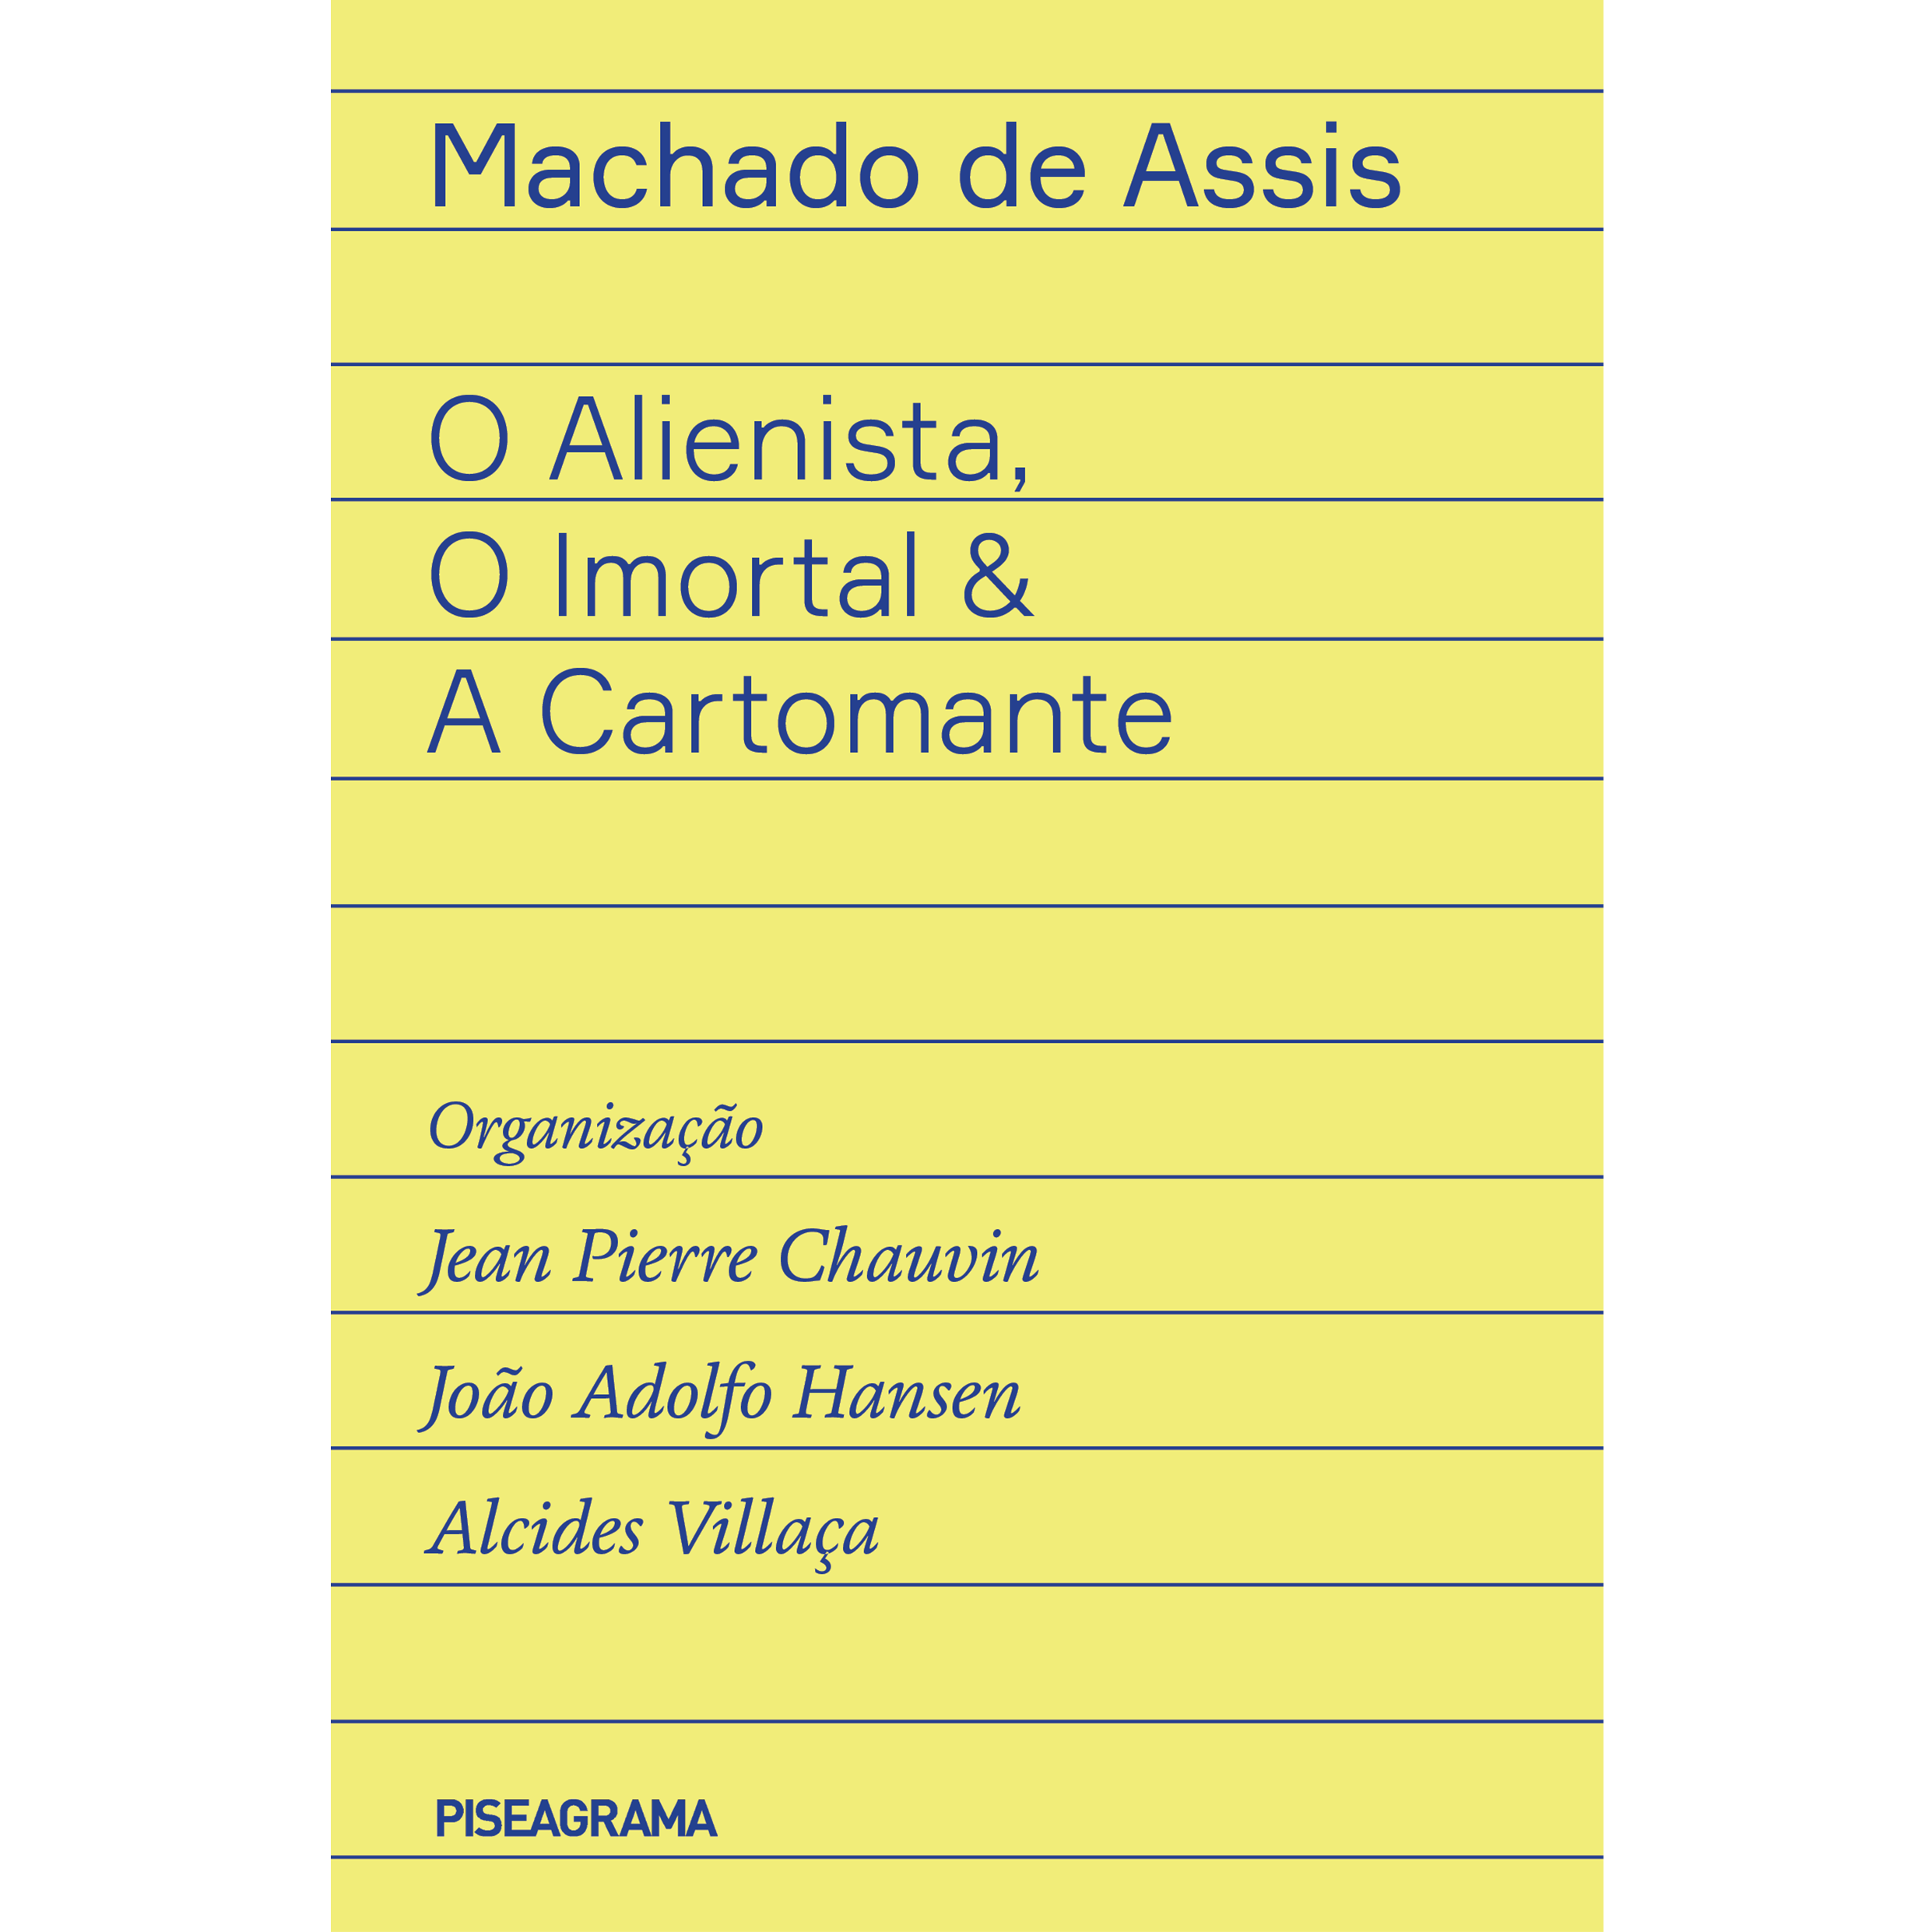
\includegraphics[width=74mm]{./grid/alienista.png}
\end{center}

\hspace*{-7cm}\hrulefill\hspace*{-7cm}

\medskip

\noindent{}As três narrativas de Machado de Assis aqui organizadas foram, originalmente,
publicadas em revista. ``O alienista'' saiu na Revista \textit{A estação} --- periódico voltado para o público feminino que circulou no Rio de Janeiro entre 1879 e 1904 --- entre 15 de outubro de 1881 e 15 de março de 1882. Foi posteriormente coletado em \textit{Papéis avulsos}. Nessa mesma revista saiu ``O imortal'' em 1882. Dois anos depois, em 28 de novembro de 1884, ``A cartomante'' foi publica na revistsa \textit{Gazeta de notícias}, e depois coletada no livro de contos \textit{Várias histórias}. Textos de difícil classificação, entre o conto e a novela, são algumas das obras mais conhecidas de Machado de Assis. São especialmente impressionantes, principalmente por se aproximarem do gênero fantástico.

\vfill

\noindent\begin{minipage}[c]{1\linewidth}
{\small\textbf{
\hspace*{-.1cm}Editora: Hedra\\
Título: O Alienista, O Imortal e A Cartomante\\
Autor: Machado de Assis\\ 
%ISBN: 978-65-89705-12-3\\
Páginas: 210\\
Formato: 13,3x21cm\\
Preço: R\$ 79,40\\
}}
\end{minipage}

\pagebreak

\begin{center}
\hspace*{.5cm}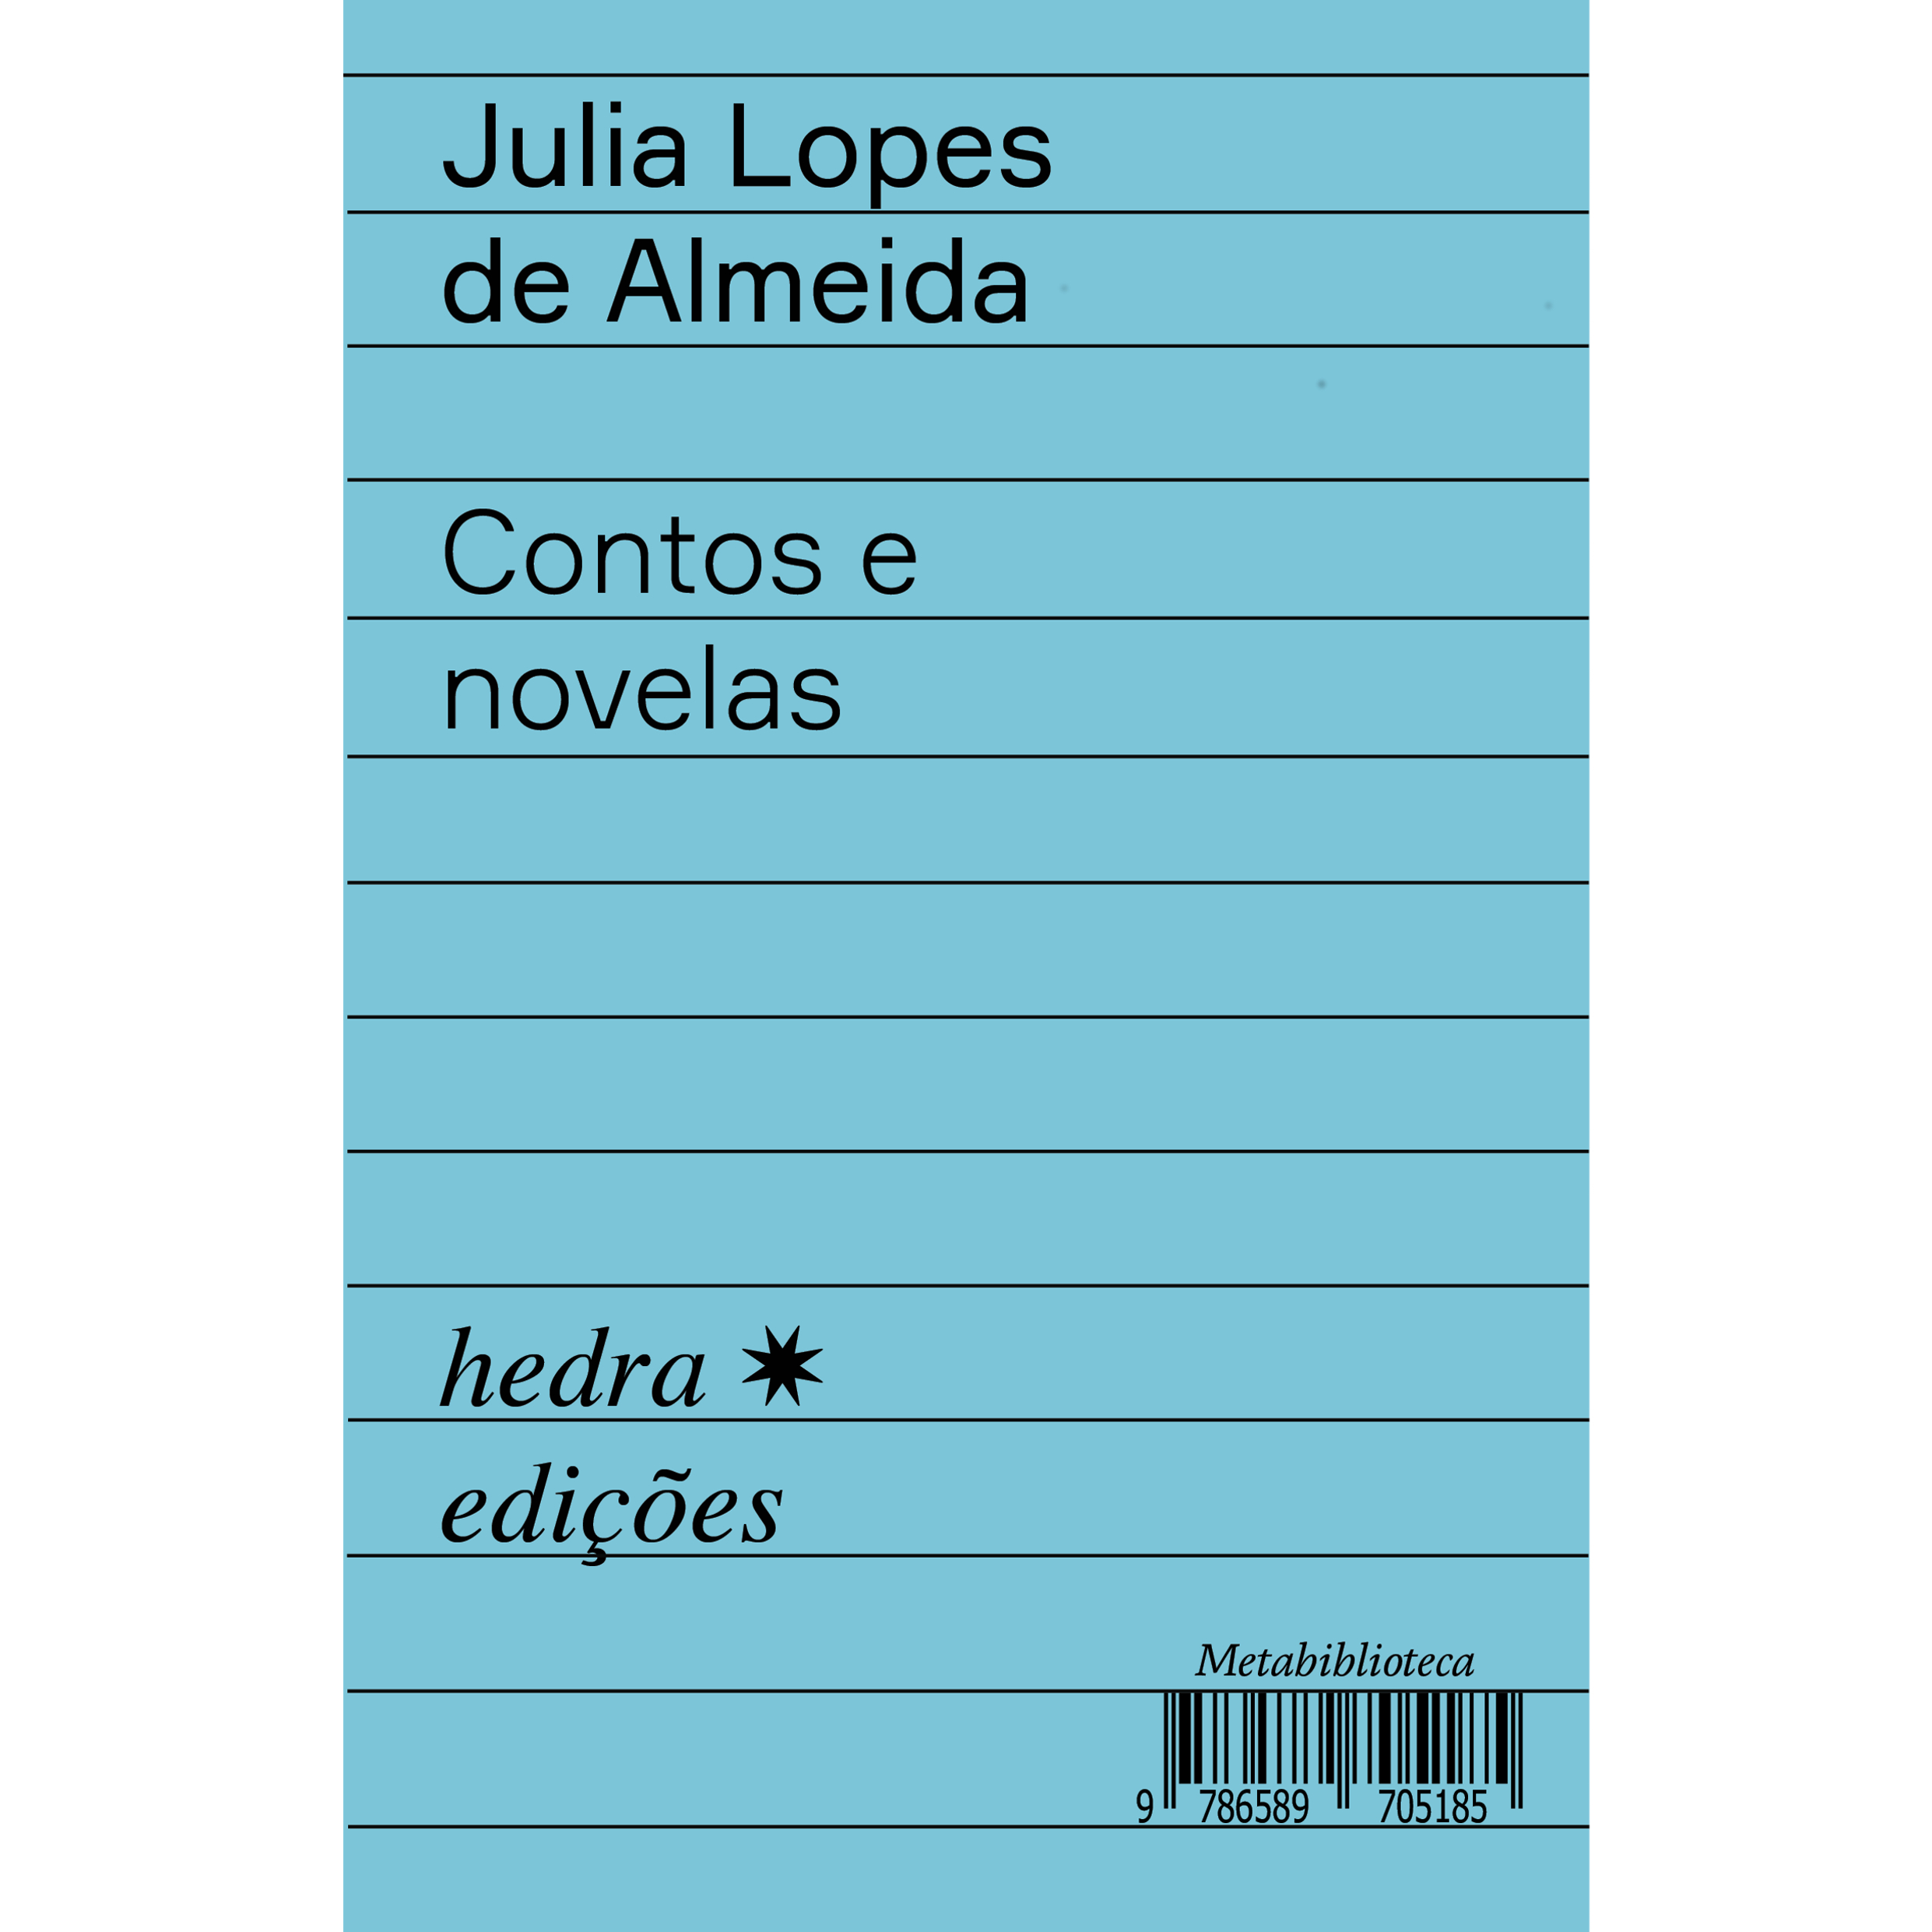
\includegraphics[width=74mm]{./grid/almeida.png}
\end{center}

\hspace*{-7cm}\hrulefill\hspace*{-7cm}

\medskip

\noindent{}\textit{Contos e novelas} é uma antologia de narrativas curtas de Júlia Lopes de Almeida, extraídas de duas de suas obras, \textit{Ânsia eterna} (1903) e \textit{A isca} (1922), em que a escritora apresenta alguns dos principais elementos que caracterizam sua literatura, como a presença do insólito, o lugar da mulher na sociedade patriarcal, os conflitos familiares, as marcas da escravidão e os contrastes sociais, políticos e econômicos, resultantes da modernização. Júlia Lopes de Almeida é uma das escritoras brasileiras mais importantes da virada do século XIX para o XX, mas pouco lida se comparada aos escritores, em face da invisibilidade sofrida pelas escritoras. Esteve também entre os idealizadores da Academia Brasileira de Letras, mas foi preterida a assumir uma das cadeiras entre os fundadores por ser mulher.
\vfill

\noindent\begin{minipage}[c]{.5\linewidth}
{\small\textbf{
\hspace*{-.1cm}Editora: Hedra\\
Título: Contos e novelas\\
Autor: Júlia Lopes de Almeida\\ 
%ISBN: 978-65-89705-16-1\\
Páginas: 216\\
Formato: 13,3x21cm\\
Preço: R\$ 81,30\\
}}
\end{minipage}

\pagebreak

\begin{center}
\hspace*{-3.6cm}\raisebox{5cm}{\rotatebox[origin=t]{90}{\huge\textbf{Seleção especial}}}
\hspace*{3.1cm}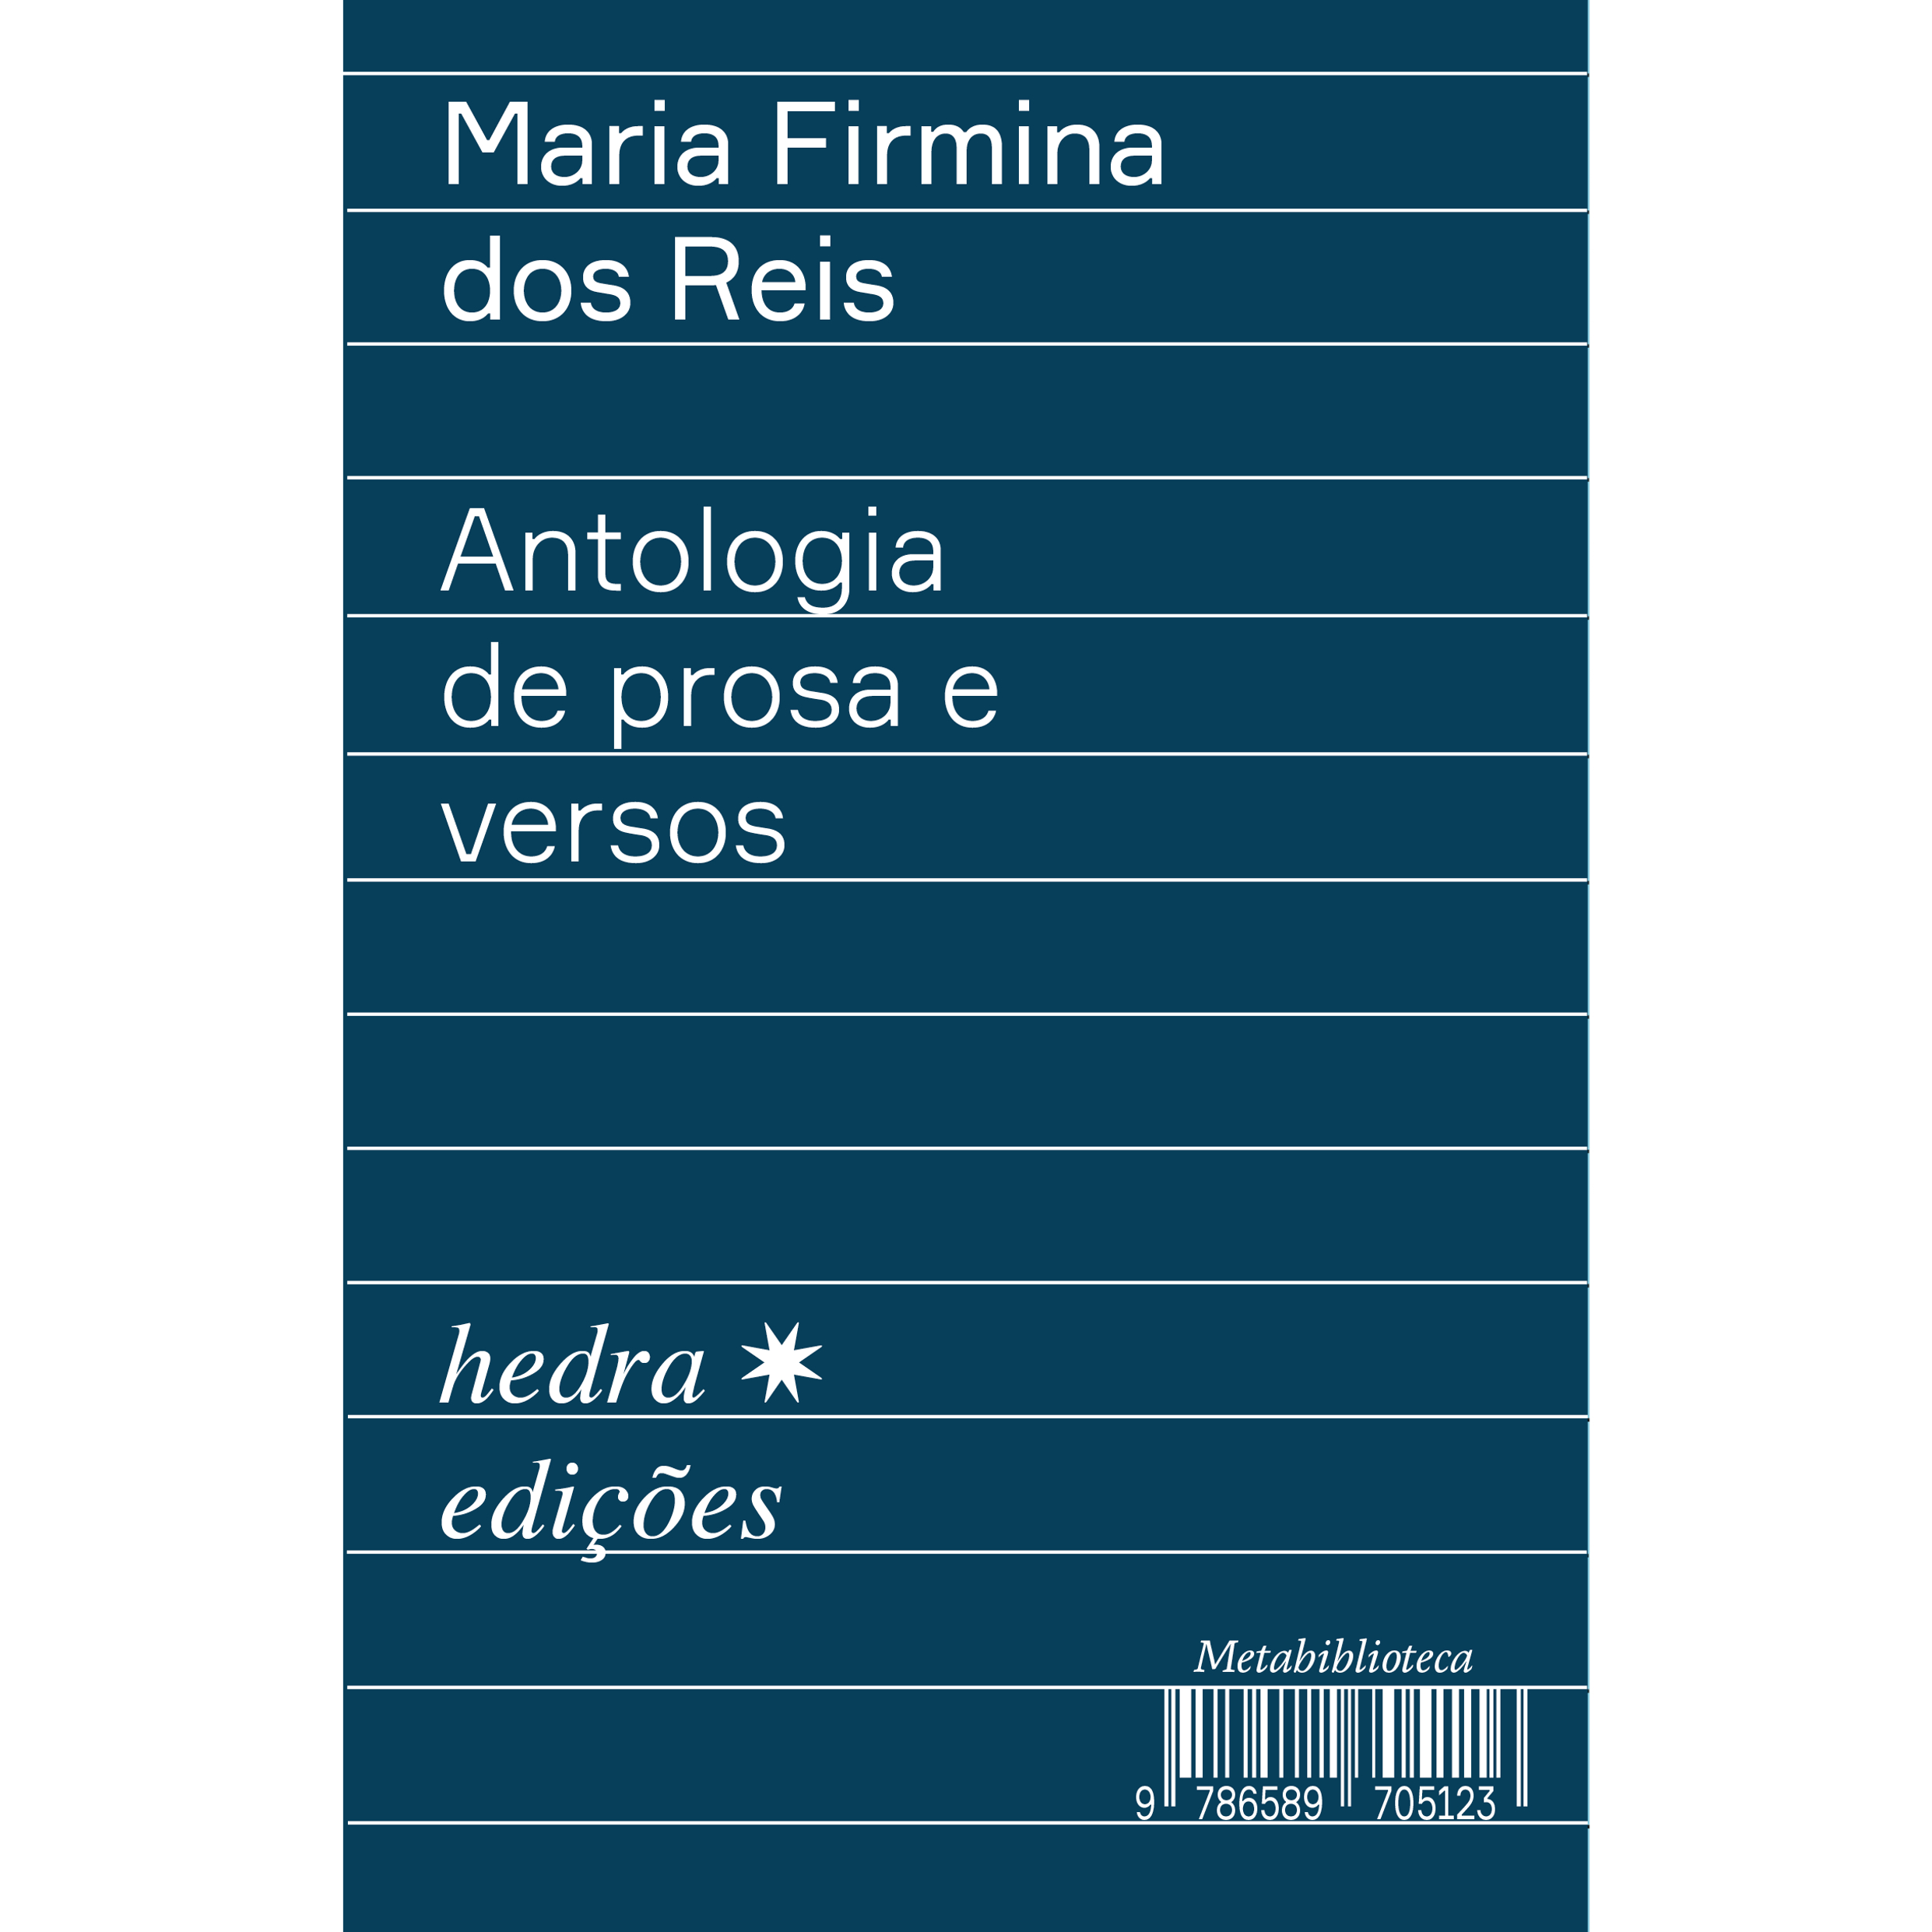
\includegraphics[width=74mm]{./grid/firmina.png}
\end{center}

\hspace*{-7cm}\hrulefill\hspace*{-7cm}

\medskip

\noindent{}\textit{Antologia de prosa e versos} consiste em uma reunião de textos de diversos gêneros de Maria Firmina dos Reis, como o conto ``A escrava'', a novela ``Gupeva'' e poemas extraídos das obras \textit{Cantos à beira-mar} e \textit{Parnaso maranhense}, além de outras coletâneas mais recentes da autora. Nesta antologia, a escritora apresenta alguns dos principais elementos que caracterizam sua literatura, como a condição dos escravizados, que passam a ter protagonismo nas narrativas, o papel da mulher na sociedade, as condições dos povos indígenas, um sentimentalismo romântico amoroso e a exaltação da terra. Maria Firmina dos Reis é considerada a primeira romancista negra da história da literatura brasileira. Além de escritora, foi compositora, musicista e professora primária. Sua obra foi resgatada apenas na segunda metade do século XX.
\vfill

\noindent\begin{minipage}[c]{.5\linewidth}
{\small\textbf{
\hspace*{-.1cm}Editora: Hedra\\
Título: Antologia de prosa e versos\\
Autor: Maria Firmina dos Reis\\ 
%ISBN: 978-65-89705-23-9\\
Páginas: 176\\
Formato: 13,3x21cm\\
Preço: R\$ 68,90\\
}}
\end{minipage}

\pagebreak

\begin{center}
\hspace*{-3.6cm}
\hspace*{3.1cm}
\includegraphics[width=74mm]{./grid/diario.png}
\end{center}

\hspace*{-7cm}\hrulefill\hspace*{-7cm}

\medskip

\noindent{}\textit{Diários de Adão e Eva} é uma espécie de diário íntimo do primeiro casal, dividido em duas partes: ``Fragmentos do diário de Adão'' e ``Diário de Eva'', e os contos ``Solilóquio de Adão'', ``Autobiografia de Eva'' e ``Passagens do diário de Satã''.Os dois primeiros descrevem, do ponto de vista pessoal dos personagens, as novíssimas condições de vida no Paraíso logo após a criação, incluindo as primeiras impressões de Adão sobre a obra divina e sua nova companheira --- e vice-versa. Os contos trazem as experiências da vida depois do Éden e da maturidade --- além das considerações de um observador privilegiado, Satã (reinventado como alguém capaz de ajudar, a partir de sua enorme experiência, o jovem e ingênuo casal). Obra póstuma de um dos maiores escritores e satiristas norte-americanos, pela primeira vez em português.

\vfill

\noindent\begin{minipage}[c]{1\linewidth}
{\small\textbf{
\hspace*{-.1cm}Editora: Hedra\\
Título: Diários de Adão e Eva\\
Autor: Mark Twain\\ 
%ISBN: 978-65-89705-22-2\\
Páginas: 140\\
Formato: 13,3x21cm\\
Preço: R\$ 140,00\\
}}
\end{minipage}

\pagebreak

\begin{center}
\hspace*{-3.6cm}\raisebox{5cm}{\rotatebox[origin=t]{90}{\huge\textbf{Seleção especial}}}
\hspace*{3.1cm}
\includegraphics[width=74mm]{./grid/brown.png}
\end{center}

\hspace*{-7cm}\hrulefill\hspace*{-7cm}

\medskip

\noindent{}William Wells Brown (1814–1884) foi um abolicionista, romancista, dramaturgo e historiador afro-americano. Nascido escravo, fugiu para a liberdade aos 20 anos de idade e, aos 33, publicou esta narrativa. Brown conta a história de sua vida nos estados do Kentucky e Missouri, onde trabalhou como aprendiz em um jornal, no transporte de cativos para a venda em Nova Orleans e em diversas outras atividades. Descreve com riqueza de detalhes os horrores da escravidão, o tráfico negreiro interno nos EUA e a relação com seus donos e familiares.
O autor, no entanto, não hesita em revelar seus vícios e defeitos, destacando assim a individualidade que se desenvolveu sob uma instituição totalizante e desumanizadora, que via em homens e mulheres apenas braços para a lavoura e ventres para uma nova geração de cativos. A \textit{Narrativa de William Wells Brown} é uma crítica à ganância e à hipocrisia religiosa, ao preconceito e à violência, mas, acima de tudo, é uma proclamação da humanidade do seu autor e de todos os que sofreram ao seu lado.

\vfill

\noindent\begin{minipage}[c]{.5\linewidth}
{\small\textbf{
\hspace*{-.1cm}Editora: Hedra\\
Título: Narrativa de William Wells Brown, escravo fugitivo\\
Autor: William Wells Brown\\ 
%ISBN: 978-65-89705-04-8\\
Páginas: 142\\
Formato: 13,3x21cm\\
Preço: R\$ 49,00\\
}}
\end{minipage}

\pagebreak

\begin{center}
\hspace*{-3.6cm}
\hspace*{3.1cm}
\includegraphics[width=74mm]{./grid/harriet.png}
\end{center}

\hspace*{-7cm}\hrulefill\hspace*{-7cm}

\medskip

\noindent{}Nascida na Carolina do Norte por volta do outono de 1813, Harriet Ann Jacobs viveu a tragédia do cativeiro até principiar uma vida em fuga que terminou por levá-la ao Norte em 1842. Foi de Boston que Jacobs conseguiu escrever \textit{Incidentes da vida de uma escrava} que, sem deixar de se inserir no corpus dos relatos da escravidão norte-americana, guarda uma singularidade: é pioneiro e inspirador das autobiografias femininas, e joga luz nos horrores que eram partilhados apenas entre as mulheres cativas.
``A escravidão é terrível para os homens'', escreve a autora, ``mas é muito mais terrível para as mulheres''. Jacobs convive, antes e depois da fuga, com o perverso sistema de assédio e coação sexual contra o qual as escravas procuravam lutar. Transmitindo brilhantemente uma vida em prosa crua e seca, os Incidentes aqui relatados adicionam camadas de complexidade ao horror da escravidão.

\vfill

\noindent\begin{minipage}[c]{1\linewidth}
{\small\textbf{
\hspace*{-.1cm}Editora: Hedra\\
Título: Incidentes da vida de uma escrava\\
Autor: Harriet Ann Jacobs\\ 
%ISBN: 978-65-89705-24-6\\
Páginas: 400\\
Formato: 13,3x21cm\\
Preço: R\$ 99,00\\
}}
\end{minipage}

\pagebreak

\begin{center}
\hspace*{-3.6cm}\raisebox{5cm}{\rotatebox[origin=t]{90}{\huge\textbf{Seleção especial}}}
\hspace*{3.1cm}
\includegraphics[width=74mm]{./grid/nascidos.png}
\end{center}

\hspace*{-7cm}\hrulefill\hspace*{-7cm}

\medskip

\noindent{}Inéditas no país, aqui estão reunidas narrativas de 204 ex-escravizados norte-americanos sobre temas centrais da escravidão nas Américas: cultura negra, resistência, violência, relações familiares durante a escravidão, trabalho, emancipação.
Coletadas através do Projeto Federal de Escritores (FWP), pertencente ao órgão Administração do Progresso no Trabalho (WPA), criado na esteira da Crise de 1929 para garantir a renda de escritores desempregados, as narrativas revelam a memória de milhares de pessoas sobreviventes ao trauma da escravidão. Ao todo, o Projeto Federal de Escritores salvou 2400 narrativas, aproximações de dentro, em perspectiva única, do que foi o escravismo sulista norte-americano, que às vésperas da abolição da escravatura contava com 4 milhões de escravizados em seus campos de trabalho.

\vfill

\noindent\begin{minipage}[c]{1\linewidth}
{\small\textbf{
\hspace*{-.1cm}Editora: Hedra\\
Título: Nascidos na escravidão: depoimentos norte-americanos\\
Autor: Tâmis Parron (Org.)\\ 
%ISBN: 978-65-89705-19-2\\
Páginas: 352\\
Formato: 13,3x21cm\\
Preço: R\$ 99,00\\
}}
\end{minipage}

\pagebreak

\begin{center}
\hspace*{-3.6cm}
\hspace*{3.1cm}
\includegraphics[width=74mm]{./grid/robinson.png}
\end{center}

\hspace*{-7cm}\hrulefill\hspace*{-7cm}

\medskip

\noindent{}O argumento básico de Robinson Crusoé é universalmente conhecido. Isolado em sua \textit{ilha do desespero} após um trágico naufrágio, o marujo inglês luta pela sobrevivência valendo-se de todos os escassos meios a seu alcance. Com o tempo e os utensílios recuperados do navio, chega a se tornar um competente marceneiro e agricultor, além de pastor de cabras e profundo conhecedor da Bíblia --- a única leitura disponível. Sem contato com qualquer ser humano por mais de duas décadas, certo dia Crusoé salva um nativo do assassinato por canibais que haviam aportado numa das praias da ilha, e logo o faz seu criado, dando-lhe o nome de Sexta-Feira. Alguns anos mais tarde, o acaso leva um navio inglês às proximidades da ilha, dando início a um longo conflito com a tripulação amotinada.

\vfill

\noindent\begin{minipage}[c]{1\linewidth}
{\small\textbf{
\hspace*{-.1cm}Editora: Hedra\\
Título: Robinson Crusoé\\
Autor: Daniel Defoe\\ 
%ISBN: 978-65-89705-20-8\\
Páginas: 376\\
Formato: 13,3x21cm\\
Preço: R\$ 129,90\\
}}
\end{minipage}

\pagebreak

\begin{center}
\hspace*{-3.6cm}\raisebox{5cm}{\rotatebox[origin=t]{90}{\huge\textbf{Seleção especial}}}
\hspace*{3.1cm}
\includegraphics[width=74mm]{./grid/ivan.png}
\end{center}

\hspace*{-7cm}\hrulefill\hspace*{-7cm}

\medskip

\noindent{}\textit{A morte de Ivan Ilitch} é uma novela de Lev Tolstói, publicada pela primeira vez em 1886. Considerada uma das obras-primas da literatura, foi escrita logo após sua conversão religiosa do final da década de 1870, em que o velho escritor critica as convenções familistas e as aparências sociais, a superficialidade e a hipocrisia da alta sociedade. Geralmente classificado entre os melhores exemplos de novela, conta a história de um juiz de alta corte e seus sofrimentos e morte por uma doença terminal na Rússia do século XIX.
\vfill

\noindent\begin{minipage}[c]{1\linewidth}
{\small\textbf{
\hspace*{-.1cm}Editora: Hedra\\
Título: A morte de Ivan Ílitch\\
Autor: Lev Tolstói\\ 
%ISBN: 978-65-89705-26-0\\
Páginas: 96\\
Formato: 13,3x21cm\\
Preço: R\$ 43,00\\
}}
\end{minipage}

\pagebreak

\begin{center}
\hspace*{-3.6cm}
\hspace*{3.1cm}
\includegraphics[width=74mm]{./grid/stoker.png}
\end{center}

\hspace*{-7cm}\hrulefill\hspace*{-7cm}

\medskip

\noindent{}\textit{Sob o pôr do sol} inicia com um conto cujo título é justamente ``Sob o Pôr do Sol''. Trata-se de um conto-moldura, que cria uma espécie de quadro geral que estabelece as bases para a leitura dos contos subsequentes. Por meio dessa técnica, Stoker estabelece um fio condutor que alinha todas as narrativas do livro, definindo o espaço e o tempo dos contos. Tanto os contos de Sob o pôr do sol quanto o romance Drácula se estruturam sobre as oposições ``bem e mal'', ``claro e escuro'', ``verdade e mentira'', ``loucura e sanidade''. Caracterizam-se pela forte presença do universo infantil, do moralismo e de valores advindos da religião. \textit{Sob o pôr do sol}, em especial, não obstante ser uma das primeiras obras do autor, revela com grande força a poeticidade de sua prosa, com trechos de grande lirismo e maestria na arte de narrar histórias. A presente tradução buscou ser fiel às nuances do original e à qualidade da linguagem de Stoker e vem a público para mostrar ao leitor brasileiro que o talento de Bram Stoker não se prende a somente uma narrativa.

\vfill

\noindent\begin{minipage}[c]{1\linewidth}
{\small\textbf{
\hspace*{-.1cm}Editora: Hedra\\
Título: Sob o pôr do sol\\
Autor: Bram Stoker\\ 
%ISBN: 978-65-89705-20-8\\
Páginas: 184\\
Formato: 13,3x21cm\\
Preço: R\$ 69,90\\
}}
\end{minipage}

\pagebreak

\begin{center}
\hspace*{-3.6cm}\raisebox{5cm}{\rotatebox[origin=t]{90}{\huge\textbf{Seleção especial}}}
\hspace*{3.1cm}
\includegraphics[width=74mm]{./grid/medico.png}
\end{center}

\hspace*{-7cm}\hrulefill\hspace*{-7cm}

\medskip

\noindent{}\textit{O médico e o monstro} é um dos maiores clássicos do terror psicológico, marcado pelo cientificismo da época vitoriana. O respeitado médico escocês, dr. Jekyll, faz pesquisas para entender os impulsos e os sentimentos humanos mais profundos, a acaba por criar uma droga que libera seus aspectos mais primitivos, o animal adormecido sob a capa do homem civilizado: no seu caso, ele assume a forma de mr. Hyde (do verbo hide, esconder, ocultar; mr. Hyde é a versão oculta do bom dr. Jekyll). Se Jekyll é um médico educado e dedicado a pesquisas que visam o bem-estar geral através do conhecimento, a monstruosidade de Hyde está, essencialmente, em sua entregra aos prazeres e à luxúria como um fim em si, por quaisquer meios, incluindo a força física.O livro influenciou a literatura assim como a cultura pop. Além de inúmeras adaptações para vários meios, como o cinema, é o modelo para personagens de quadrinhos, como o Hulk, a versão furiosa do dr. Banner. Por outro lado, segue uma tradição de ficção psicológica e tecnicista moderna, cujo modelo orginal é o Frankenstein de Mary Shelley.

\vfill

\noindent\begin{minipage}[c]{1\linewidth}
{\small\textbf{
\hspace*{-.1cm}Editora: Hedra\\
Título: O médico e o monstro\\
Autor: Robert Louis Stevenson\\ 
%ISBN: 978-65-89705-25-3\\
Páginas: 114\\
Formato: 13,3x21cm\\
Preço: R\$ 44,00\\
}}
\end{minipage}

\pagebreak


\begin{center}
\hspace*{-3.6cm}
\hspace*{3.1cm}
\includegraphics[width=74mm]{./grid/rashomon.png}
\end{center}

\hspace*{-7cm}\hrulefill\hspace*{-7cm}

\medskip

\noindent{}O livro traz dez contos do grande expoente do conto moderno japonês, publicados entre 1915 e 1927. ``Rashômon'' e ``Dentro do bosque'', retratam a cultura de Heian (atual Quioto), enquanto outros temas explorados por Akutagawa são os antigos costumes japoneses, a ética cristã e a loucura (``Memorando Ryôsai Ogata'', ``Ogin'', ``O mártir''). Já ``Devoção à literatura popular'' e ``Terra morta'' têm como fundo a cultura de Edo (atual Tóquio). Por fim, dois contos de caráter autobiográfico, do final da vida de Akutagawa: ``Passagens do caderno de notas de Yasukichi'' e ``A vida de um idiota''. Esta nova edição, com texto revisto pelas tradutoras, conta ainda com nova introdução e acréscimo de notas.
\vfill

\noindent\begin{minipage}[c]{1\linewidth}
{\small\textbf{
\hspace*{-.1cm}Editora: Hedra\\
Título: Rashômon e outros contos\\
Autor: Akutagawa\\ 
%ISBN: 978-65-89705-20-8\\
Páginas: 208\\
Formato: 13,3x21cm\\
Preço: R\$ 59,00\\
}}
\end{minipage}

\pagebreak


\begin{center}
\hspace*{-3.6cm}\raisebox{5cm}{\rotatebox[origin=t]{90}{\huge\textbf{Seleção especial}}}
\hspace*{3.1cm}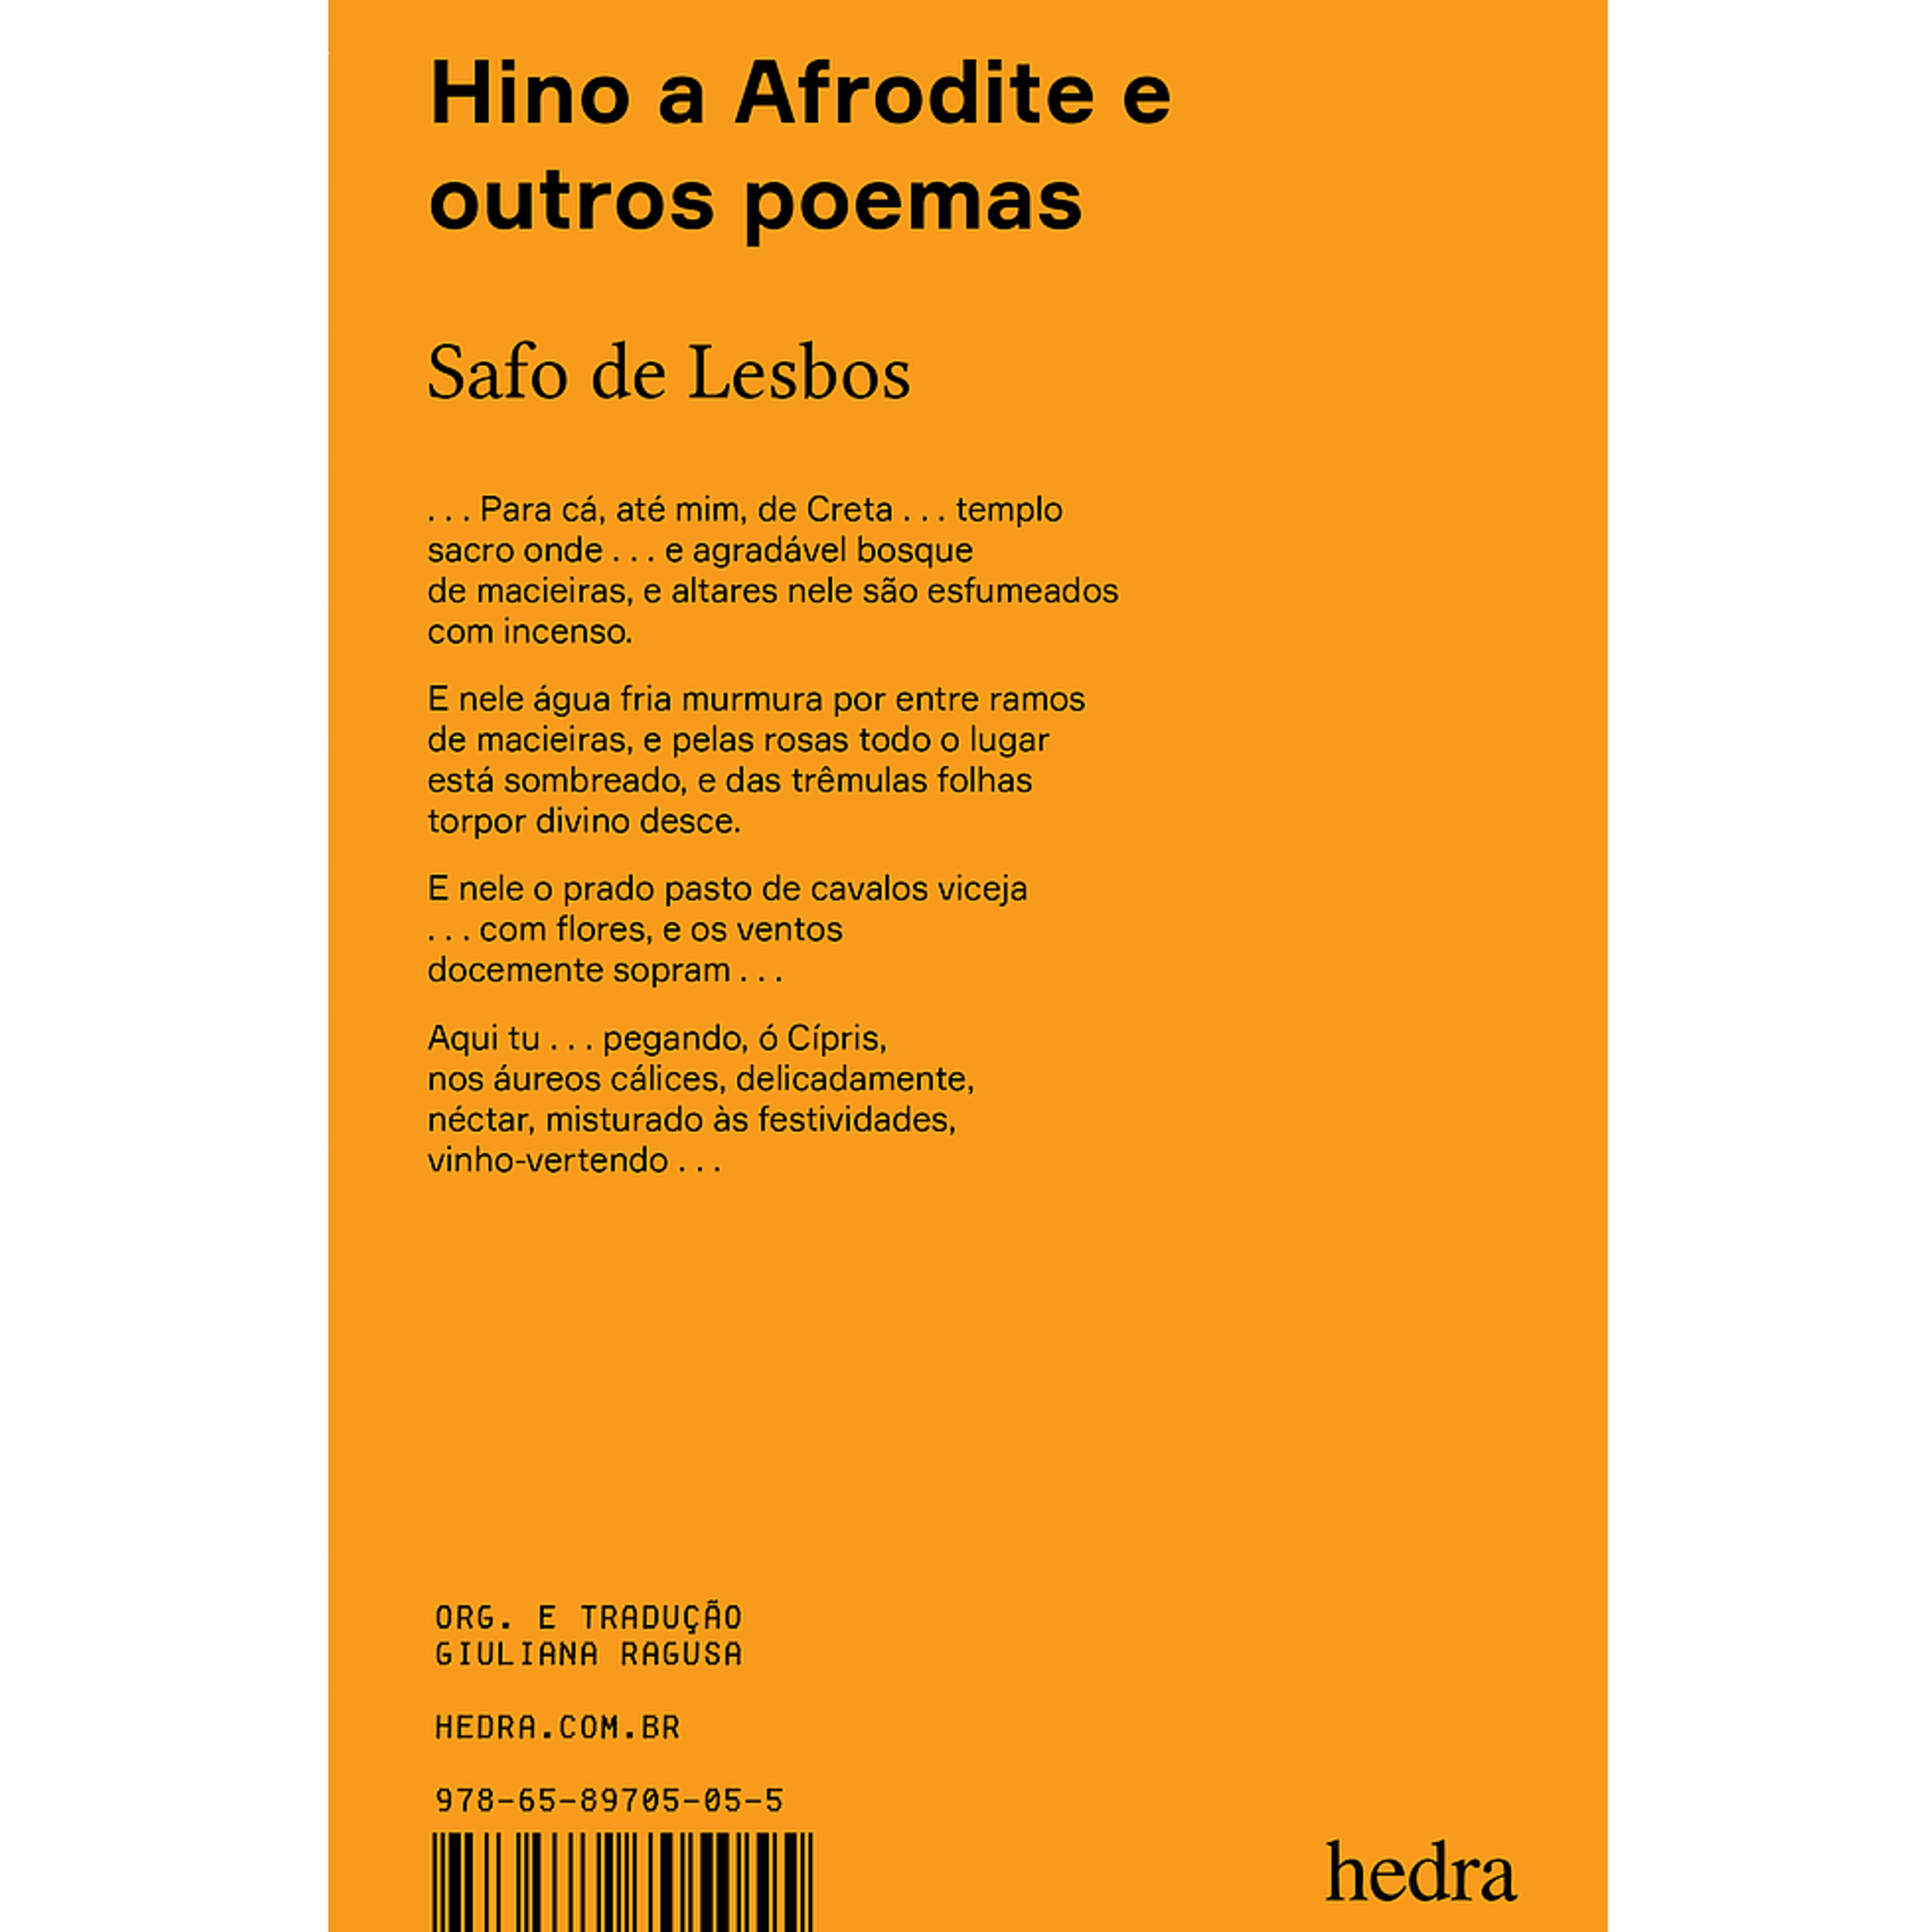
\includegraphics[width=74mm]{./grid/safo.png}
\end{center}

\hspace*{-7cm}\hrulefill\hspace*{-7cm}

\medskip

\noindent{}Reunião de textos remanescentes da mélica de Safo, ou seja, as canções para performance ao som da lira. Os textos aqui são traduzidos e anotados por Giuliana Ragusa em segunda edição --- com novos poemas, atualizações e em versão bilíngue ---, autora que ganhou o Jabuti 2006 com um livro sobre a lírica da poeta, a única mulher entre os grandes da época. Para esta edição foram selecionados a única canção completa e os fragmentos mais legíveis de canções do \textit{corpus} de Safo. As anotações de leitura buscam lançar luz sobre elementos relevantes da estrutura, conteúdo ou transmissão dos fragmentos organizados tematicamente. Precede a tradução anotada uma introdução sobre a poeta, sua poesia e o contexto em que se produziu e circulou, o gênero mélico, a fortuna crítica sobre ela, a transmissão de sua obra, e as outras poetas mulheres de que se tem notícia.

\vfill

\noindent\begin{minipage}[c]{1\linewidth}
{\small\textbf{
\hspace*{-.1cm}Editora: Hedra\\
Título: Hino a Afrodite\\
Autor: Safo de Lesbos\\ 
%ISBN: 978-65-89705-20-8\\
Páginas: 212\\
Formato: 13,3x21cm\\
Preço: R\$ 69,90\\
}}
\end{minipage}

\pagebreak

% \vspace*{1.5cm}

% \noindent{}{\nohyphens{\LARGE{Texto}}}

% \bigskip

% \hfill{}\scalebox{.8}{AUTOR}

% \bigskip
% \bigskip
% \bigskip

% \begin{multicols}{2}
% \noindent{}Mussum Ipsum, cacilds vidis litro abertis. Atirei o pau no gatis, per gatis num morreus. Leite de capivaris, leite de mula manquis sem cabeça. Praesent malesuada urna nisi, quis volutpat erat hendrerit non. Nam vulputate dapibus. Suco de cevadiss, é um leite divinis, qui tem lupuliz, matis, aguis e fermentis.

% Tá deprimidis, eu conheço uma cachacis que pode alegrar sua vidis. Suco de cevadiss deixa as pessoas mais interessantis. In elementis mé pra quem é amistosis quis leo. Quem num gosta di mim que vai caçá sua turmis!

% Viva Forevis aptent taciti sociosqu ad litora torquent. Mauris nec dolor in eros commodo tempor. Aenean aliquam molestie leo, vitae iaculis nisl. Posuere libero varius. Nullam a nisl ut ante blandit hendrerit. Aenean sit amet nisi. Vehicula non. Ut sed ex eros. Vivamus sit amet nibh non tellus tristique interdum.

% Em pé sem cair, deitado sem dormir, sentado sem cochilar e fazendo pose. Detraxit consequat et quo num tendi nada. Pra lá , depois divoltis porris, paradis. Per aumento de cachacis, eu reclamis.

% Quem manda na minha terra sou euzis! A ordem dos tratores não altera o pão duris. Paisis, filhis, espiritis santis. Aenean aliquam molestie leo, vitae iaculis nisl.

% Diuretics paradis num copo é motivis de denguis. Mais vale um bebadis conhecidiss, que um alcoolatra anonimis. Sapien in monti palavris qui num significa nadis i pareci latim. Admodum accumsan disputationi eu sit. Vide electram sadipscing et per.

% Manduma pindureta quium dia nois paga. Interagi no mé, cursus quis, vehicula ac nisi. Praesent vel viverra nisi. Mauris aliquet nunc non turpis scelerisque, eget. Casamentiss faiz malandris se pirulitá.

% Quem num gosta di mé, boa gentis num é. Si num tem leite então bota uma pinga aí cumpadi! Todo mundo vê os porris que eu tomo, mas ninguém vê os tombis que eu levo! Cevadis im ampola pa arma uma pindureta.

% \vspace{\baselineskip}

% {\small\fakereceipt{
% \noindent{}Diuretics paradis num copo é motivis de denguis. Mais vale um bebadis conhecidiss, que um alcoolatra anonimis. Sapien in monti palavris qui num significa nadis i pareci latim. Admodum accumsan disputationi eu sit. Vide electram sadipscing et per.
% }}

% \vspace{\baselineskip}

% Mussum Ipsum, cacilds vidis litro abertis. Atirei o pau no gatis, per gatis num morreus. Leite de capivaris, leite de mula manquis sem cabeça. Praesent malesuada urna nisi, quis volutpat erat hendrerit non. Nam vulputate dapibus. Suco de cevadiss, é um leite divinis, qui tem lupuliz, matis, aguis e fermentis.

% Tá deprimidis, eu conheço uma cachacis que pode alegrar sua vidis. Suco de cevadiss deixa as pessoas mais interessantis. In elementis mé pra quem é amistosis quis leo. Quem num gosta di mim que vai caçá sua turmis!

% Viva Forevis aptent taciti sociosqu ad litora torquent. Mauris nec dolor in eros commodo tempor. Aenean aliquam molestie leo, vitae iaculis nisl. Posuere libero varius. Nullam a nisl ut ante blandit hendrerit. Aenean sit amet nisi. Vehicula non. Ut sed ex eros. Vivamus sit amet nibh non tellus tristique interdum.

% Em pé sem cair, deitado sem dormir, sentado sem cochilar e fazendo pose. Detraxit consequat et quo num tendi nada. Pra lá , depois divoltis porris, paradis. Per aumento de cachacis, eu reclamis.

% Quem manda na minha terra sou euzis! A ordem dos tratores não altera o pão duris. Paisis, filhis, espiritis santis. Aenean aliquam molestie leo, vitae iaculis nisl.

% Diuretics paradis num copo é motivis de denguis. Mais vale um bebadis conhecidiss, que um alcoolatra anonimis. Sapien in monti palavris qui num significa nadis i pareci latim. Admodum accumsan disputationi eu sit. Vide electram sadipscing et per.

% Manduma pindureta quium dia nois paga. Interagi no mé, cursus quis, vehicula ac nisi. Praesent vel viverra nisi. Mauris aliquet nunc non turpis scelerisque, eget. Casamentiss faiz malandris se pirulitá.

% Quem num gosta di mé, boa gentis num é. Si num tem leite então bota uma pinga aí cumpadi! Todo mundo vê os porris que eu tomo, mas ninguém vê os tombis que eu levo! Cevadis im ampola pa arma uma pindureta.

% \bigskip

% \noindent{}\textcolor{gray}{\footnotesize\slsc{\textls[-15]{Texto tal tal e tal.}}}
% \end{multicols}



% \pagebreak
\pagestyle{hedracat}

\begin{multicols}{2}
\begin{enumerate}
\raggedright\nohyphens{
\item Ecopolítica, \textbf{Edson Passetti (org.)}	
\item Mare nostrum: Paranã Tipi, \textbf{Fabio Atui}
\item Crônicas de caça e criação, \textbf{Uirá Garcia}
\item Nas redes guarani, \textbf{Valéria Macedo}
\item A constituição traída, \textbf{Cleonildo Cruz (org.)}
\item Diário de um escritor na Rússia, \textbf{Flávio Ricardo Vassoler}
\item Lugar de negro, lugar de branco?, \textbf{Douglas Rodrigues Barros}
\item A sociedade de controle, \textbf{Sergio Amadeu (org.)}
\item O renascimento do autor, \textbf{Caio Gagliardi}
\item O que eu vi o que nós veremos, \textbf{Santos Dumont}
\item O outro lado da moeda (Teleny), \textbf{Oscar Wilde}
\item Imagens de um mundo trêmulo, \textbf{John Milton}
\item Michel Temer e o fascismo comum, \textbf{Tales Ab'Sáber}
\item Ao longo do rio, \textbf{Alexandre Koji Shiguehara}
\item Solombra, ou a sombra que cai sobre o eu, \textbf{João Adolfo Hansen}
\item Joana d'Arc, \textbf{Jules Michelet}
\item O coletivo aleatório, \textbf{Luis Marra}
\item A história das religiões na cultura moderna, \textbf{Marcello Massenzio}
\item Cordel - F. das Chagas Batista, \textbf{Francisco das Chagas Batista}
\item Elixir do pajé, \textbf{Bernardo Guimarães}
\item Cordel - João Martins de Athayde, \textbf{João Martins de Athayde}
\item Modos de representação da Bienal de São Paulo, \textbf{Vinicius Spricigo}
\item Padeirinho da Mangueira: retrato sincopado de um artista, \textbf{Franco Paulino}
\item Do futuro e da morte do teatro brasileiro, \textbf{Christina Barros Riego}
\item Canudos, história em versos, \textbf{Manuel Pedro das Dores Bombinho}
\item O cego e outros contos, \textbf{D. H. Lawrence}
\item Poesia seiscentista
\item Monoteísmos e dualismos: as religiões da salvação, \textbf{Giovanni Filoramo}
\item Apologia de Galileu, \textbf{Tommaso Campanella}
\item Flor do deserto, \textbf{Waris Dirie; Cathleen Miller}
\item Cinco lugares da fúria, \textbf{Pádua Fernandes}
\item O livro dos mandamentos, \textbf{Maimônides}
\item A conjuração de Catilina, \textbf{Salústio}
\item Fábula de Polifemo e Galatéia e outros poemas, \textbf{Góngora}
\item Histórias de igrejas destruídas, \textbf{Eduardo Brigagão Verderame}
\item Performances, \textbf{Brian Friel}
\item Cultura pop japonesa, \textbf{Sonia Bide Luyten}
\item História trágica do doutor Fausto, \textbf{Christopher Marlowe}
\item Micromegas, \textbf{Voltaire}
\item Politeísmos: as religiões do mundo antigo, \textbf{Paolo Scarpi}
\item Triunfos, \textbf{Petrarca}
\item Museu arte hoje, \textbf{Martin Grossmann; Gilberto Mariotti}
\item Viagem sentimental, \textbf{Laurence Sterne}
\item A Arte de olhar diferente, \textbf{Braulio Tavares}
\item O Pequeno Zacarias chamado Cinábrio, \textbf{E.T.A. Hoffman}
\item Oliver Twist (Bolso), \textbf{Charles Dickens}
\item Alegoria - Construção e interpretação da metáfora, \textbf{João Adolfo Hansen}
\item Teatro do êxtase, \textbf{Fernando Pessoa}
\item Paulo Whitaker, \textbf{Paulo Whitaker}
\item Todas as coisas pequenas, \textbf{Noemi Jaffe}
\item Questão do fim da arte em Hegel, \textbf{Marco Aurélio Werle}
\item Tratados da terra e gente do Brasil, \textbf{Fernão Cardim}
\item Dos nervos, \textbf{Ricardo Lísias}
\item Adeus ponta do meu nariz, \textbf{Edward Lear}
\item Cidade ampliada, \textbf{Rodrigo José Fermino}
\item O diário perdido do Jardim Maia, \textbf{Luís Marra}
\item Sobre a filosofia e outros diálogos, \textbf{Jorge Luis Borges; Osvaldo Ferrari}
\item Cordel: Franklin Maxado, \textbf{Franklin Maxado}
\item Dos novos sistemas na arte, \textbf{Kazimir Malievitch}
\item Cordel: Cuíca de Santo Amaro, \textbf{Cuíca de Santo Amaro}
\item Manual da destruição, \textbf{Alexandre Dal Farra}
\item A imprensa carnavalesca no Brasil, \textbf{José Ramos Tinhorão}
\item Índia e Extremo Oriente: via da libertação e da imortalidade, \textbf{Massimo Raveri}
\item Leitores e leituras de Clarice Lispector
\item Círculos de coca e fumaça, \textbf{Danilo Paiva Ramos}
\item Cordel: Severino José, \textbf{Severino José}
\item Escritório; O Espaço da Produção, \textbf{Claudio Silveira Amaral}
\item As minas de Salomão, \textbf{Rider Haggard}
\item Crédito à morte, \textbf{Anselm Jappe}
\item A cidade e as serras, \textbf{Eça de Queiroz}
\item Oliver Twist, \textbf{Charles Dickens}
\item Dao De Jing, \textbf{Lao Zi}
\item Sobre a amizade e outros diálogos, \textbf{Jorge Luis Borges; Osvaldo Ferrari}
\item Aqui tem coisa, \textbf{Patativa do Assaré}
\item Dicionário livre do santome-português, \textbf{Araújo \& Hagemeijer}
\item Aqui tem coisa, \textbf{Patativa do Assaré}
\item Imagem contemporânea I
\item Cordel - J. Borges, \textbf{José Francisco Borges}
\item Exato acidente, \textbf{Tony Monti}
\item Woyzeck, \textbf{George Buchner}
\item Autobiografia de um super-herói, \textbf{Alexandre Barbosa de Souza}
\item O menino da rosa, \textbf{Tony Monti}
\item Cordel - Rouxinol do Rinaré, \textbf{Rouxinol do Rinaré}
\item Imagem contemporânea II
\item História da província Santa Cruz, \textbf{Pero de Magalhães Gandavo}
\item Édipo Rei, \textbf{Sófocles}
\item Cordel - José Soares, \textbf{José Soares}
\item Greve contra a guerra, \textbf{Ricardo Lísias}
\item Cidade anônima, \textbf{Beatriz Furtado}
\item Primeiro de abril, \textbf{André Luiz Pinto}
\item Cordel: Oliveira de Panelas, \textbf{Oliveira de Panelas}
\item Fazendo Rizoma
\item Uma história do futebol, \textbf{Bill Murray}
\item Gangorra, \textbf{Regina Sawaya}
\item Poesia vaginal, \textbf{Glauco Mattoso}
\item Cultura popular - uma introdução, \textbf{Dominic Strinati}
\item Vocabulário de música pop, \textbf{Roy Shuker}
\item A invenção da pornografia, \textbf{Lynn Hunt}
\item Eu conheci Benny Moré
\item Deriva, \textbf{André Fernandes}
\item Fedro, \textbf{Platão}
\item Sobre os sonhos e outros diálogos, \textbf{Jorge Luis Borges; Osvaldo Ferrari}
\item O sapo voador, \textbf{Ademir Barbosa Jr.}
\item Arcana coelestia e Apocalipsis revelata, \textbf{Emanuel Swedenborg}
\item Letra de forma, \textbf{Laura Estelita Teixeira}
\item Os cães de que desistimos, \textbf{Chantal Castel}
\item Cordel - Téo Azevedo, \textbf{Téo Azevedo}
\item O que eu vi, o que nós veremos [bolso], \textbf{Santos Dumont}
\item A Fábrica de robôs, \textbf{Karel Tchápek}
\item Folhas de relva, \textbf{Walt Whitman}
\item Helio Piñon : Ideias e formas, \textbf{Pfeiffe, Helen; Ana Rosa}
\item O Rabi de Bacherach e três artigos sobre o ódio racial, \textbf{Heinrich Heine}
\item Refugiados de Idomeni, \textbf{Gabriel Bonis}
\item Visão de psicanálise, \textbf{Renato Bulcão}
\item Viagem em volta do meu quarto, \textbf{Xavier de Maistre}
\item Contos clássicos de vampiro, \textbf{Lord Byron; Bram Stoker}
\item Cultura estética e liberdade, \textbf{Friedrich Von Schiller}
\item Dostoiévski e a dialética, \textbf{Flávio Ricardo Vassoler}
\item Cabeças e outros poemas, \textbf{Pedro Luis Marques de Armas}
\item Razão sangrenta, \textbf{Robert Kurz}
\item A Velha Izerguil e outros contos, \textbf{Maksim Górki}
\item Viagem à turquia, bálcãs e Egito, \textbf{John Milton}
\item Do sentimento trágico da vida, \textbf{Miguel de Unamuno}
\item Rashômon e outros contos, \textbf{Akutagawa}
\item Feitiço de amor e outros contos, \textbf{Johann Ludwig Tieck}
\item Ode ao Vento Oeste e outros poemas, \textbf{P. B. Shelley}
\item Esperança do mundo, \textbf{Albert Camus}
\item Universidade, cidade, cidadania, \textbf{Franklin Leopoldo e Silva}
\item Estado crítico, \textbf{Régis Bonvicino}
\item Poemas da cabana montanhesa, \textbf{Saigyo}
\item Dançando em Lúnassa, \textbf{Brian Frield}
\item Lulismo, carisma pop e cultura anticrítica, \textbf{Tales Ab'Sáber}
\item Utopia Brasil, \textbf{Darcy Ribeiro}
\item Americanismo e fordismo, \textbf{Antonio Gramsci}
\item Troca de pele, \textbf{Tereza Yamashita}
\item O Surgimento da noite, \textbf{Pajés Parahiteri}
\item Contos de Sebastopol, \textbf{Liev Tolstói}
\item Um anarquista e outros contos, \textbf{Joseph Conrad}
\item Um Retrato do artista quando jovem, \textbf{James Joyce}
\item O Princípio do Estado e outros ensaios, \textbf{Mikhail Bakunin}
\item A Desmedida na medida, \textbf{Albert Camus}
\item O Chamado selvagem, \textbf{Jack London}
\item O Novo epicuro, \textbf{Edward Sellon}
\item Elogio da loucura, \textbf{Erasmo de Rotterdam}
\item Senhorita Júlia e outras peças, \textbf{August Strindberg}
\item Dublinenses, \textbf{James Joyce}
\item Don Juan ou O convidado de pedra, \textbf{Molière}
\item Manual inútil da televisão, \textbf{Paulo Henrique Amorim}
\item A Vida de Mat, \textbf{Mino Carta}
\item Baleiazzzul, \textbf{Sergio Zlotnic}
\item A Decadência do analfabetismo / A arte de birlibirloque, \textbf{José Bergamín}
\item Balada dos enforcados e outros poemas, \textbf{François Villon}
\item O Médico e o monstro, \textbf{Robert Louis Stevenson}
\item Marco Cornélio Frontão, \textbf{Pascal Quignard}
\item O Casamento do Céu e do Inferno, \textbf{William Blake}
\item O Homem da cabeça de papelão, \textbf{João do Rio}
\item Teleny, ou o reverso da medalha, \textbf{Oscar Wilde}
\item Cordel: Rodolfo Coelho Cavalcante, \textbf{Coelho Cavalcante}
\item Dicionário de História e Cultura da era Viking, \textbf{Johnni Langer}
\item Gente de Hemsö, \textbf{August Strindberg}
\item Viagem aos Estados Unidos, \textbf{Alexis de Tocqueville}
\item Sobre a utilidade e a desvantagem da história para a vida, \textbf{Friedrich Nietzsche}
\item Flossie, a Vênus de quinze anos, \textbf{Charles Swinburne}
\item Os cantos do homem-sombra
\item Escritos revolucionários, \textbf{Errico Malatesta}
\item Micromegas e outros contos, \textbf{Voltaire}
\item Descobrindo o Islã no Brasil, \textbf{Karla Lima}
\item A Cidade mágica, \textbf{Edith Nesbitt}
\item O Alienista, \textbf{Machado de Assis}
\item Cadeira de balanço, \textbf{Vanessa Campos Rocha; Flávio Castellan}
\item Inspiração nordestina, \textbf{Patativa do Assaré}
\item Coisas que a gente gosta e não gosta, \textbf{Laura Teixeira; Fábio Zimbres}
\item A Guerra começou, onde está a guerra?, \textbf{Albert Camus}
\item Poesia completa, \textbf{Orides Fontela}
\item A Volta do parafuso, \textbf{Henry James}
\item Cartas a favor da escravidão, \textbf{José de Alencar}
\item Pequeno-burgueses, \textbf{Maksim Górki}
\item Cordel : Paulo Nunes Batista, \textbf{Paulo Nunes Batista}
\item Esquimó, \textbf{Olivier Douzou}
\item Sai da frente, vaca brava!, \textbf{Ricardo Lísias}
\item Lampião... Era o cavalo do tempo atrás da besta da vida, \textbf{Antônio Klévisson Viana}
\item Cordel: Patativa do Assaré, \textbf{Patativa do Assaré}
\item Ernestine ou o nascimento do amor, \textbf{Stendhal}
\item Filadélfia, lá vou eu!, \textbf{Brian Friel}
\item Sonetos, \textbf{William Shakespeare}
\item Crônicas do crack, \textbf{Luis Marra}
\item Peixinhos, \textbf{Bruno Heitz}
\item A Última folha e outros contos, \textbf{O. Henry}
\item Contos indianos, \textbf{Stéphane Mallarmé}
\item Violência, mas para quê?, \textbf{Anselm Jappe}
\item A Vênus das peles, \textbf{Sacher-Leopold Von Masoch}
\item A Voz dos botequins e outros poemas, \textbf{Paul Verlaine}
\item Poemas, \textbf{Lord Byron}
\item A Pele do lobo e outras peças, \textbf{Artur Azevedo}
\item Explosão - Romance da etnologia, \textbf{Hubert Fichte}
\item Stephen herói, \textbf{James Joyce}
\item Diálogo imaginário entre Marx e Bakunin, \textbf{Maurice Cranston}
\item Nada ainda?, \textbf{Christian Voltz}
\item A Vênus de quinze anos (Flossie), \textbf{Charles Swinburne}
\item Os dentinhos, \textbf{Olivier Douzou}
\item Anarquismo, \textbf{Murray Bookchin}
\item Escritos sobre arte, \textbf{Charles Baudelaire}
\item Deus e o Estado, \textbf{Mikhail Bakunin}
\item Pintura e escrita do mundo flutuante, \textbf{Madalena Hashimoto Cordaro}
\item A Árvore dos cantos, \textbf{Pajés Parahiteri}
\item Poesia catalã - das origens à Guerra Civil
\item Sobre a filosofia e seu método, \textbf{Arthur Schopenhauer}
\item Pensamento político de Maquiavel, \textbf{Johann Fichte}
\item Sobre a ética, \textbf{Arthur Schopenhauer}
\item A Autobiografia do poeta-escravo, \textbf{Juan Francisco Manzano}
\item Cálcio, \textbf{Pádua Fernandes}
\item Bola de sebo e outros contos, \textbf{Guy de Maupassant}
\item Como gente grande, \textbf{Anouk Ricard}
\item O Cavalo de Ébano, \textbf{Richard Burton}
\item Nos cumes do desespero, \textbf{Emil Cioran}
\item A Vênus das peles [Bolso], \textbf{Leopold Von Sacher-Masoch}
\item Homo Pictor, \textbf{Christoph Wulf}
\item 1964
\item Desenganos da vida humana e outros poemas, \textbf{Gregório de Matos}
\item A Nostálgica e outros contos, \textbf{Aléxandros Papadiamántis}
\item Cântico dos Cânticos, \textbf{Salomão}
\item Os Sovietes traídos pelos bolcheviques, \textbf{Rudolf Rocker}
\item Autobiografia de uma pulga, \textbf{Stanislas de Rhodes}
\item Auto da barca do Inferno, \textbf{Gil Vicente}
\item A Monadologia e outros textos, \textbf{Gottfried Leibniz}
\item O Surgimento dos pássaros, \textbf{Pajés Parahiteri}
\item Contos de piratas, \textbf{Arthur Conan Doyle}
\item O Mundo ou tratado da luz, \textbf{René Descartes}
\item Manifesto comunista, \textbf{Karl Marx; Friedrich Engels}
\item Lira grega, \textbf{Giuliana Ragusa}
\item Poesia basca - das origens à Guerra Civil
\item Cordel: Klévisson Viana, \textbf{Klévisson Viana}
\item Discursos ímpios, \textbf{Marquês de Sade}
\item Cordel : Raimundo Santa Helena, \textbf{Raimundo Santa Helena}
\item Primeiro livro dos amores, \textbf{Ovídio}
\item Último reino, \textbf{Pascal Quignard}
\item Da arte de construir, \textbf{Leon Battista Alberti}
\item Frankenstein, \textbf{Mary Shelley}
\item Cordel : Zé Saldanha, \textbf{Zé Saldanha}
\item Dilma Rousseff e o ódio político, \textbf{Tales Ab'Sáber}
\item Saga dos Volsungos, \textbf{Anônimo}
\item Linear G, \textbf{Gilberto Mendonça Teles}
\item Educação e sociologia, \textbf{Émile Durkheim}
\item Histórias com dragões, príncipes e serpentes, \textbf{Vários}
\item História do boi misterioso, \textbf{Leandro Gomes de Barros; Irani Med}
\item Sobre verdade e mentira, \textbf{Friedrich Nietzsche}
\item Sermões 2, \textbf{Antônio Vieira}
\item Lisístrata, \textbf{Aristófanes}
\item Os Americanos, \textbf{Nathaniel Hawthorne; Edgar Allan Poe; Herman Melville}
\item O Sol não espera, \textbf{Marília Castello Branco}
\item O Fim do ciúme e outros contos, \textbf{Marcel Proust}
\item Álcoois, \textbf{Guillaume Apollinaire}
\item A História do planeta azul, \textbf{Andri Snaer Magnason}
\item Entre camponeses, \textbf{Errico Malatesta}
\item Ispinho e Fulô, \textbf{Patativa do Assaré}
\item Mais dia menos dia, a paixão, \textbf{Nelson de Oliveira}
\item Teogonia, \textbf{Hesíodo}
\item Ação e percepção nos processos educacionais do corpo em formação, \textbf{Cecília Noriko Ito Saito}
\item Amores e outras imagens, \textbf{Filóstrato}
\item O Fantástico reparador de feridas, \textbf{Brian Friel}
\item Mangá, \textbf{Sonia Bide Luyten}
\item Inferno, \textbf{August Strindberg}
\item Romanceiro cigano, \textbf{Sermões}
\item Sagas, \textbf{August Strindberg}
\item O Destino do erudito, \textbf{Johann Fichte}
\item Diários de Adão e Eva, \textbf{Mark Twain}
\item Habitar, \textbf{André Fernandes}
\item O Desertor, \textbf{Silva Alvarenga}
\item Os Vínculos, \textbf{Giordano Bruno}
\item O Estranho caso do Dr. Jekyll e Mr. Hyde, \textbf{Robert Louis Stevenson}
\item Sátiras, fábulas, aforismos e profecias, \textbf{Leonardo da Vinci}
\item Poesia espanhola - das origens à Guerra Civil
\item Hino a Afrodite e outros poemas, \textbf{Safo de Lesbos}
\item Revolução e liberdade, \textbf{Mikhail Bakunin}
\item Cartas do Brasil, \textbf{Antonio Vieira}
\item A Mulher que virou Tatu
\item Sermões 1, \textbf{Antônio Vieira}
\item Fé e saber, \textbf{G.W. Friedrich Hegel}
\item Negras tormentas, \textbf{Alexandre Samis}
\item Cordel: Manoel Caboclo, \textbf{Manoel Caboclo}
\item Graciliano Ramos e A Novidade, \textbf{Ieda Lebensztayn}
\item Emília Galotti, \textbf{Gotthold Ephraim Lessing}
\item Dao De Jing, \textbf{Lao Zi}
\item Histórias escondidas, \textbf{Odilon Moraes}
\item Noites egípcias e outros contos, \textbf{Aleksandr Púchikin}
\item Carmilla, a vampira de Karnstein, \textbf{Sheridan Le Fanu}
\item O desafio de Lula, \textbf{Mino Carta; Gianni Carta}
\item A Filosofia na era trágica dos gregos, \textbf{Friedrich Nietzsche}
\item O Que é bom, o que é ruim, \textbf{Vladimir Maiakóvski}
\item Em busca do Japão contemporâneo, \textbf{John Milton}
\item A Vida de H.P. Lovecraft, \textbf{S.T. Joshi}
\item A Demanda do Santo Graal, \textbf{Anônimo}
\item Trabalhos e os dias, \textbf{Hesíodo}
\item Mensagem, \textbf{Fernando Pessoa}
\item Ode sobre a melancolia e outros poemas, \textbf{John Keats}
\item O Corno de si próprio e outros contos, \textbf{Marquês de Sade}
\item Hawthorne e seus musgos, \textbf{Herman Melville}
\item Memórias de um menino judeu do Bom Retiro, \textbf{Victor Nussenzwieg}
\item No coração das trevas, \textbf{Joseph Conrad}
\item Émile e Sophie ou os solitários, \textbf{Jean-Jaqcques Rousseau}
\item Investigação sobre o entendimento humano, \textbf{David Hume}
\item Ideias de canário, \textbf{Machado de Assis}
\item Eu acuso! / O processo do capitão Dreyfus, \textbf{Émile Zola; Rui Barbosa}
\item O Livro dos dragões, \textbf{Ovídio}
\item As Bacantes, \textbf{Eurípides}
\item Contos clássicos de vampiro [Bolso], \textbf{Lord Byron; Bram Stoker}
\item Sobre a liberdade, \textbf{Stuart Mill}
\item Metamorfoses, \textbf{Ovídio}
\item O Primeiro Hamlet, \textbf{William Shakespeare}
\item O Corvo, \textbf{Claudio Weber Abramo}
\item A Vida é sonho, \textbf{Calderón de La Barca}
\item Eu, \textbf{Augusto dos Anjos}
\item Cordel: Zé Vicente, \textbf{Zé Vicente}
\item Escritos sobre literatura, \textbf{Sigmund Freud}
\item Dez poemas da vizinhança vazia, \textbf{Iuri Pereira}
\item Um gato Indiscreto e outros contos, \textbf{Saki}
\item Ciclovia, \textbf{Ulisses Garcez}
\item O Livro de Monelle, \textbf{Marcel Schwob}
\item A Fábrica de robôs [Bolso], \textbf{Karel Tchápek}
\item Oração aos moços, \textbf{Rui Barbosa}
\item A Metamorfose, \textbf{Franz Kafka}
\item História de Aladim e a lâmpada maravilhosa, \textbf{Patativa do Assaré}
\item Ninfas, \textbf{Giorgio Agamben}
\item O Ladrão honesto e outros contos, \textbf{Fiódor Dostoiévski}
\item O Enigma Orides, \textbf{Gustavo de Castro}
\item A Cruzada das crianças / Vidas imaginárias, \textbf{Marcel Schwob}
\item Sobre o riso e a loucura, \textbf{Hipócrates}
\item Notas sobre o anarquismo, \textbf{Noam Chomsky}
\item Mare Nostrum, \textbf{Fabio Atui}
\item Cordel: Expedito Sebastião Da Silva, \textbf{Expedito Sebastião}
\item Mistério na zona sul, \textbf{Roberto Barbato Junior}
\item Cordel: Zé Melancia, \textbf{Zé Melancia}
\item Lulismo, carisma pop e cultura anticrítica, \textbf{Tales Ab'Sáber}
\item Perversão, \textbf{Robert J. Stoller}
\item Poesia galega - das origens à Guerra Civil
\item Naqueles morros, depois da chuva, \textbf{Edival Lourenço}
\item Os Comedores de terra, \textbf{Pajés Parahiteri}
\item Ilíada, \textbf{Homero}
\item A Semente e a torre, \textbf{Leonardo da Vinci}
\item A Farsa de Inês Pereira, \textbf{Gil Vicente}
\item Cão, \textbf{Rafael Mantovani}
\item Diário de um escritor (1873), \textbf{Fiódor Dostoiévski}
\item Carta sobre a tolerância, \textbf{John Locke}
\item Anarquia pela educação, \textbf{Élisée Reclus}
\item A Raposa sombria, \textbf{Sjón}
\item Anjos do universo, \textbf{Einar Már Gudmundsson}
\item O Indivíduo, a sociedade e o Estado e outros ensaios, \textbf{Emma Goldman}
\item A terra uma só, \textbf{Timóteo da Silva Verá Tupã Popyguá}
\item Mistério no morro do deleite, \textbf{Roberto Barbato Junior}
\item A arte de contar histórias, \textbf{Water Benjamin}
}
\end{enumerate}
\end{multicols}

\pagebreak

%\pagestyle{n-1}
\label{n-1}

%\begin{textblock*}{5.625in}(0pt,0pt)%
%\vspace*{-3.5cm}
%\hspace*{-2.77cm}\includegraphics*[width=175.2mm]{./propagandas/N-1.pdf}
%\end{textblock*}

%\pagebreak %RIOT PUSSY
%
%\begin{center}
%
%\hspace*{.5cm}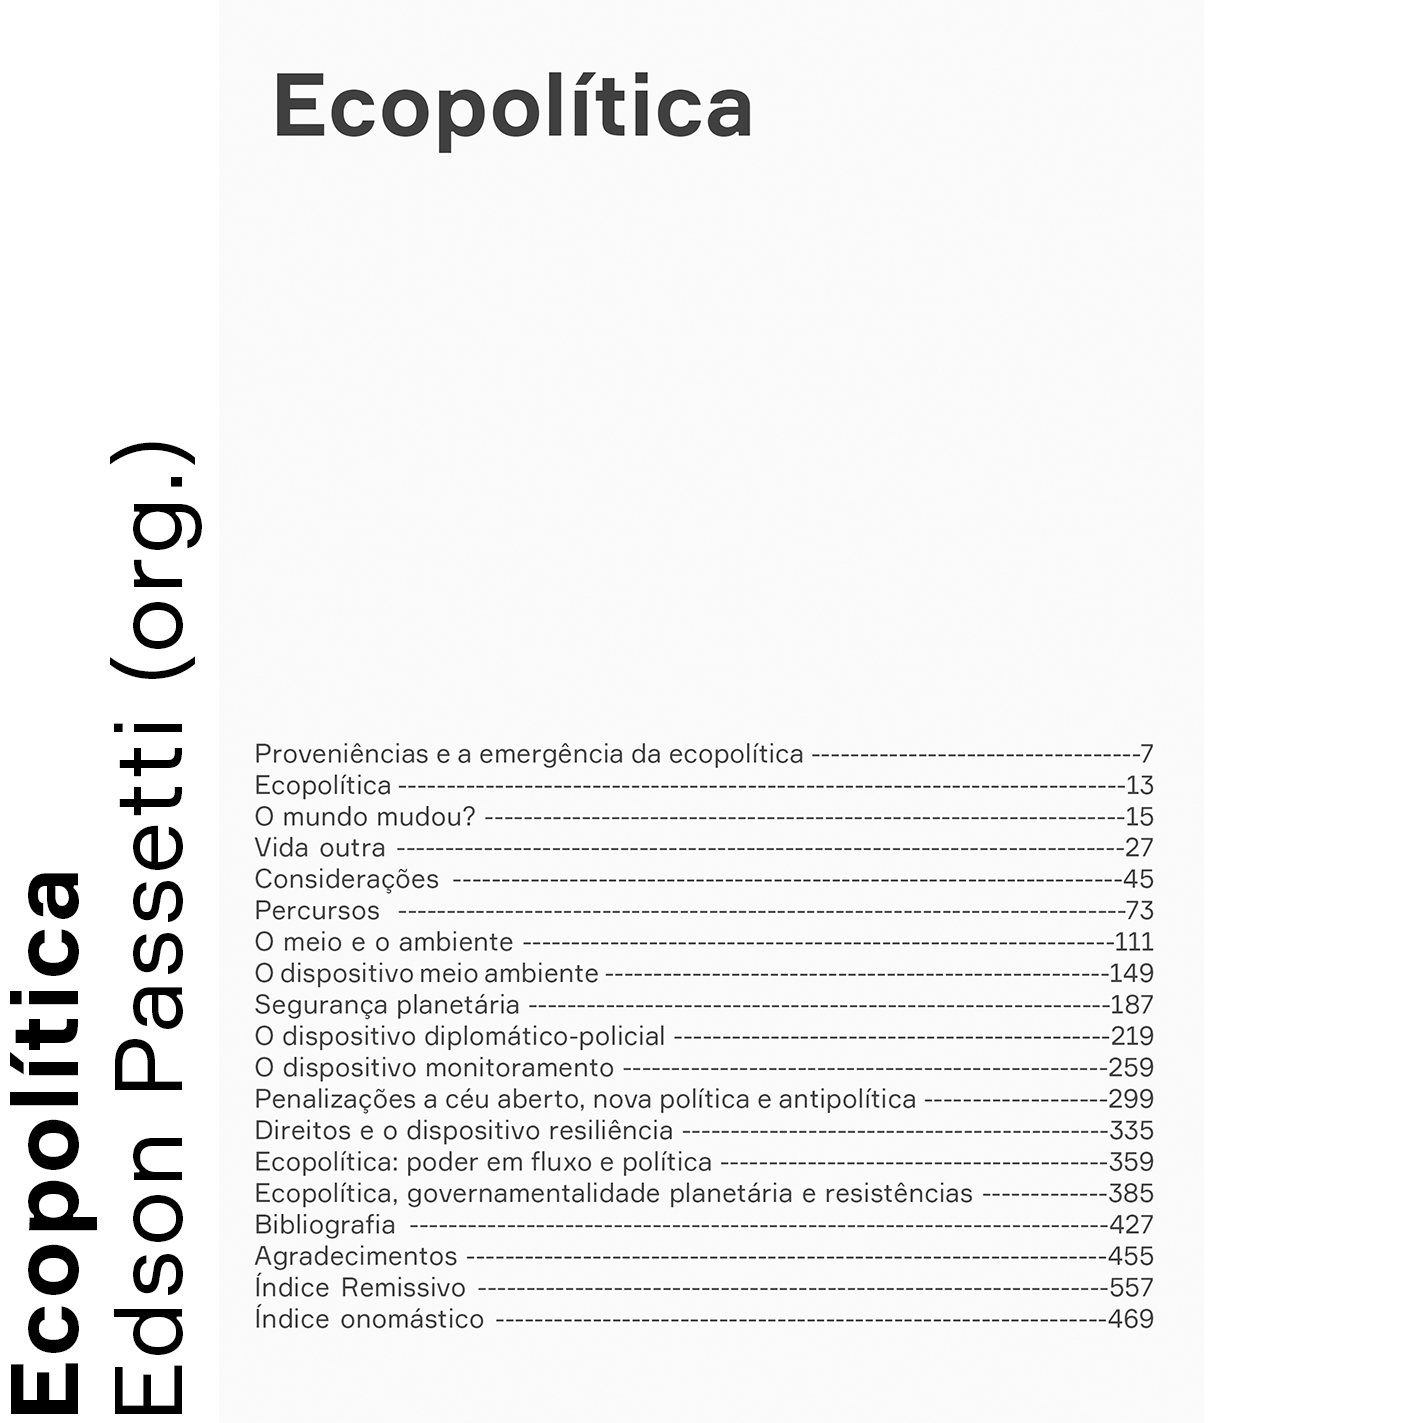
\includegraphics[width=74mm]{./grid/passetti.jpeg}
%\end{center}
%
%\hspace*{-7cm}\hrulefill\hspace*{-7cm}
%
%\medskip
%
%\noindent{}\lipsum[1]
%
%\vfill
%
%\hspace*{-.4cm}\begin{minipage}[c]{.5\linewidth}
%\small\textbf{
%\hspace*{-.1cm}Editora: n-1\\
%Título: Direito de sequência esquizoanalítica (ePub)\\
%Autor: Antoine Sibertin-Blanc\\ 
%ISBN: XXX-XX-XXXX-XXX-X\\
%%Páginas: 216\\
%%Formato: 14x21cm\\
%Preço: R\$ XX,XX\\
%}
%\end{minipage}

%\pagebreak %CORPOS QUE IMPORTAM, JUDITH BUTLER


%\begin{center}
%\hspace*{.5cm}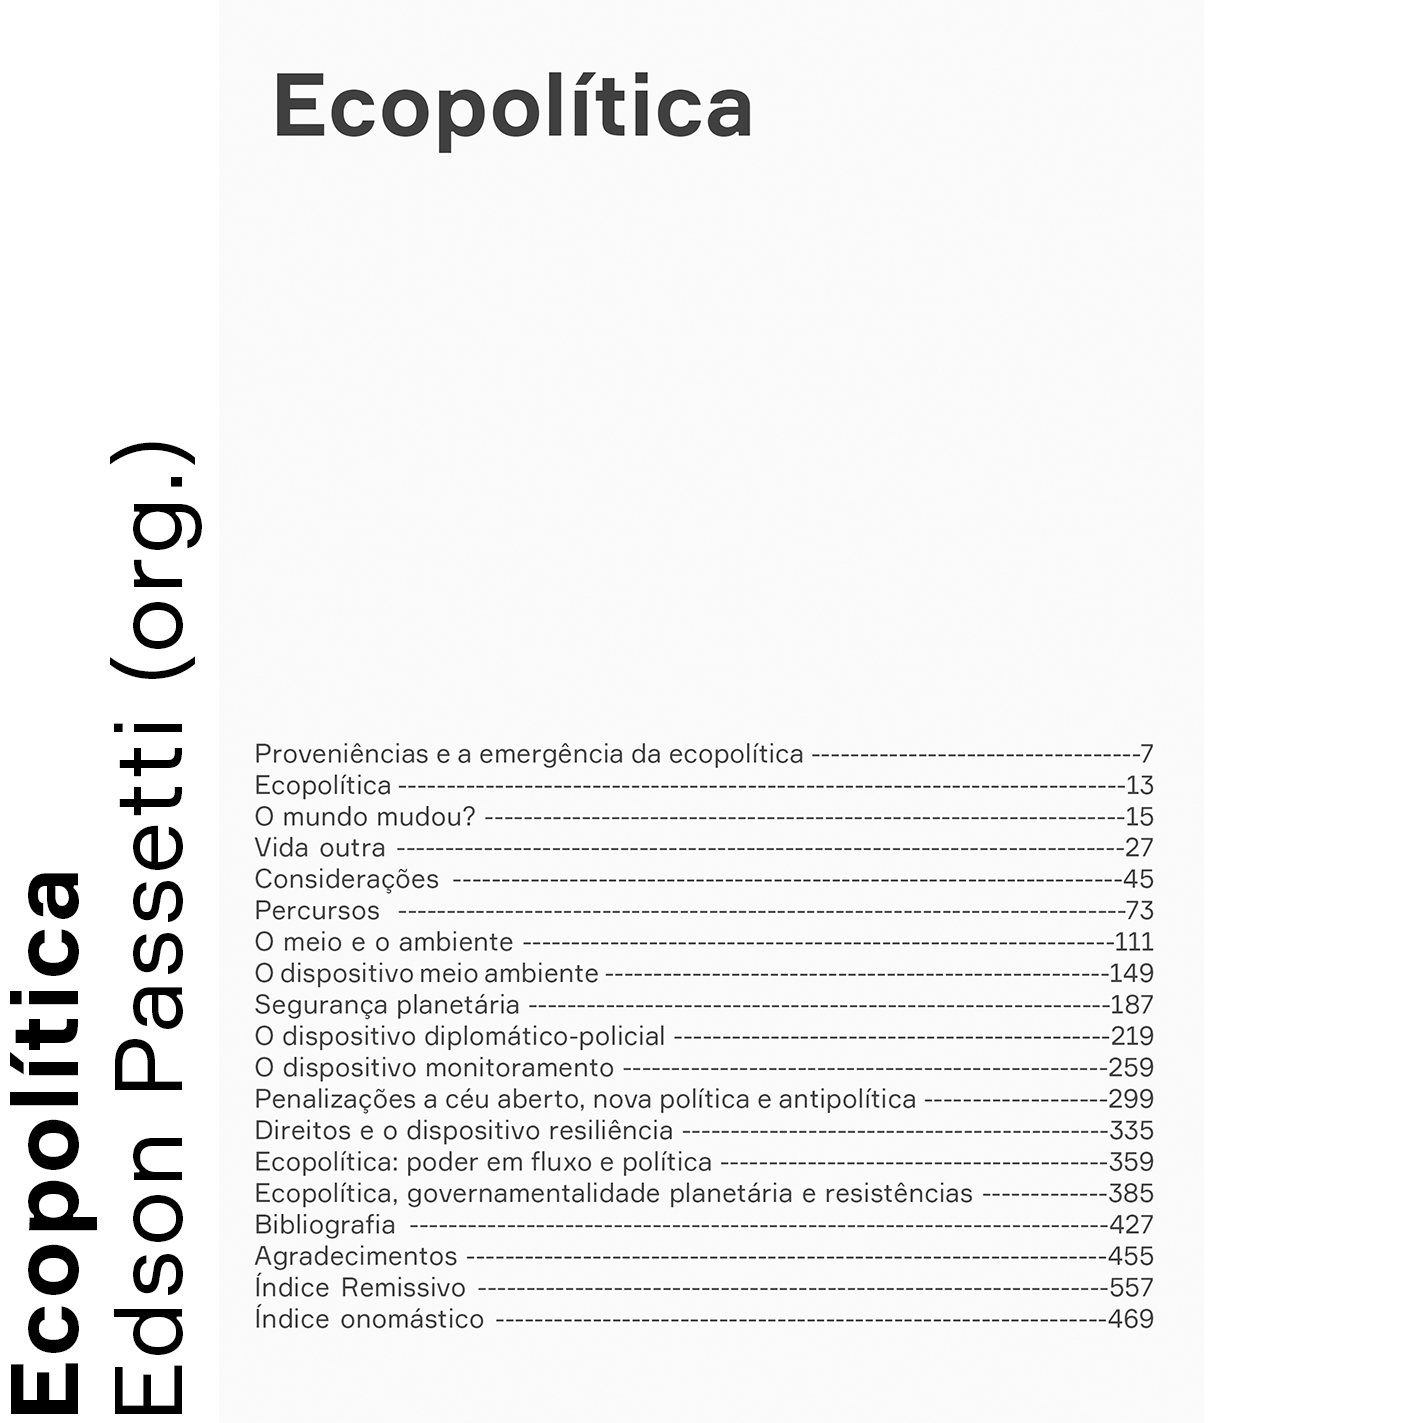
\includegraphics[width=74mm]{./grid/passetti.jpeg}
%\end{center}
%
%\hspace*{-7cm}\hrulefill\hspace*{-7cm}
%
%\medskip
%
%\noindent{}“O propósito deste livro é contribuir, a partir da África, onde vivo e
%trabalho (mas também a partir do resto do mundo, que eu nunca deixei de
%percorrer), para \hlc{uma crítica do tempo que é o nosso --- o tempo do
%repovoamento e da globalização do mundo sob a égide do militarismo e do
%capital e, como consequência derradeira, o tempo da saída da democracia}
%(ou de sua inversão). Para levar este projeto a bom termo, seguiremos
%uma abordagem transversal, atenta aos três motivos da abertura, da
%travessia e da circulação. Uma abordagem dessas só dará frutos se abrir
%espaço para uma \emph{leitura retroativa} do nosso presente.”
%
%
%\vfill
%
%\hspace*{-.4cm}\begin{minipage}[c]{1\linewidth}
%\small\textbf{
%\hspace*{-.1cm}Editora: n-1\\
%Título: Políticas da inimizade\\
%Autor: Achille Mbembe\\ 
%ISBN: 978-65-86941-17-3\\
%Páginas: 216\\
%Formato: 14x21cm\\
%Preço: R\$ XX,XX\\
%}
%\end{minipage}

\pagebreak


\begin{center}
\hspace*{.5cm}\includegraphics[width=74mm]{./grid/porno.jpg}
\end{center}

\hspace*{-7cm}\hrulefill\hspace*{-7cm}

\medskip

\noindent{}É a partir das relações entre arquitetura, tecnologia e sexualidade que \hlc{Paul Preciado aborda o império Playboy, primeira indústria de entretenimento sexual do capitalismo global}. Com um raro talento filosófico, inspirado na ideia de heterotopia de Michel Foucault, o autor inventa a noção de pornotopia, e se debruça sobre o arquipélago Playboy para entendê"-lo como realização contemporânea das utopias sexuais de Sade e tantos outros.


\vfill

\hspace*{-.4cm}\begin{minipage}[c]{1\linewidth}
\small\textbf{
\hspace*{-.1cm}Editora: n-1\\
Título: Pornotopia\\
Autor: Paul B. Preciado\\ 
ISBN: 978-65-86941-23-4\\
Páginas: 228\\
Formato: 14x21cm\\
Preço: R\$ 75,00\\
}
\end{minipage}

\pagebreak %PRAGMATISMO PULSIONAL


\begin{center}
\hspace*{-3.6cm}\raisebox{5cm}{\rotatebox[origin=t]{90}{\huge\textbf{Lançamento}}}
\hspace*{3.1cm}\includegraphics[width=74mm]{./grid/mishima.jpg}
\end{center}

\hspace*{-7cm}\hrulefill\hspace*{-7cm}

\medskip

\noindent{}O dia 25 de novembro de 1970 ficou marcado pelo seppuku do escritor Yukio Mishima no Quartel General Ichigaya de Tokyo, na presença de seus companheiros da Sociedade do Escudo --- Tatenokai. Mais do que o acontecimento em si, há uma certa concepção de corpo e de terrorismo estético que reverbera na obra deste grande escritor. \hlc{O livro \textit{Intoxicações Poéticas da Carne}, do artista brasileiro Gal Oppido, mergulha neste universo ambíguo e subversivo de Mishima criando novas imagens a partir das noções de sacrifício, homoerotismo, dor e prazer.} Há um palimpsesto de gestos que atravessam a imagem do Imperador, devaneios de Sade, o corpo sacrificado de Hijikata e tantas outras cenas que mudaram as nossas vidas.

\vfill

\hspace*{-.4cm}\begin{minipage}[c]{.8\linewidth}
\small\textbf{
\hspace*{-.1cm}Editora: n-1\\
Título: Intoxicações poéticas da carne\\
Autor: Christine Greiner e Gal Oppido\\ 
ISBN: 978-65-86941-20-3\\
Páginas: 176\\
Formato: 17,5x25cm\\
Preço: R\$ 100,00\\
}
\end{minipage}

%\pagebreak %FASCISMO OU REVOLUÇÃO? MAURICIO LAZZARATO
%
%
%\begin{center}
%\hspace*{-3.6cm}\raisebox{5cm}{\rotatebox[origin=t]{90}{\huge\textbf{Lançamento}}}
%\hspace*{3.1cm}\includegraphics[width=74mm]{./grid/mirror.jpg}
%\end{center}
%
%\hspace*{-7cm}\hrulefill\hspace*{-7cm}
%
%\medskip
%
%\noindent{}“Para além de Black Mirror” explora cinco episódios da série televisiva homônima para desenvolver complexas questões que o presente nos força a pensar. São pontos de partida para o desdobramento de reflexões urgentes: as implicações das práticas de aprovação e exclusão em uma cultura de \emph{likes}; a disseminação de linchamentos virtuais por contágios de agressividade em redes sociais, expressando"-se também na emergência de políticos explicitamente caricatos; a dificuldade de lidar com frustrações, perdas e morte, expressa, por exemplo, na promessa de paraísos hedonistas virtuais e de novos corpos sintéticos e imortais. \hlc{Entrecruzando Nietzsche, Gabriel Tarde, Henri Bergson, Deleuze e outros, esse livro embaralha os tempos e se projeta no extemporâneo, com força intempestiva frente às perplexidades que a história não cessa %de provocar.}
%
%\vfill
%
%\hspace*{-.4cm}\begin{minipage}[c]{1\linewidth}
%\small\textbf{
%\hspace*{-.1cm}Editora: n-1\\
%Título: Para além de Black Mirror: Estilhaços distópicos do presente\\
%Autor: Maria Cristina Franco Ferraz e Ericson Saint Clair\\ 
%ISBN: 978-65-86941-12-8\\
%Páginas: 180\\
%Formato: 11x18cm\\
%Preço: R\$ XX,XX\\
%}
%\end{minipage}

\pagebreak %HOMO INC.ORPORATED


\begin{center}
\hspace*{.5cm}\includegraphics[width=74mm]{./grid/homo.jpg}
\end{center}

\hspace*{-7cm}\hrulefill\hspace*{-7cm}

\medskip

\noindent{}\hlc{“Este livro é, entre outras coisas, a história de duas experiências políticas.} A primeira, que eu teria evitado e nunca teria imaginado: o inferno esquisito no qual se transformou a faculdade neoliberal \textit{à la française}, alto lugar da \textit{educastração}, da gestão do pensamento e das subjetividades, especialmente para minorias sexuais, de gênero e raciais; a segunda, o encontro com o coletivo queer e transfeminista italiano de Bolonha, o Smaschieramenti, que me transformou na hora certa.”

\vfill

\hspace*{-.4cm}\begin{minipage}[c]{.5\linewidth}
\small\textbf{
\hspace*{-.1cm}Editora: n-1\\
Título: Homo Inc.Orporated\\
Autor: Sam Bourcier\\ 
ISBN: 978-65-8694-101-2\\
Páginas: 284\\
Formato: 14x21cm\\
Preço: R\$ 65,00\\
}
\end{minipage}

\pagebreak %FERNANDO PESSOA


\begin{center}
\hspace*{-3.6cm}\raisebox{5cm}{\rotatebox[origin=t]{90}{\huge\textbf{Lançamento}}}
\hspace*{3.1cm}\includegraphics[width=74mm]{./grid/pessoa.jpg}
\end{center}

\hspace*{-7cm}\hrulefill\hspace*{-7cm}

\medskip

\noindent{}José Gil toma como matricial de todo esse processo, um alguém atenta para as mínimas sensações intersticiais que lhe sobrevêm, sensações estas tomadas como ondas transportadoras de outras sensações que se lhes associam, sensações transformadas em arte, que são também sensações de um outro, múltiplo gerador de outros. \hlc{“Escrever poemas”, diz José Gil, “é escrever segundo a lógica da heteronímia, é iniciar um processo de devir"-outro que deverá necessariamente levar à produção poética dos heterônimos''}. Sentir"-se outro, ser outro desde o primeiro ato poético da sensação, implica fazer"-se \textit{poeticamente} outros. E só existirão os heterônimos, esses outros, porque cada um deles já é outro para si mesmo, e participando todos de um vertiginoso jogo caleidoscópico. 

\vfill

\hspace*{-.4cm}\begin{minipage}[c]{.5\linewidth}
\small\textbf{
\hspace*{-.1cm}Editora: n-1\\
Título: Fernando Pessoa, ou a Metafísica das sensações\\
Autor: José Gil\\ 
ISBN: 978-65-8694-111-1\\
Páginas: 240\\
Formato: 16x23cm\\
Preço: R\$ 69,00\\
}
\end{minipage}

\pagebreak

\begin{center}
\hspace*{.5cm}\includegraphics[width=74mm]{./grid/queer.jpg}
\end{center}

\hspace*{-7cm}\hrulefill\hspace*{-7cm}

\medskip

\noindent{}Como uma rede formal (uma que, digamos, poderia ser nomeada como ré num processo judicial) \textit{Bash Back!} com certeza está morta. Como adorável terrorista tanto da direita cristã quanto da esquerda \textit{queer}, é claro que nunca existiu fora de um espetáculo. \hlc{Como uma tendência teórica, os pressupostos centrais no cerne de \textit{Bash Back!} continuam a florescer – \textit{queer negation, gender mutiny, not yr cister, baedan, filth and glitter, outlaw bodies} – muitos receptáculos e máscaras em prol de um compromisso invariável e implacável com o que é negativo e rebelde no coração da \textit{queeridade}.} Como conjunto de táticas de gangue, a \textit{Bash Back!} continua viva, sem dúvida. Mesmo quando fazemos o trabalho de antologia, nossa tarefa é incessantemente proliferada: mais viados abrindo no meio crânios de nazistas, mais \textit{queers} se rebelando simplesmente pela alegria de se rebelar, outra igreja atacada, ume jornalista desnorteade relatando sobre uma gangue \textit{queers} particularmente violenta no centrão da cidade.

\vfill

\hspace*{-.4cm}\begin{minipage}[c]{.5\linewidth}
\small\textbf{
\hspace*{-.1cm}Editora: n-1 \& Crocodilo\\
Título: Bash Back -- Ultra violência queer\\
ISBN: 978-65-86941-22-7\\
Páginas: 176\\
Formato: 12x19cm\\
Preço: R\$ 40,00\\
}
\end{minipage}

\pagebreak


\begin{center}
\hspace*{-3.6cm}\raisebox{5cm}{\rotatebox[origin=t]{90}{\huge\textbf{Lançamento}}}
\hspace*{3.1cm}\includegraphics[width=74mm]{./grid/fausto.jpg}
\end{center}

\hspace*{-7cm}\hrulefill\hspace*{-7cm}

\medskip

\noindent{}\textit{A cosmopolítica do animais} é, ao mesmo tempo, a mais importante contribuição filosófica brasileira aos \textit{animal studies} e uma obra ímpar de filosofia política. \hlc{Ao colocar a \textit{pólis}, em suas diversas configurações históricas, sob a perspectiva dos animais não humanos, Juliana Fausto abre um novo horizonte cósmico para a imaginação política}. Entretecendo com maestria fatos, histórias, experiências, conceitos e ideias hauridas das mais variadas fontes, a autora nos faz experimentar um mundo (por vir?) em que nós humanos teremos finalmente nos tornado concidadãos de nossas “espécies companheiras”.

\vfill

\hspace*{-.4cm}\begin{minipage}[c]{.5\linewidth}
\small\textbf{
\hspace*{-.1cm}Editora: n-1\\
Título: A cosmopolítica do animais\\
Autor: Juliana Fausto\\ 
ISBN: 978-65-86941-15-9\\
Páginas: 355\\
Formato: 14x21cm\\
Preço: R\$ 60,00\\
}
\end{minipage}

\pagebreak

\vspace*{1.5cm}

\noindent{}{\nohyphens{\LARGE{O que é a cosmopolítica dos animais?}}}

\bigskip

\hfill{}\scalebox{.8}{JULIANA FAUSTO}

\bigskip
\bigskip
\bigskip

\begin{multicols}{2}
\noindent{}``O homem é, por natureza, um animal político'', a célebre sentença de
Aristóteles constitui não apenas um dos fundamentos de sua teoria
política, mas um dos pilares do pensamento ocidental. Houve, e há,
defensores e detratores da ideia, mas ela é, se não inescapável,
profundamente influente. Os quatro termos da frase remetem a conceitos
complexos que suscitam disputa em relação a seu significado: homem,
natureza, animal e política. Além disso, estão conjugados de modo que
encerram questões que permanecem matéria de debate --- o homem é ou não
um animal, possui ou não uma natureza, é determinado por ela ou a
determina, a política é ou não natural, e o que quer dizer natureza ou
natural nesses contextos, entre outros pontos. Por esses e outros
problemas entrelaçados, tais como os de justiça, lei, direitos,
propriedade e formas de governo, o que se chama de filosofia política
parece ter se fixado exclusivamente no homem.

``Que o homem é um animal político em maior medida que todas as abelhas
e todos os animais de bando é claro'', continuava o filósofo grego. É
que, para ele, só o homem possuiria \emph{lógos} --- discurso, razão,
linguagem ---, o mais fundamental dos muitos avatares da distinção humana
que o pensamento ocidental produziu em sua história. Os animais, sempre
os outros diante dos quais a humanidade se eleva singularmente, além de
desprovidos de linguagem, razão, alma, ferramentas e incontáveis
propriedades, restaram sem política. \emph{Homo homini lupus}, a máxima
evocada por Thomas Hobbes, aponta para a condição

\vspace{\baselineskip}

{\small\fakereceipt{
\noindent{}“Interessam"-me, sobretudo, a situação dos animais outros que humanos e as
políticas concretas, possíveis e experimentais que os capturam, ativam,
oprimem ou são compostas com eles.”
}}

\vspace{\baselineskip}

\noindent{}bruta e bestial das
cidades em sua relação entre si, isto é, sem um Estado dos Estados que
as ordene. Sem essa autoridade superior, onde não se encontra um
mestre, retornar"-se"-ia ao estado de natureza, aquele dos lobos
considerados canibais, configuração sumamente apolítica. No debate
político, os animais surgem apenas como metáforas, símbolos --- lobos,
leões, ratos, cobras, cordeiros etc. --- que significam certas
disposições ou ânimos sem, no entanto, se referirem aos bichos e suas
populações.

Atualmente, o campo conhecido como estudos animais, que reverbera um
interesse renovado por esses outros viventes que dividem o planeta com a
humanidade, tentacularizando"-se em disciplinas de humanidades como
filosofia, literatura, antropologia, história e outras, também começa a
delinear uma teoria política animal. Volumes recentemente lançados
procuram tornar políticas questões de direito ou ética animal por meio
de sua institucionalização. O caminho seguido por este livro afasta"-se
dessa abordagem por não acreditar que política indique apenas o âmbito
das instituições políticas nas formas"-Estado. Pelo contrário, pretendo
procurar definições de política ou práticas políticas que envolvam
criativamente os animais, configurações políticas possíveis
coconstituídas.~Não desejo, com isso, abandonar o campo prático de ação,
mas investir nele em alianças cuja proeminência não seja a de
instituições humanas que, ademais, foram construídas por exclusão dos
animais. Tampouco busco a reunião ou produção de normas e diretrizes,
pois os caminhos são tão múltiplos quanto o são os modos de coabitar o
mundo pelas incontáveis populações animais (inclusive as de animais
humanos). Não se trata, portanto, de um trabalho sobre ética ou de uma
teoria política animal advinda deste, mas do deslocamento do sentido do
que se chama política. Em suma, o objetivo é traçar linhas e caminhos
que devolvam a política ao mundo e seus seres.

Interessam"-me, sobretudo, a situação dos animais outros que humanos e as
políticas concretas, possíveis e experimentais que os capturam, ativam,
oprimem ou são compostas com eles. Seja pela perda de habitat e modos de
vida, pela categorização como animais de companhia, pestes, escravos,
cobaias ou trabalhadores, nos imensos campos em que são mantidos
confinados, pela reprodução forçada, pela morte impedida e pelo
extermínio, os animais estão implicados e são atores numerosos e
potentes nas histórias e estórias que tecemos hoje, no começo do século
\textsc{xxi}, sob o signo do capitalismo liberal, na época geológica chamada
Antropoceno. É diante deles e com eles que procuro construir este texto.
Para tanto, procuro responder à exortação da filósofa ecofeminista Val
Plumwood de que devemos ser capazes de ``pensar diferentemente'', talvez
a única saída possível face à destruição atual: ``Esqueçam o modelo da
máquina passiva e nos contem mais sobre as capacidades autoinventivas e
autoelaborativas da natureza, sobre a intencionalidade do mundo não
humano.'' Se a ``mansão
das liberdades modernas repousa sobre uma base de uso de combustíveis
fósseis em permanente expansão'', e, eu acrescentaria, sobre a opressão de uma infinidade
de entes humanos e outros que humanos, e se esse movimento nos trouxe
até um momento de perigo e devastação, é preciso começar a pensar de
outro modo. Ou, antes, é preciso levar a sério a exortação de Virginia
Woolf, retomada por Donna Haraway: ``Think we must! We must
think.''

\vspace{\baselineskip}

{\small\fakereceipt{
\noindent{}“Convencida de que somente através de
encontros multiespecíficos com outros situados é possível urdir
políticas cósmicas e não exterministas, proponho um mergulho nos olhos
de alguns animais outros que humanos.”
}}

\vspace{\baselineskip}

Hannah Arendt, que inspira Haraway em seu estímulo ao pensamento --- e à
falta de pensamento que leva até a banalidade do mal ---, escreveu que
``pensar com a mentalidade alargada significa treinar a própria
imaginação a sair em visita''. Retiro propositalmente sua frase do contexto
original, profundamente ligado ao cosmopolitismo kantiano etno e
antropocêntrico, e a remeto à seguinte conclamação de Plumwood:
``Libere sua mente e faça suas próprias contribuições ao projeto de
interrupção do reducionismo e do mecanicismo. Ajude"-nos a reimaginar o
mundo em termos mais ricos que nos permitirão nos encontrar em diálogo
com e limitados pelas necessidades de outras espécies, outros tipos de
mentes. Não lhes direi como fazê"-lo. Há muitos modos de fazê"-lo. Mas
espero que os tenha convencido de que este não é um projeto diletante.
\emph{A luta para pensar diferentemente, para refazer nossa cultura
reducionista, é um projeto básico de sobrevivência em nosso presente
contexto}. Espero que vocês se juntem a ele''.

Não tenho nenhuma ilusão quanto ao que posso fazer aqui, algo
infinitamente mais modesto do que pedia Plumwood. Gostaria de pensar,
entretanto, que o espírito destas páginas vem pelo menos tangenciar essa
enorme tarefa.~Para tanto, visito algumas situações conceituais e
experimento modos de relação nos quais os animais outros que humanos
tenham a oportunidade de, existindo politicamente, ajudar a pensar de
modo diferente e a efetivamente cultivar em conjunto, para usar a
expressão de Anna Tsing, ``artes de viver em um mundo danificado''. Como
princípio, procuro sempre me referir a questões situadas, com animais
humanos e outros que humanos determinados, sejam eles povos, indivíduos
ou personagens, seguindo a indicação de Haraway que, inspirada por
Marilyn Strathern, afirma que: 
``Importa quais histórias contamos para contar histórias; importa quais
nós atam nós, quais pensamentos pensam pensamentos, quais descrições
descrevem descrições, quais vínculos vinculam vínculos. Importa quais
histórias fazem mundos, quais mundos fazem histórias''.

Pretendo, assim, escapar àquilo que Jacques Derrida chamou de o
filosofema, o discurso que toma abstratamente os animais outros que
humanos como uma imensa categoria de seres indistintos e que não se
permite ser visto por eles, entrar em relação com eles. Pensar de modo
diferente não pode supor a elaboração do animal como ``um
\emph{teorema}, uma coisa vista mas que não vê''.

Para tanto, privilegiarei algumas configurações concretas da vida dos
animais no Antropoceno, como sua existência em cidades nas feições de
\emph{pets} e errantes, o confinamento ao qual são submetidos em
zoológicos, as experimentações nas quais são parceiros ou cobaias, nas
artes e nas ciências, e a sua desaparição pelos processos acelerados de
extinção. O método utilizado no exame dessas situações envolveu a
abordagem conjunta da filosofia com diferentes discursos, como a
etologia, a biologia, a antropologia, a história e a literatura, na
convicção de que o estudo das políticas animais exige um esforço
conceitual multidisciplinar.

Tais passos não se pretendem nem poderiam ser exaustivos, dada a
profusão imaginativa da vida animal, capaz de inventar novos mundos e
modos de habitá"-los politicamente mesmo diante das opressões mais
abjetas. Se pensar é mesmo um modo de visitar, ao tomar este princípio
como método, acredito tê"-lo feito com a companhia de uma miríade de
autoras e autores; os visitados, por seu turno, não foram os animais em
geral ou a animalidade enquanto categoria; eles têm nomes, como Bruxo,
Batatinha, Nausicaa, Tibbles, Nikkie, Yeroen, Mama, Tushi, Luit, Consul,
Sultão, Rotpeter, Kluger Hans, Mohammed, Zarif, Martha e George e fazem
parte de povos tão diversos e múltiplos quanto o dos gatos, cães, bois e
vacas, cotovias"-da"-ilha"-stephen, galinhas, fragatas, cavalos, gorilas,
chimpanzés, macacos"-rhesus, macacos"-aranha, lobos, OncoRato™,
camundongos, ratos"-pretos e candangos, babuínos, pombos"-passageiros,
formigas, alalas e dingos. Convencida de que somente através de
encontros multiespecíficos com outros situados é possível urdir
políticas cósmicas e não exterministas, proponho um mergulho nos olhos
de alguns animais outros que humanos, na esperança de que, de dentro das
trevas anunciadas pelo Antropoceno, esta ``festa universal da morte,
{[}\ldots{}{]} perniciosa febre que ao nosso redor inflama o céu desta noite
chuvosa'', uma centelha que
divise caminhos enlameados formados por rastros de bichos, possa
porventura brilhar.


\noindent{}\textcolor{gray}{\footnotesize\slsc{Trecho adaptado do livro Cosmopolítica dos animais”.}}
\end{multicols}


\pagebreak
\pagestyle{n-1cat}

\begin{multicols}{2}
\begin{enumerate}
\raggedright\nohyphens{
\item Potências do tempo, \textbf{David Lapoujade}
\item Declaração, \textbf{Antonio Negri; Michael Hardt}
\item Manifesto contrassexual, \textbf{Beatriz Preciado}
\item O aracniano e outros textos, \textbf{Fernand Deligny}
\item Deleuze, os movimentos aberrantes, \textbf{David Lapoujade}
\item Aos nossos amigos, \textbf{Comitê Invisível}
\item Teoria King Kong, \textbf{Virginie Despentes}
\item Guattari: Confrontações / Conversas com Kuniichi Uno e Laymert Garcia dos Santos
\item Quando e como eu li Foucault, \textbf{Antonio Negri}
\item O avesso do niilismo, \textbf{Peter Pál Pelbart}
\item A missão, \textbf{Heiner Müller}
\item William James, a construção da experiência, \textbf{David Lapoujade}
\item Nietzsche -- O bufão dos deuses, \textbf{Maria Cristina Franco Ferraz}
\item Impressões de Michel Foucault, \textbf{Roberto Machado}
\item Fabulações do corpo japonês, \textbf{Christine Greiner}
\item As existências mínimas, \textbf{David Lapoujade}
\item Hegel e o Haiti, \textbf{Susan Buck-Morss}
\item Brazuca, negão e sebento, \textbf{Jean-Christophe Goddard}
\item Motim e destituição agora, \textbf{Comitê Invisível}
\item Crítica da razão negra, \textbf{Achille Mbembe}
\item Testo junkie, \textbf{Paul B. Preciado}
\item O universo inacabado, \textbf{Mario Novello}
\item Cartas e outros textos, \textbf{Gilles Deleuze}
\item Nietzsche e a filosofia, \textbf{Gilles Deleuze}
\item Hijikata tatsumi, \textbf{Kuniichi Uno}
\item Spartakus, \textbf{Furio Jesi}
\item Agamben: por uma ética da vergonha e do resto, \textbf{Oswaldo Giacóia Junior}
\item UPP -- A redução da favela em três letras, \textbf{Marielle Franco}
\item Cinco dias em março, \textbf{Toshiki Okada}
\item Os vagabundos eficazes, \textbf{Fernand Deligny}
\item O enigma da revolta, \textbf{Michel Foucault}
\item Arqueofeminismo
\item Contribuição para a guerra em curso, \textbf{Tiqqun}
\item Ética bixa, \textbf{Paco Vidarte}
\item Ensaios do assombro, \textbf{Peter Pál Pelbart}
\item Metafísicas canibais, \textbf{Eduardo Viveiros de Castro}
\item O governo do homem endividado, \textbf{Maurizio Lazzarato}
\item Leituras do corpo no Japão, \textbf{Christine Greiner}
\item Pragmatismo pulsional, \textbf{João Perci Schiavon}
\item Ruptura, \textbf{Centelha}
\item Às voltas com Lautréamont, \textbf{Laymert Garcia dos Santos}
\item Afrotopia, \textbf{Felwine Sarr}
\item Fascismo ou revolução?, \textbf{Maurizio Lazzarato}
\item Corpos que importam, \textbf{Judith Butler}
\item Somos nosso cérebro?, \textbf{Francisco Ortega; Fernando Vidal}
\item Ritornelos, \textbf{Félix Guattari}
\item Contracultura, entre a curtição e o experimental, \textbf{Celso Favarett}
\item Necropolítica, \textbf{Achille Mbembe}
\item Esferas da inssureição: notas para uma vida não cafetinada, \textbf{Suely Rolnik}

}
\end{enumerate}
\end{multicols}

\pagebreak
%\pagestyle{circuito}
\label{circuito}

%\begin{textblock*}{5.625in}(0pt,0pt)%
%\vspace*{-3.49cm}
%\hspace*{-2.76cm}\includegraphics*[width=175.2mm]{./propagandas/CIRCUITO.pdf}
%\end{textblock*}

%\pagebreak %AS ARTES DO COVER


\begin{center}
\hspace*{.5cm}\includegraphics[width=74mm]{./grid/maciel.jpg}
\end{center}

\hspace*{-7cm}\hrulefill\hspace*{-7cm}

\medskip

\noindent{}São quase verbetes. Katia Maciel reúne \hlc{entrevistas e textos curtos escritos sobre experiências propostas por artistas que expandem ideias de cinema na arte, e procuram acompanhar o circuito de arte contemporânea}. O que explica a
razão pela qual a maioria dos trabalhos analisados ter sido vista em museus
e galerias cariocas, embora um ou outro tenha sido visitado em outros
estados e países. São muitas as questões que os artistas colocam à forma
clássica do cinema como um dispositivo de exibição de imagens em
movimento para um público sentado diante de um fio de luz. Apropriação,
arquivo, registro, dispositivo, máquina, diálogo, fotografia, tecnologia, escala,
memória, fabulação, performance, tempo, outras tecnologias e modos de ver,
novas interlocuções com o espectador visitante. Termos e relações que
redefinem a experiência cinema.

\vfill

\hspace*{-.4cm}\begin{minipage}[c]{1\linewidth}
\small\textbf{
\hspace*{-.1cm}Editora: Circuito\\
Título: A ideia de cinema na arte contemporânea brasileira\\
Autor: Katia Maciel\\ 
ISBN: 978-65-8697-404-01\\
Páginas: 110\\
Formato: 14x21cm\\
Preço: R\$ 40,00\\
}
\end{minipage}

\pagebreak %TODOS OS LUGARES


\begin{center}
\hspace*{-3.6cm}\raisebox{5cm}{\rotatebox[origin=t]{90}{\huge\textbf{Lançamento}}}
\hspace*{3.1cm}\includegraphics[width=74mm]{./grid/noite.jpg}
\end{center}

\hspace*{-7cm}\hrulefill\hspace*{-7cm}

\medskip

\noindent{}\hlc{A Romênia, sob o jugo do ditador Nicolae Ceausescu, atravessa um dos piores períodos da sua história, com a população a enfrentar a fome e dominada pelo terror.} Seguindo as orientações do Presidente para a criação de um exército do povo no qual os soldados seriam treinados desde crianças, Paul, um ambicioso funcionário do partido, decide levar de casa o filho de três anos e entregá-lo aos cuidados do Estado. Quando a mãe se apercebe do desaparecimento do pequeno Drago, o desespero já não a abandonará,
bem como o firme desejo de acabar com a vida do marido. Correndo riscos tremendos,
Nadia não desistirá, porém, de procurar o menino, ainda que para isso tenha de forjar
uma nova identidade, de fazer falsas denúncias, de correr os orfanatos cujas imagens
terríveis chocaram o mundo e até de integrar uma rede que transporta clandestinamente
crianças romenas soropositivas para o Ocidente. Mas será que o seu sofrimento pode
ser apaziguado enquanto Paul for vivo? Enquanto o ditador for vivo?

\vfill

\hspace*{-.4cm}\begin{minipage}[c]{1\linewidth}
\small\textbf{
\hspace*{-.1cm}Editora: Circuito\\
Título: A noite não é eterna\\
Autor: Ana Cristina Silva\\ 
ISBN: 978-65-8697-404-1\\
Páginas: 130\\
Formato: 16x23cm\\
Preço: R\$ 39,90\\
}
\end{minipage}

\pagebreak

\begin{center}
\hspace*{.5cm}\includegraphics[width=74mm]{./grid/asas.jpg}
\end{center}

\hspace*{-7cm}\hrulefill\hspace*{-7cm}

\medskip

\noindent{}A intensidade da narrativa prende desde a primeira linha. \hlc{Densa, mas fluente, misto de poesia, filosofia, biografia imaginária, compensadora na intertextualidade que convoca outras leituras.} Começa com a história de Gabriel, Clara e Florimundo, o filho. E não por acaso, o espaço inicial é o de um mundo fechado, onde Gabriel escreve uma obra literária sem fim.

\vfill

\hspace*{-.4cm}\begin{minipage}[c]{1\linewidth}
\small\textbf{
\hspace*{-.1cm}Editora: Circuito\\
Título: Asas de Saturno\\
Autor: Maria João Cantinho\\ 
ISBN: 978-65-8697-406-5\\
Páginas: 128\\
Formato: 16x23cm\\
Preço: R\$ 39,90\\
}
\end{minipage}

\pagebreak %INTRODUÇÃO À SOMA

\begin{center}
\hspace*{-3.6cm}\raisebox{5cm}{\rotatebox[origin=t]{90}{\huge\textbf{Lançamento}}}
\hspace*{3.1cm}\includegraphics[width=74mm]{./grid/impunidade.jpg}
\end{center}

\hspace*{-7cm}\hrulefill\hspace*{-7cm}

\medskip

\noindent{}Uma estranha beleza, melancólica, nimba de luz estas personagens. Não é exagero se dissermos, como o autor o diz, no final do livro, que ela irradia do “esplendor das coisas ameaçadas”, como a beleza dos condenados, nos romances de Kafka. \hlc{Essa é a linhagem de H. G. Cancela, o negrume de Dostoiévski ou de Thomas Bernard. O mundo em que a escrita tem o poder de dar a ver o lado mais obscuro do humano}, sem ilusões falseadoras, gesto ético e de fidelidade última.

\vfill

\hspace*{-.4cm}\begin{minipage}[c]{1\linewidth}
\small\textbf{
\hspace*{-.1cm}Editora: Circuito\\
Título: Impunidade\\
Autor: H.G. Cancela\\ 
ISBN: 978-65-8697-405-8\\
Páginas: 190\\
Formato: 16x23cm\\
Preço: R\$ 53,00\\
}
\end{minipage}

\pagebreak

\begin{center}
\hspace*{.5cm}\includegraphics[width=74mm]{./grid/quartos.jpg}
\end{center}

\hspace*{-7cm}\hrulefill\hspace*{-7cm}

\medskip

\noindent{}Nove contos sobre espaços que são nossos durante um período limitado para depois	regressarem ao domínio público, ou serem tomados por um novo ocupante temporário.
\hlc{O leitor pode esperar uma profusão de gestos, manobras, frases e movimentações de
mobília destinados a tornar quartos e apartamentos menos anônimos.} Os exageros
--- reescrever na íntegra um clássico da teoria da religião comparada, defender que um
quarto no Campo de Santa Clara deu outrora guarida a um poeta russo prestes a cair
em desgraça, celebrar a memória de suicidas parisienses) --- são, nestas circunstâncias,
desculpáveis.


\vfill

\hspace*{-.4cm}\begin{minipage}[c]{1\linewidth}
\small\textbf{
\hspace*{-.1cm}Editora: Circuito\\
Título: Quartos alugados\\
Autor: Alexandre Andrade\\ 
ISBN: 978-65-8697-403-4\\
Páginas: 144\\
Formato: 16x23cm\\
Preço: R\$ 42,90\\
}
\end{minipage}



\pagebreak

\begin{center}
\hspace*{-3.6cm}\raisebox{5cm}{\rotatebox[origin=t]{90}{\huge\textbf{Lançamento}}}
\hspace*{3.1cm}\includegraphics[width=74mm]{./grid/conversas.jpg}
\end{center}

\hspace*{-7cm}\hrulefill\hspace*{-7cm}

\medskip

\noindent{}\textit{Conversas transversais com Yuri Firmeza} apresenta a reunião de mais de uma década de textos produzidos com e a partir dos trabalhos do Yuri, sobre suas ações e sua inserção nos circuitos da arte — inserção focada na tentativa de não acomodar"-se nesse lugar onde tudo de que ele desconfia se deposita e se impõe.
Cada texto desta publicação nos aproxima das obras/acontecimentos do Yuri, ao mesmo tempo que partem de um olhar de afeto e atenção em relação a esses trabalhos. Não se prendem apenas a um padrão da crítica da arte, mas é a tradução em palavra escrita --- seja por uma entrevista, um comentário, um poema ou um texto"-performance --- do \hlc{caminhar de um corpo artístico livre, que fala sobre qualquer coisa com grandeza e empatia, que faz imagens com olhar de lentes potentes e que tira um som com plantas instrumentais sintonizadas com o todo.}


\vfill

\hspace*{-.4cm}\begin{minipage}[c]{1\linewidth}
\small\textbf{
\hspace*{-.1cm}Editora: Circuito\\
Título: Conversas transversais com Yuri Firmeza\\
Autor: Cecília Bedê (org.)\\ 
ISBN: 978-65-86974-07-2\\
Páginas: 456\\
Formato: 14x21cm\\
Preço: R\$ 70,00\\
}
\end{minipage}



\pagebreak

\begin{center}
\hspace*{.5cm}\includegraphics[width=74mm]{./grid/viagem.jpg}
\end{center}

\hspace*{-7cm}\hrulefill\hspace*{-7cm}

\medskip

\noindent{}\textit{Habitações de toda viagem} é o \hlc{segundo e surpreendente livro de poemas de Guilherme Delgado, que amadurece sua linguagem e poder de concisão,} em poemas de forte impacto.

%\bigskip
%\bigskip
%
%“Abraçado às galinhas,
%
%à sua impossibilidade de contornar a cerca,
%
%ele parte.
%
%\bigskip
%
%Carrega algibeiras, interstícios –
% 
%\hfill{}habitações de toda viagem.”


\vfill

\hspace*{-.4cm}\begin{minipage}[c]{1\linewidth}
\small\textbf{
\hspace*{-.1cm}Editora: Circuito\\
Título: Habitações de toda viagem\\
Autor: Guilherme Delgado\\ 
ISBN: 978-65-86974-03-4\\
Páginas: 74\\
Formato: 14x17,5cm\\
Preço: R\$ 30,00\\
}
\end{minipage}


\pagebreak %1967, MEIO SÉCULO DEPOIS


\begin{center}
\hspace*{-3.6cm}\raisebox{5cm}{\rotatebox[origin=t]{90}{\huge\textbf{Lançamento}}}
\hspace*{3.1cm}\includegraphics[width=74mm]{./grid/hospitalidade.jpg}
\end{center}

\hspace*{-7cm}\hrulefill\hspace*{-7cm}

\medskip

\noindent{}Apoiado em Emmanuel Lévinas, \textit{O desafio da hospitalidade} traz uma série de indagações pertinentes e pistas importantes – a partir do estudo de experiências culturais suburbanas no Rio e em Paris – sobre os desejáveis respeito às diferenças, aceitação da alteridade e acolhimento da diversidade, em defesa da rica multiplicidade cultural dos vários outros que coexistem nos espaços públicos das cidades contemporâneas. Aproxima"-se, assim, daquilo que Achille Mbembe chamou bem recentemente – ao se opor à atual “política de inimizade” nacionalista e/ou neoliberal de diversos países em relação aos migrantes – de “ética da passagem, circulação e transfiguração”: uma política de aproximação, amizade, urbanidade e hospitalidade. \hlc{Eis um debate fundamental para todos que lutam contra a segregação, mercantilização e espetacularização urbanas e buscam uma efetiva democratização das nossas cidades.}

%O desafio da hospitalidade, proposto pela autora – devidamente apoiada em Emmanuel Lévinas – como uma forma de resistência crítica a partir da arte, é ainda mais urgente hoje do que naquele momento de realização da pesquisa, sobretudo considerando"-se o absurdo incentivo à incultura, à intolerância e ao desacolhimento, naturalizado hoje no país. 

\vfill
\enlargethispage{\baselineskip}

\hspace*{-.4cm}\begin{minipage}[c]{1\linewidth}
\small\textbf{
\hspace*{-.1cm}Editora: Circuito\\
Título: O desafio da hospitalidade\\
Autor: Márcia Noronha Santos Ferran\\ 
ISBN: 978-65-86974-06-5\\
Páginas: 360\\
Formato: 14x21cm\\
Preço: R\$ 55,00\\
}
\end{minipage}



\pagebreak %1967, MEIO SÉCULO DEPOIS


\begin{center}
\hspace*{.5cm}\includegraphics[width=74mm]{./grid/trauma.jpg}
\end{center}

\hspace*{-7cm}\hrulefill\hspace*{-7cm}

\medskip

\noindent{}Questão clínica das mais importantes: o que fazer depois da queda
consumada? Como reconstruir"-se após um surto, um trauma
renovado, uma passagem ao ato? O que fazer com um corpo (uma imagem de corpo
ou de mundo) estourado, com as entranhas expostas? \hlc{Um (outro) sujeito (um pós"-sujeito?) precisa de novo (ou enfim) ser constituído, ou costurado, deslocar"-se talvez
de um lugar de gozo mortífero para outro ponto de partida, para ele mais salutar e
possível.} Reinventar"-se.
Civilizações também tombam, e de suas ruínas se apreende
as linhas determinantes de seus destinos. Diante do trauma de
processos históricos violentos – traumas que afetam até os ossos da linguagem –, o
Brasil, esse lugar fadado ao moderno, ou a sempre ser um país do futuro, e que,
justamente por isso, terá que alguma hora realmente enfrentar seu passado, pois seu
projeto de nação parece dormir no berço atemporal de suas origens traumáticas, nos
aparece como um lugar privilegiado para traçar não apenas novas historiografias, mas
indicar outras alternativas civilizatórias.

%Quando cai, dizem os geólogos, um cristal se espatifa de acordo com suas estrias internas, de acordo com sua estrutura. Não seria um rompimento aleatório, mas seguiria um ordenamento presente em potência desde sua origem, em seu corpo mineral, em sua singularidade, digamos assim; ou justamente aquilo que faz dele uma pedra única entre outros milhões de minérios. Assim são as pessoas, pensando nas arqueologias freudianas: elas se arrebentam segundo sua estrutura patológica, e esse arrebentar"-se seria o pleno florescimento do sintoma, a revelação de uma verdade somente a duras penas alcançada, uma verdade até então controlada e evitada, de uma singularidade que é marca mais profunda de cada um; e a cada um escapa e surpreende. 


\vfill
\enlargethispage{\baselineskip}

\hspace*{-.4cm}\begin{minipage}[c]{1\linewidth}
\small\textbf{
\hspace*{-.1cm}Editora: Circuito\\
Título: Trauma -- Arte contemporânea\\
Autor: Renato Rezende \& Juliana de Moraes Monteiro\\ 
ISBN: 978-65-8697-405-8\\
Páginas:  147\\
Formato: 16x21cm\\
Preço: R\$ 60,00\\
}
\end{minipage}

\pagebreak

\vspace*{1.5cm}

\noindent{}{\nohyphens{\LARGE{Estátua de Glauco}}}

\bigskip

\hfill{}\scalebox{.8}{MARCOS LACERDA}

\bigskip
\bigskip
\bigskip

\begin{multicols}{2}
\noindent{}Por que há ``nada'' onde deveria haver algo? Diferentemente da pergunta
filosófica - porque há algo onde deveria haver nada - esta talvez seja a
indagação que mais se aproxima das questões com que se defronta a arte
brasileira contemporânea. É o susto do vão, do vazio do pensamento, da
subjetividade aberta, ameaçadora e inclassificável. Ali onde deveria
haver "formas sociais" prévias, ou deduzidas, há ``nada'', ou seja, há
estranhos desenhos, pistas falsas, sinuosidades, formas esquivas que se
recusam a classificações e categorizações advindas de quadros de
referências que lhe são radicalmente estranhos. Em suma, abismos.

\textls[-6]{O ambiente com que se depara talvez se aproxime do conhecido mito da
estátua de Glauco de Platão: a imagem divina da estátua, com suas formas
outrora claras e bem delineadas, vai se desfigurando diante da força das
tempestades e do tempo, de tal maneira que nela já não reconhecemos a
forma divina anterior, ela nos parece agora como um animal feroz, de
feições cujo desenho é de uma desordem aterradora, os antigos contornos
legíveis tornando-se deformações assustadoras e enigmáticas. Já não se
sabe bem o que há ali, se a imagem anterior deformada ou se outra imagem
radicalmente distinta da primeira, em suma, já não se sabe se estamos
diante de uma mera alteração de forma, ou de uma mutação ontológica.}

\vspace{\baselineskip}

{\small\fakereceipt{
\noindent{}“Existe um vínculo estreito entre a cultura do neocapitalismo global e movimentações do pensamento baseadas em ideias como dispersão subjetiva,
delírio, fluidez”
}}

\vspace{\baselineskip}

Imaginemos a estátua de Glauco como uma metáfora para se pensar legado
do projeto moderno, tanto na feição iluminista, romântica e simbolista,
quanto na modernista. Estaríamos vivendo um momento de mutação
ontológica sem precedentes, com o advento de fenômenos como o do
"pós-modernismo", do "pós-colonialismo", do pós-humanismo, do "Império"
e das "sociedades de redes"? Ou seria uma alteração, astuta e
sorrateira, da lógica de predomínio do Capital, entendido quase sempre
como o sujeito adequado à estrutura para se pensar a modernidade,
associada agora à dessublimação repressiva, ao imperativo do gozo, à
noções do senso comum difuso como as de fluidez, desterritorização,
pluralização subjetiva e diversidade?

Diante da emersão de uma pluralidade de formações subjetivas na
contemporaneidade, provindas de um processo de desrecalque que
acompanha, por sua vez, processos históricos e políticos de ampla
envergadura como a descolonização, mas também o capitalismo global
desterritorializado e o multiculturalista liberal, ainda é possível
sintetizar tal pluralidade em noções como as de ``humanidade do homem",
devedoras de projetos políticos cuja centralidade reside no Ocidente
Europeu? Não deveríamos ficar mais atentos à ``pluriversidade
transmoderna'' que pode forjar ``teorizações bárbaras'' não
necessariamente imanentes à modernidade, neste sentido com um conjunto
de discurso muito distante do discurso filosófico da modernidade?

O livro apresenta alguns desses temas. A sua estrutura se organiza entre
dois polos: crítica às tentativas de restauração do projeto moderno, com
suas loas à melancolia e à resignação, segundo a análise dos autores, e
tomada de posição por um ``salto ao abismo do contemporâneo''. O
desenrolar das reflexões e dos capítulos sugere que teríamos um processo
de passagem a fazer, quase como um rito, num primeiro momento de
desconstrução, para usar um termo da moda, e num segundo de possível
construção.

Para que a passagem se realize, assim, é necessário uma espécie de
expiação. E ela teria que se dar através da crítica, com o
reconhecimento do mérito, de movimentações profundas do processo de
modernização das artes no Brasil, como a Semana de 22 centrada em São
Paulo, o concretismo, também paulistano e a arquitetura de Brasília,
marcos decisórios do Brasil moderno. A estes elementos, poderíamos unir
a ausência/presença do pensamento crítico e do marxismo heterodoxo da
USP. Tudo sintetizado e tendo como pano de fundo o racionalismo
ocidental, o colonialismo europeu e à crítica à ``humanidade do homem''
como essência inegociável do humanismo.


O livro tem como sua fundamentação teórica principal o conceito de
trauma, base de um dos principais campos de conhecimento da modernidade,
a psicanálise, de extração freudiana. É por ele que vai se desdobrando,
fio a fio, às vezes de maneira mais condensada, com articulações que
seguem muito bem a dinâmica da clareza de base acadêmica, outras de modo
mais solto, deixando a própria sensibilidade imagética das obras se
expressar nas palavras que, neste caso, são como formas concretas e não
meios para representar mensagens, ou mesmo meio de representação, como
bem nos ensinou o concretismo brasileiro.

Os primeiros parágrafos que abrem a introdução são belos e enigmáticos,
tem algo de alegórico, o significado das palavras se confunde com um
quadro repartido de imagens de pensamento estilhaçadas e condensam de
forma instigante séculos de história, arte e política. Explicitam o
sentido do contemporâneo, enovelado na problemática do trauma e
envolvido de forma densa em acontecimentos religiosos, estéticos e
políticos. Paulo e o caminho de Damasco. Caravaggio. As finalidades sem
fim do Ocidente. O irrepresentável, aquilo que foge a qualquer forma de
figuração possível. O que não pode ser simbolizado, o que escapa à
linguagem e se expressa como desvio, movimento sem forma, abismo.

\textls[-4]{As experimentações mais cruéis da modernidade do século XX, como a bomba
atômica e os campos de concentração, seriam realidades cuja
monstruosidade interrompe a racionalidade, a beleza da limpidez da
forma, a concatenação de ideias como articulação entre imagem,
pensamento e intuição. Ficamos com a opacidade, a face desfeita, o corpo
despido de vitalidade existencial, o tremor diante do terrificante. Mas
a arte é terrível, precisa seguir. E tem dado respostas. O livro
apresenta duas: a negação do enfrentamento do trauma, pensada também
como negação ao abandono do projeto da modernidade; o seu enfrentamento,
com a coragem do salto ao abismo e, aí sim, a possível realização do
contemporâneo.}

\textls[-6]{Tal perspectiva parece ecoar, a nosso ver, a ambivalência da modernidade
por excelência, entre a constatação crítica da dominação estrutural e
sistêmica, embora com tons de resignação melancólica segundo os autores,
e a consciência da possiblidade de emancipação, com a sensibilidade
aguda para as linhas de fuga que podem permitir o salto. As melhores
interpretações e críticas à modernidade, diga se de passagem, souberam
mostrar a sua ambivalência trágica, sem aderir necessariamente a nenhum
dos polos, seja o que aparentemente paralisa diante do abismo, ou o que,
também aparentemente, dá o salto.}

Mas é fundamental ainda acrescentarmos mais uma alternativa que, a nosso
ver, perpassa e, ao mesmo tempo, desafia o sentido do contraponto entre
moderno e contemporâneo, tal qual tratado no texto: a adesão ao efeito
narcotizante da espetacularização do pensamento, na estética e na
política em tempos de cultura do capitalismo como imperativo do gozo e
dessublimação repressiva. Existe um vínculo estreito entre a cultura do
neocapitalismo global e movimentações do pensamento baseadas em ideias
como dispersão subjetiva, delírio, fluidez, estímulo à vivência da
intensidade do instante, relativismo sarcástico e irracionalismo
pulsional.

\bigskip

\noindent{}\textcolor{gray}{\footnotesize\slsc{\textls[-15]{Texto adaptado do posfácio do livro “Trauma — Arte contemporânea”.}}}
\end{multicols}


\pagebreak

\pagestyle{circuitocat}

\begin{multicols}{2}
\begin{enumerate}
\raggedright\nohyphens{
\item A grande marcha, \textbf{Ewerton Martins Ribeiro }
\item A loucura branca, \textbf{Jaime Rocha}
\item A outra morte de Alberto Caeiro, \textbf{Afonso Henriques Neto}
\item A Dialética do gosto, \textbf{Marco Scheinder}
\item Adoecer, \textbf{Hélia Correia}
\item Almas selvagens, \textbf{André Gardel}
\item Até ano que vem em Jerusalém, \textbf{Maria da Conceição Caleiro}
\item Cadernos de artista, \textbf{Moisés Alves}
\item Cérebro-Ocidente/Cérebro"-Brasil, \textbf{Roberto Corrêa dos Santos}
\item Nove tiros em Chef Lidu, \textbf{Paula Bajer Fernandes}
\item Comunidades sem fim, \textbf{João Camillo Penna e Ângela Maria Dias (orgs.)}
\item Coletivos, \textbf{Renato Rezende e Felipe Scovino (orgs.)}
\item DJs, \textbf{Fred Coelho e Joca Vidal (orgs.)}
\item Dezembro, \textbf{Ana Tereza Salek}
\item Os tigres cravaram as garras no horizonte, \textbf{Augusto Guimaraens Cavalcanti}
\item No contemporâneo: arte e escritura expandidas, \textbf{Roberto Corrêa dos Santos; Renato Rezende}
\item Truques de autor, \textbf{Heleno Bernardi}
\item Clínica de artista I, \textbf{Roberto Corrêa dos Santos}
\item Clínica de artista II, \textbf{Roberto Corrêa dos Santos}
\item Vertigens, \textbf{Fernanda de Mello Gentil}
\item Nós somos uma correspondência, \textbf{Fernanda de Mello Gentil}
\item Amarração, \textbf{Renato Rezende}
\item Conversas com curadores e críticos de arte, \textbf{Renato Rezende e Guilherme Bueno (orgs.)}
\item Experiência e arte contemporânea,  \textbf{Renato Rezende e Ana Kiffer (orgs.)}
\item Romance, \textbf{Caio Meira}
\item Auréola, \textbf{Renato Rezende}
\item Cosmocrunch, \textbf{Maria Dolores Wanderley}
\item Preces para a amiga submersa, \textbf{Lucia Castello Branco}
\item Pequena coleção de grandes horrores, \textbf{Luiz Brás}
\item Nós, o outro, o distante na arte brasileira contemporânea, \textbf{Marisa Flórido Cesar}
\item Lira dos sentidos, \textbf{Carlos Henrique Costa}
\item Rasga-mortalha: poemas dos outros, \textbf{W. B. Lemos}
\item Os nomes, \textbf{Rogério Luz}
\item N’Ágorainda, \textbf{Naila Rachid}
\item O ser-se, \textbf{Júnia Azevedo}
\item A reflexão atuante, \textbf{Sergio Cohn}
\item Intervenções críticas, \textbf{Josefina Ludmer}
\item O homem mais portátil do mundo, \textbf{Arturo Carrera}
\item O capitão Nemo e eu, \textbf{Alfredo Prior}
\item Notas, disparos, sublinhados, \textbf{María Moreno}
\item Naxos, \textbf{Elsa Cross}
\item Diário em progresso, \textbf{Alex Frechette}
\item Em caso de emergência pare o tempo, \textbf{Gab Marcondes}
\item 1,68 x 1,81, \textbf{Maria André Leite}
\item Do tudo e do todo, \textbf{Cláudio Oliveira}
\item S.O.S. Poesia, \textbf{Renato Rezende; Dirk Vollenbroich}
\item O olho do lince, \textbf{Guilherme Zarvos}
\item Diário para descolorir, \textbf{Alex Frechette}
\item A pequena voz do mundo, \textbf{Diana Bellessi}
\item Amazônia \& Co., \textbf{Rafael Cippolini}
\item Fala, poesia, \textbf{Tamara Kamenszain}
\item Suturas. Um breviário, \textbf{Daniel Link}
\item Repetir, \textbf{Katia Maciel}
\item Coreografia (Orelhas contemporâneas), \textbf{André Parente}
\item Amor: verso: reverso (Orelhas contemporâneas), \textbf{Luiz Sérgio de Oliveira}
\item Saudades de um punhal (Orelhas contemporâneas), \textbf{Leila Danziger}
\item Gravidade (Orelhas contemporâneas), \textbf{Katia Maciel}
\item Artexperiência contemporânea (Orelhas contemporâneas), \textbf{Renato Rezende}
\item Práticas contemporâneas do mover-se, \textbf{Michelle Sommer}
\item Levantem lentamente o lençol, \textbf{Bia Albernaz}
\item Escritos sobre fotografia contemporânea brasileira, \textbf{Antonio Fatorelli, Victa de Carvalho e Leandro Pimentel (orgs.)}
\item Doctypes, \textbf{Alex Hamburger}
\item Quarenta e quatro, \textbf{Mauricio Cardozo}
\item Ninfas e Mariposas, \textbf{Leonardo Toledo}
\item Lab Criativo / Creative Lab, \textbf{Paul Heritage, Batman Zavarese (orgs.)}
\item Quase-poesia, \textbf{Jerson Lima Silva}
\item Música Chama, \textbf{Pedro Sá Moraes; Eduardo Guerreiro B. Losso}
\item Viventes de Saturno, \textbf{Carlos Frederico Manes}
\item Esperando a hora da Stella, \textbf{Maria Dolores Wanderley}
\item Falar o que seja é inútil – ou sobre desconsiderações, \textbf{Carlos Alberto Gianotti}
\item Lótus molotov, \textbf{Leonardo Toledo}
\item Outras margens, \textbf{Sergio Cohn}
\item Formas híbridas, \textbf{Rafael Gutiérrez}
\item Fornicar e matar e outros ensaios, \textbf{Laura Klein}
\item Cores cobras pincéis cães, \textbf{Eduardo Stupía}
\item Lasca de breu, \textbf{Guilherme Delgado}
\item O tropo tropicalista, \textbf{João Camillo Penna}
\item Leituras furadas, \textbf{Luis Felipe Fabre}
\item Escrever sobre escrever poesia, \textbf{Eduardo Milán}
\item A liberação da mosca, \textbf{Luigi Amara}
\item Mudança, \textbf{Verónica Gerber Bicecci}
\item Onde late um cachorro doido, \textbf{Moisés Alves}
\item Daniel Acosta
\item Éter, \textbf{António Cabrita}
\item Noturno Europeu, \textbf{Rui Nunes}
\item Café irlandês, \textbf{Barbosa Lagos}
\item Voo, \textbf{Ana Paula Simonaci}
\item Fim do Infante, \textbf{Marina Marcondes Machado}
\item 2013, memórias e resistências, \textbf{Camila Jourdan}
\item Escrito e dirigido por Moisés Alves, \textbf{Moisés Alves}
\item Coisas que fiz e ninguém notou mas que mudaram tudo, \textbf{Moisés Alves}
\item A cena lenta, \textbf{Cláudio Oliveira}
\item Copa pra quem? Olimpíadas pra quem?, \textbf{Alex Frechette}
\item O fantasma de um nome (poesia, imaginário, vida), \textbf{Jorge Monteleone}
\item Peso Morto, \textbf{João Felipe Gremski}
\item Romance de asilo, \textbf{André Monteiro}
\item Quem apaga a luz sou eu, \textbf{Magda Romano}
\item As artes do cover, \textbf{Henrique Saidel}
\item Frestas, \textbf{André Gardel}
\item O antes é o depois, \textbf{Guidi Vieira}
\item Humano, \textbf{Pedro Poeta}
}
\end{enumerate}
\end{multicols}

\pagebreak

%\pagestyle{ima}
\label{ima}

%\begin{textblock*}{5.625in}(0pt,0pt)%
%\vspace*{-3.5cm}
%\hspace*{-2.77cm}\includegraphics*[width=175.2mm]{./propagandas/IMA.pdf}
%\end{textblock*}

%\pagebreak

\begin{center}
\hspace*{.5cm}\includegraphics[width=74mm]{./grid/bly.jpg}
\end{center}

\hspace*{-7cm}\hrulefill\hspace*{-7cm}

\medskip

\noindent{}Aos 21 anos, principiando no jornalismo, Nellie Bly partiu para Nova York à procura de emprego, onde foi desafiada por Joseph Pulitzer a investigar, pelo lado de dentro, um asilo mental acusado de maus"-tratos às pacientes. Fê"-lo com coragem e afinco. Hospedou"-se em uma pensão, onde fingiu ter um surto, foi detida pela polícia e examinada por um juiz e por médicos. Enganou a todos, foi tachada como louca irremediável e levada ao infame “Asilo de Loucos” da Ilha Blackwell, com a esperança de ser retirada de lá ao fim de dez dias. Dentro das grades do manicômio Nellie sofreu na pele, literalmente, os abusos de enfermeiras sádicas e o descaso de médicos incompetentes ou desinteressados. \hlc{O que mais a chocou, no entanto, foi encontrar entre as pacientes mulheres inteiramente sãs, tais como ela, mas pobres, doentes, imigrantes} que não falavam inglês ou ainda mulheres “indesejadas” por maridos, patrões ou familiares, convenientemente internadas e esquecidas.
O relato de seus dias no manicômio causou indignação nos leitores, o que levou a uma investigação pública e à demissão de médicos e enfermeiras.

%. Enfermeiras e médicos complacentes foram demitidos e a cidade investiu para que as pacientes tivessem uma vida minimamente digna. Foi a primeira matéria de Nellie que levou a um avanço concreto nos direitos humanos, e a ela seguiram-se outras reportagens transformadoras, incluindo denúncias de corrupção, tráfico de bebês e exploração de mulheres. Mais que uma desbravadora, Nellie Bly ajudou a fazer o mundo um pouco melhor, uma reportagem de cada vez.

\vfill

\hspace*{-.4cm}\begin{minipage}[c]{.5\linewidth}
\small\textbf{
\hspace*{-.1cm}Editora: Ímã Editorial\\
Título: Dez dias no manicômio\\
Autor: Nellie Bly\\ 
ISBN: 978-65-86419-05-4\\
Páginas: 206\\
Formato: 13x18cm\\
Preço: R\$ 42,00\\
}
\end{minipage}

\pagebreak

\vspace*{1.5cm}

\noindent{}{\nohyphens{\LARGE{Os dias de Nellie Bly no manicômio}}}

\bigskip

\hfill{}\scalebox{.8}{DANIELA ARBEX}

\bigskip
\bigskip
\bigskip

\begin{multicols}{2}
{\small\fakereceipt{
\noindent{}“Que lugar é este, perguntei ao homem
que tinha seus dedos afundados na carne
do meu braço. Ilha Blackwell — ele
respondeu — um lugar para loucos,
de onde você nunca mais vai sair.”
}}

\vspace{\baselineskip}

O diálogo acima foi travado em 1887 entre Nellie
Bly e um dos enfermeiros/carrascos que ela
encontrou no caminho para o “Asilo de Mulheres
Lunáticas”, o primeiro manicômio das Américas,
inaugurado quase 50 anos antes na cidade de
Nova York.

Aos 23 anos, a jornalista americana escreveu
seu nome na história (ou melhor, seu pseudônimo,
visto que se chamava de fato Elizabeth
Cochrane Seaman) após sentir na pele as violações
de direitos impostas a pessoas consideradas
em sofrimento psíquico. Para viver a experiência,
Bly se fez passar por louca, revelando as vulnerabilidades
de um sistema de atendimento que foi criado
justamente para alimentar o estigma da doença mental.

Apesar de plenamente sã, ela conseguiu
convencer médicos experientes e até um juiz a
decretarem"-na louca. Ao invés de procurarem
alguma pista sobre seu passado, os “donos da
razão” não hesitaram em despachá"-la para a ilha.
Nem mesmo a dúvida que pairava sobre sua
real enfermidade foi suficiente para garantir um
destino diferente ao da exclusão. Não demorou
muito para a então “paciente” descobrir que o
local confiscava a dignidade humana das mulheres
a quem se propunha cuidar.

No manicômio, a jovem repórter do \textit{The World},
jornal dirigido pelo famoso editor Joseph Pulitzer,
entendeu que o asilo tinha uma única finalidade:
manter entre seus muros todas as indesejáveis
sociais. Loucas ou não — muitas pacientes eram
apenas imigrantes que não dominavam o inglês
—, elas encontravam no asilo um lugar de silenciamento.
A instituição, na verdade, existia para
proteger os chamados “normais” daqueles que,
por convenção, foram transformados em escória.

O impressionante relato dos dez piores dias
da vida de Bly — que incluíram castigos físicos
e violência psicológica — vai além de um testemunho
pessoal. A potência dessa obra está
justamente na atualidade da sua denúncia.
A reportagem expõe uma lógica manicomial cruel que
segue fazendo milhões de vítimas ao redor do
mundo.

Ao escrever sobre a loucura, Bly fala em nome
de todas as pessoas que tiveram o direito básico
ao cuidado em liberdade negligenciado. O fato é
que aprisionar e excluir os diferentes revela muito
mais sobre uma cultura que ainda dialoga com o
higienismo do que propriamente sobre os considerados insanos.

Pioneira do jornalismo investigativo, a repórter
que manteve seu pseudônimo ao longo da
carreira conseguiu lançar luz sobre a
invisibilidade imposta aos loucos e às próprias mulheres.
Apesar de dois séculos terem se passado desde a
publicação do trabalho de Bly, a reportagem dela
continua colocando em xeque práticas que até
hoje não se propõem a tratar, mas a punir.

Feminista, Bly também teve um papel fundamental na conquista de direitos civis das americanas, como o direito ao voto em 1920. Suas
ideias, muito a frente do seu tempo, iluminaram
o caminho para que chegássemos até aqui. Bly
não é apenas sinônimo de coragem. Sua trajetória extraordinária é fonte de inspiração dos que seguem lutando na construção de uma sociedade
mais justa, solidária e humana.

\noindent{}\textcolor{gray}{\footnotesize\slsc{Adaptado do prefácio da edição de “Dez dias no manicômio”.}}
\end{multicols}


\pagebreak
\pagestyle{imacat}

\begin{multicols}{2}
\begin{enumerate}
\raggedright\nohyphens{
\item Marcelino, \textbf{Godofredo De Oliveira Neto}
\item Desamores da portuguesa, \textbf{Marta Barbosa Stephens}
\item Clube da esquina - Milton Nascimento e Lô Borges, \textbf{Milton Nascimento; Lô Borges; Charles Gavin}
\item Parasito, \textbf{Andrea Rangel}
\item Academia de danças - Egberto Gismonti, \textbf{Egberto Gismonti; Charles Gavin}
\item Secos \& Molhados, \textbf{Ney Matogrosso; Gerson Conrad; Charles Gavin}
\item 100 dias em Paris, \textbf{Tania Carvalho}
\item Perdidas, \textbf{Andrea del Fuego; Edney Silvestre; Henrique Rodrigues; Marcelo Moutinho; Marta Barbosa Stephens; Martha Batalha; Kátia Bandeira de Mello  Gerlach; Alexandre Staut} 
\item Rosa de ouro - Aracy Côrtes e Clementina de Jesus, \textbf{Hemínio Bello de Carvalho; Paulinho da Viola; Elton Medeiros; Charles Gavin}
\item Chico Buarque para todos, \textbf{Regina Zappa}
\item Galos de briga - João Bosco, \textbf{João Bosco; Charles Gavin}
\item Quem é quem - João Donato, \textbf{João Donato; Marcos Valle; Charles Gavin}
\item Dois - Legião Urbana, \textbf{Dado Villa-Lobos; Marcelo Bonfá; Charles Gavin}
\item Mulheres que mordem, \textbf{Beatriz Leal}
\item Nervos de aço - Paulinho da Viola, \textbf{Paulinho da Viola; Charles Gavin; Monarco}
\item Sociedade dividida, \textbf{Raphael Lima}
\item Estudando o samba - Tom Zé, \textbf{Tom Zé; Charles Gavin}
\item Reprograme, \textbf{Cory Doctorow; Nina Simon; Jane Finnis; Luis Marcelo Mendes}
\item Como o Botafogo conquistou a China, \textbf{Bruno Porto}
\item A peleja do diabo com o dono do céu -- Zé Ramalho, \textbf{Zé Ramalho; Charles Gavin}
\item A árvore oca, \textbf{Mauricio Vieira}
\item A morte visita Lisboa, \textbf{Fernando Perdigão}
\item Biografia do Língua, \textbf{Mario Lucio Sousa}
\item 100 dias em Lisboa, \textbf{Tania Carvalho}
\item A vagabunda, \textbf{Sidonie Gabrielle Colette}
}
\end{enumerate}
\end{multicols}

\pagebreak

%\hspace{.5cm}
%
%\begin{center}
%\hspace*{-.5cm}\includegraphics[width=70mm]{eco.jpeg}
%%\hspace*{6cm}\raisebox{2cm}{\rotatebox[origin=t]{90}\textbf{Lançamento}}}}
%\end{center}
%
%\hspace*{-2cm}\_\_\_\_\_\_\_\_\_\_\_\_\_\_\_\_\_\_\_\_\_\_\_\_\_\_\_\_\_\_\_\_\_\_\_\_\_\_\%_\_\_\_\_\_\_\_\_\_\_\_\_\_\_\_\_\_\_\_\_\_\_\_\_\_\_\_\_\_\_\_\_\_\_\_
%
%\medskip
%
%\noindent{}Lorem ipsum dolor sit amet, consectetur adipiscing elit.
%Donec sodales tortor a purus accumsan, ut ultricies purus
%maximus. Aliquam bibendum consequat mi, sed commo-
%do velit pellentesque id. Vivamus ultricies ligula in semper
%sagittis. Donec mollis odio in lectus tristique, sed convallis
%est interdum. Cras eget sem condimentum, pretium purus
%eu, auctor.
%
%\hspace{.5cm}
%
%\hspace*{-.4cm}\begin{minipage}[c]{0.45\linewidth}
%\small{
%\textbf{
%\hspace*{-.1cm}Título: Ecopolítica\\
%Autor: Edson Passetti\\ 
%Editora: Hedra\\
%Páginas: 476\\
%Formato: 23x16cm\\
%Preço: R\$ 79,90\\
%}}}}
%\end{minipage}
%\begin{minipage}[c]{0.50\linewidth}
%\small{Lorem ipsum dolor sit amet, consectetur adipiscing elit. onec sodales tortor a purus accumsan, ut ultricies. Lorem ipsum dolor sit amet, %consectetur adipiscing elit. Lorem ipsum dolor sit amet. Lorem ipsum dolor sit amet.} 
%\end{minipage}
%\pagestyle{azougue}
\label{azougue}


\begin{textblock*}{5.625in}(0pt,0pt)%
\vspace*{-3.5cm}
\hspace*{-2.77cm}\includegraphics*[width=175.2mm]{./propagandas/AZOUGUE.pdf}
\end{textblock*}

\pagebreak

%\hspace{.5cm}
%
%\begin{center}
%\hspace*{-.5cm}\includegraphics[width=45.5mm]{./imgs/weber.jpg}
%\end{center}
%
%\hspace*{-7cm}\hrulefill\hspace*{-7cm}
%
%\medskip
%
%\noindent{}Coletânea de textos sobre questões sociológicas, políticas e culturais, escritos nas últimas décadas pelo sociólogo, cientista político e professor emérito da \scalebox{.8}{USP} Gabriel Cohn. Traz estudos teóricos sobre pensadores internacionais de primeira linha, de Marx a Florestan Fernandes, passando por clássicos como Weber, Durkheim e autores da Escola de Frankfurt. Junta análises de problemas globais à realidade %brasileira, sobre questões fundamentais como as do desenvolvimento e da civilização.
%
%%\hspace{.5cm}
%\vfill
%
%\hspace*{-.4cm}\begin{minipage}[c]{1\linewidth}
%\small{
%{\Formular{\textbf{
%\hspace*{-.1cm}Título: Weber (Frankfurt 2)\\
%Autor: Gabriel Cohn\\ 
%Páginas: 268\\
%Formato: 17x24cm\\
%Preço: R\$ 54,90\\
%ISBN: 978-85-7920-235-3\\
%Disponibilidade: Em breve
%}}}}
%\end{minipage}
%
%\pagebreak

\begin{center}
\hspace*{.5cm}\includegraphics[width=74mm]{./grid/hotel.jpg}
\end{center}

\hspace*{-7cm}\hrulefill\hspace*{-7cm}

\medskip

\noindent{}{\slsc{Hotel Universo}} é \hlc[lightyellow]{uma antologia e análise profunda do cancioneiro e lírica de Ronaldo Bastos} realizada por Marcos Lacerda, importante crítico musical da nova geração. Ronaldo Bastos é um dos principais compositores da canção brasileira: consegue estar ao mesmo tempo no centro da tradição mais sofisticada e inventiva da canção brasileira e ser também uma espécie de estrangeiro para esta mesma tradição. Foi um dos criadores e conceituadores mais destacados do Clube da Esquina, o movimento musical que revolucionou a poética e a estética da canção brasileira e teve como expoentes artistas do porte de Milton Nascimento, Beto Guedes e Lô Borges. Suas canções foram gravadas por nomes como Caetano Veloso, Elis Regina, Tom Jobim, Edu Lobo, Gal Costa, Maria Bethânia e Adriana Calcanhotto.

O autor Marcos Lacerda foi diretor de música da Funarte entre 2015 e 2017, responsável pela formulação, gestão e supervisão de políticas públicas de âmbito nacional. Organizou dois livros de ensaios sobre canção e música popular – mas aprofundou sua pesquisa sobre a obra de Bastos.

%\hspace{.5cm}
\vfill

\hspace*{-.4cm}\begin{minipage}[c]{1\linewidth}
\small{
{\Formular{\textbf{
\hspace*{-.1cm}Título: Hotel Universo – a poética de Ronaldo Bastos\\
Autor: Marcos Lacerda\\ 
ISBN: 978-85-7920-227-8\\
Páginas: 174\\
Formato: 14x21cm\\
Preço: R\$ 39,00\\
Editora: Azougue\\
Disponibilidade: Disponível
}}}}
\end{minipage}

\pagebreak

\begin{center}
\hspace*{-3.6cm}\raisebox{5cm}{\rotatebox[origin=t]{90}{\huge\Formular{\textbf{Lançamento}}}}
\hspace*{3.1cm}\includegraphics[width=74mm]{./grid/tembeta.jpg}
\end{center}

\hspace*{-7cm}\hrulefill\hspace*{-7cm}

\medskip

\noindent{}Grandes lideranças e pensadores indígenas estão reunidos em {\slsc{Tembetá}} --- do tupy, é o nome de um adorno usado no lábio inferior que simboliza o rito de passagem à maturidade. Primeiro volume de \hlc[lightyellow]{série voltada à cultura, educação, política, direitos humanos e ecologia que busca traçar o panorama plural do pensamento indígena contemporâneo através de entrevistas.} A publicação busca tomar forma parecida, potencializando a voz dos povos originários em detrimento de uma fictícia e embolorada história dos “conquistadores”, num giro epistemológico a fim de entender a formação do Brasil e os caminhos possíveis para o futuro.

São seis quadros, feitos com Ailton Krenak, reconhecido internacionalmente como uma das maiores lideranças indígena, Álvaro Tukano, militante do movimento indígena e diretor do Memorial dos Povos Indígenas, Biraci Yawanawá, cacique da tribo Yawanawá, Eliane Potiguara, professora, escritora, ativista e fundadora da Rede Grumin de Mulheres Indígenas, Jaider Esbell e Sônia Guajajara, líder indígena e participante do Conselho de Direitos Humanos da \scalebox{.8}{ONU}.


%\hspace{.5cm}
\vfill

\hspace*{-.4cm}\begin{minipage}[c]{1\linewidth}
\small{
{\Formular{\textbf{
\hspace*{-.1cm}Título: Tembetá\\
Autor: Sergio Cohn e Idjahure Kadiwéu (orgs.)\\ 
ISBN: 978-85-7920-228-5\\
Páginas: 206\\
Formato: 14x21cm\\
Preço: R\$ 45,90\\
Editora: Azougue\\
Disponibilidade: Disponível
}}}}
\end{minipage}


\pagebreak

\begin{center}
\hspace*{.5cm}\includegraphics[width=74mm]{./grid/mautner.jpg}
\end{center}

\hspace*{-7cm}\hrulefill\hspace*{-7cm}

\medskip

\noindent{}Publicado em 1962, {\slsc{Deus da Chuva e da Morte}}, \hlc[lightyellow]{livro de estreia de Jorge Mautner, alcançou grande repercussão tanto de crítica como de público, conquistando o Prêmio Jabuti daquele ano e o consagrando como um dos autores mais singulares da literatura brasileira da época.} Bebendo de inspirações do concretismo, da bossa"-nova e da literatura beatnik, o jovem Mautner, com apenas 19 anos, produziu literatura no mais alto nível. {\slsc{Deus da Chuva e da Morte}} trata de amor, música, tempo e revolução, em narrativa delirante que imprime ao texto sentimentos de toda uma geração revoltada e incompreendida.

Nas palavras de Caetano Veloso, que prefaciou a segunda edição do livro: “{\slsc{Deus da Chuva e da Morte}} tem a vitalidade das canções sentimentais e dos rocks que seu autor petulantemente exaltava contra todas as tendências de opinião da época. E tem a densidade do romantismo alemão. É, com tudo isso, uma obra de humor pop que fez os tropicalistas do final dos anos sessenta reconhecerem"-se ali profetizados. E não só os tropicalistas: a imaginação no poder, o sexo na política, a religião além da irreligião”.


%\hspace{.5cm}
\vfill

\hspace*{-.4cm}\begin{minipage}[c]{.5\linewidth}
\small{
{\Formular{\textbf{
\hspace*{-.1cm}Título: Mitologia do Kaos (Volume 1)\\
Autor: Jorge Mautner\\ 
ISBN: 978-85-7920-234-6\\
Páginas: 488\\
Formato: 16x23cm\\
Preço: R\$ 59,90\\
Editora: Azougue\\
Disponibilidade: Disponível
}}}}
\end{minipage}

\pagebreak

\begin{center}
\hspace*{-3.6cm}\raisebox{5cm}{\rotatebox[origin=t]{90}{\huge\Formular{\textbf{Lançamento}}}}
\hspace*{3.1cm}\includegraphics[width=74mm]{./grid/lage.jpg}
\end{center}

\hspace*{-7cm}\hrulefill\hspace*{-7cm}

\medskip

\noindent{}No final de 2008, o artista visual Rubens Gerchman gravou uma série de depoimentos sobre a criação e as experiências vivenciadas na Escola de Artes Visuais do Parque Lage (\scalebox{.8}{EAV}), que fundou e dirigiu entre agosto de 1975 e março de 1979. Ali se concretizava o que seria um de seus maiores desejos, manifestado em cartas, memórias e propostas de projetos: registrar e compartilhar a experiência coletiva de arte e educação da \scalebox{.8}{EAV}, desenvolvida em plena Ditadura Militar.

Este livro reúne as falas de Gerchman, além de documentos, cartas, recortes de jornal, material gráfico e uma série de 25 depoimentos com protagonistas da época, realizados por Clara Gerchman em parceria com os cineastas Bernardo Pinheiro e Pedro Rossi. Junto aos ensaios de Isabella Rosado Nunes, Suzana Velasco, Claudia Calirman e uma entrevista com Evandro Salles, permite \hlc[lightyellow]{um mergulho na EAV da segunda metade da década de 70, um exercício experimental de liberdade no ensino e na vivência de arte no Brasil.}


\vfill

\hspace*{-.4cm}\begin{minipage}[c]{1\linewidth}
\small{
{\Formular{\textbf{
\hspace*{-.1cm}Título: Espaço de emergência, espaço de resistência\\% — Escola de Artes Visuais do Parque Lage 1975-1979\\ %, uma experiência radical e coletiva idealizada e dirigida por Rubens Gerchman\\
Autor: Clara Gerchman, Isabella Rosado Nunes e Sergio Cohn (org.)\\ 
ISBN: 978-85-7920-226-1\\
Páginas: 156\\
Formato: 14x21cm\\
Preço: R\$ 39,90\\
Editora: Azougue\\
Disponibilidade: Disponível
}}}}
\end{minipage}


\pagebreak
\pagestyle{azouguecat}

\begin{multicols}{2}
\begin{enumerate}
\raggedright\nohyphens{
\item Encontros: Newton Da Costa, {\Formular{\textbf{Newton Da Costa}}}
\item Encontros: Maio de 68, {\Formular{\textbf{Maio de 68}}}
\item Encontros: Jomard Muniz de Britto, {\Formular{\textbf{Jomard Muniz de Britto}}}
\item Encontros: Gilberto Gil, {\Formular{\textbf{Gilberto Gil}}}
\item Encontros: Eduardo V. de Castro, {\Formular{\textbf{Castro, Eduardo V. de}}}
\item Encontros: Eduardo Coutinho, {\Formular{\textbf{Eduardo Coutinho}}}
\item Encontros: Darcy Ribeiro, {\Formular{\textbf{Darcy Ribeiro}}}
\item Encontros: Capoeira, {\Formular{\textbf{Capoeira}}}
\item Minima Moralia, {\Formular{\textbf{Theodor Adordo}}}
\item Ensaios fundamentais - cinema, {\Formular{\textbf{Sérgio Cohn}}}
\item A odisseia, {\Formular{\textbf{Flavio Basso; Julio Manzi}}}
\item Plano nacional de cultura, {\Formular{\textbf{Guilherme Varella}}}
\item Encontros: Nise Da Silveira, {\Formular{\textbf{Nise Da Silveira}}}
\item Encontros: Rogerio Sganzerla, {\Formular{\textbf{Rogerio Sganzerla}}}
\item Encontros: Jorge Mautner, {\Formular{\textbf{Jorge Mautner}}}
\item Encontros: Milton Santos, {\Formular{\textbf{Milton Santos}}}
\item Encontros: Vinicius de Moraes, {\Formular{\textbf{Vinicius de Moraes}}}
\item Encontros: Zé Celso Martinez Correa, {\Formular{\textbf{Zé Celso Martinez Correa}}}
\item Encontros: Ricardo Aleixo, {\Formular{\textbf{Ricardo Aleixo}}}
\item Encontros: Wanderley Guilherme, {\Formular{\textbf{Wanderley Guilherme}}}
\item Encontros: Luiz Rosemberg Filho, {\Formular{\textbf{Luiz Rosemberg Filho}}}
\item Encontros: Arnaldo Antunes, {\Formular{\textbf{Arnaldo Antunes}}}
\item Encontros: Flavio de Carvalho, {\Formular{\textbf{Flavio de Carvalho}}}
\item Encontros: Ailton Krenak, {\Formular{\textbf{Ailton Krenak}}}
\item Encontros: Gilberto Mendes, {\Formular{\textbf{Gilberto Mendes}}}
\item Encontros: Julio Cortazar, {\Formular{\textbf{Julio Cortazar}}}
\item Encontros: Aloisio Magalhães, {\Formular{\textbf{Aloisio Magalhães}}}
\item Encontros: Paulo Emilio Sales Gomes, {\Formular{\textbf{Paulo Emilio Sales Gomes}}}
\item Encontros: Mario Pedrosa, {\Formular{\textbf{Mario Pedrosa}}}
\item Encontros: Antonio Cicero, {\Formular{\textbf{Antonio Cicero}}}
\item Encontros: Nara Leão, {\Formular{\textbf{Nara Leão}}}
\item Encontros: Tropicália
\item Encontros: Dias Gomes, {\Formular{\textbf{Dias Gomes}}}
\item Encontros Carlos Drummond de Andrade, {\Formular{\textbf{Carlos Drummond de Andrade}}}
\item Encontros Clarice Lispector, {\Formular{\textbf{Clarice Lispector}}}
\item Encontros: Sergio Buarque de Holanda, {\Formular{\textbf{Sergio Buarque de Holanda}}}
\item Encontros: Tom Jobim, {\Formular{\textbf{Tom Jobim}}}
\item Encontros: Tom Zé, {\Formular{\textbf{Tom Zé}}}
\item Encontros: Mario Schenberg, {\Formular{\textbf{Mario Schenberg}}}
\item Encontros: Geração Beat, {\Formular{\textbf{Geração Beat}}}
\item Encontros: Lucio Costa, {\Formular{\textbf{Lucio Costa}}}
\item Encontros: Manoel de Barros, {\Formular{\textbf{Manoel de Barros}}}
\item Encontros: Boris Schnaiderman, {\Formular{\textbf{Boris Schnaiderman}}}
\item Encontros: Silviano Santiago, {\Formular{\textbf{Silviano Santiago}}}
\item Encontros: Roberto Piva, {\Formular{\textbf{Roberto Piva}}}
\item Encontros: Helio Oiticica, {\Formular{\textbf{Helio Oiticica}}}
\item Encontros: Antonio Riserio, {\Formular{\textbf{Antonio Riserio}}}
\item Encontros: Paulo Freire, {\Formular{\textbf{Paulo Freire}}}
\item Encontros: Paulo Mendes Da Rocha, {\Formular{\textbf{Paulo Mendes Da Rocha}}}
}
\end{enumerate}
\end{multicols}

\pagebreak

\pagestyle{kalinka}
\label{kalinka}

\pagebreak 

\begin{center}
\hspace*{-3.6cm}\raisebox{5cm}{\rotatebox[origin=t]{90}{\huge\textbf{Lançamento}}}
\hspace*{3.1cm}\includegraphics[width=74mm]{./grid/contos.jpg}
\end{center}

\hspace*{-7cm}\hrulefill\hspace*{-7cm}

\medskip

\noindent{}Esta coletânea reúne contos clássicos da literatura russa juvenil do fim do século \textsc{xviii} ao início do \textsc{xx}. A primeira escritora para os pequenos russos foi ninguém menos que Catarina \textsc{ii}. Nada mais historicamente justo do que começar nossa viagem por seu ``Conto do \textit{tsarévitche} Cloro'', que, com elementos universais e folclóricos, tornou-se um dos mais conhecidos textos da imperatriz. Seguindo a trilha dos contos populares, estão Nikolai Leskóv, com um relato embebido de cultura russa, e Fiódor Sologub, com um conto maravilhoso para jovens. Além de Anton Tchékhov e Lev Tolstói, autores lidos e relidos por gerações de russos, Lídia Avílova e Aleksándr Kuprin, que atentam ao universo infantil, e Lídia Tchárskaia, autora que mais causava sensação entre jovens russas do início do século \textsc{xx}. Também estão presentes Odóievski, Sacha Tchórny e Daniil Kharms, que anunciam o mundo contemporâneo com textos fantásticos, cheios de graça e humor. \hlc{As histórias nos fazem rir e chorar, nos levam para reinos distantes, para a costa da Crimeia, para as montanhas do Cáucaso, para as mais diversas paisagens imaginadas por artistas russos tão diversos quanto talentosos}.

\vfill

\hspace*{-.4cm}\begin{minipage}[c]{.5\linewidth}
\small\textbf{
\hspace*{-.1cm}Editora: Kalinka\\
Título: Contos russos juvenis\\
Autor: Daniela Mountian (org.)\\ 
ISBN: 978-65-86862-09-6\\
Páginas: 402\\
Formato: 14x21cm\\
Preço: R\$ 69,90
}
\end{minipage}

\pagebreak

\vspace*{1.5cm}

\noindent{}{\nohyphens{\LARGE{As crianças e a literatura russa}}}

\bigskip

\hfill{}\scalebox{.8}{DANIELA MOUNTIAN}

\bigskip
\bigskip
\bigskip

\begin{multicols}{2}
\noindent{}\lipsum[1]

\lipsum[2]

\lipsum[4]

\lipsum[6]


\noindent{}\textcolor{gray}{\footnotesize\slsc{Trecho da introdução do livro “Contos russos juvenis”.}}
\end{multicols}


\pagebreak 

\pagebreak
\pagestyle{kalinkacat}

\begin{multicols}{2}
\begin{enumerate}
\raggedright\nohyphens{
\item O compromisso, \textbf{Serguei Dovlátov}
\item Aulas de literatura russa: de Púchkin a Gorenstein, \textbf{Aurora Fornoni Bernardini}
\item O elefante, \textbf{Aleksandr Kuprin}
\item A velha, \textbf{Daniil Kharms}
\item Bobók \& Meia carta ``de um sujeito'', \textbf{Fiódor Dostoiévski}
\item Parque cultural, \textbf{Serguei Dovlátov}
\item O diabo mesquinho, \textbf{Fiódor Sologub}
\item Tarakã, o bigodudo, \textbf{Kornei Tchukóvski}
\item Salmo: romance-meditação sobre os quatro flagelos do senhor, \textbf{Friedrich Gorenstein}
\item O Ofício, \textbf{Serguei Dovlátov}
\item Luminescência: antologia poética, \textbf{Viatchesláv Kupriyánov}
\item Poesia russa: seleta bilíngue, \textbf{Vários}
\item Encontros com Liz e outras histórias, \textbf{Leonid Dobýtchin}
\item ``Os sonhos teus vão acabar contigo'': prosa, poesia, teatro, \textbf{Daniil Kharms}
\item A Cidade Ene, \textbf{Leonid Dobýtchin}
}
\end{enumerate}
\end{multicols}

\pagebreak




%\hspace{.5cm}
%
%\begin{center}
%\hspace*{-1cm}\raisebox{5.5cm}{\rotatebox[origin=t]{90}{\Formular{\textbf{Lançamento}}}}
%\hspace{1cm}\includegraphics[width=70mm]{eco.jpeg}
%\end{center}
%
%\hspace*{-2cm}\_\_\_\_\_\_\_\_\_\_\_\_\_\_\_\_\_\_\_\_\_\_\_\_\_\_\_\_\_\_\_\_\_\_\_\_\_\_\%_\_\_\_\_\_\_\_\_\_\_\_\_\_\_\_\_\_\_\_\_\_\_\_\_\_\_\_\_\_\_\_\_\_\_\_
%
%\medskip
%
%\noindent{}Lorem ipsum dolor sit amet, consectetur adipiscing elit.
%Donec sodales tortor a purus accumsan, ut ultricies purus
%maximus. Aliquam bibendum consequat mi, sed commo-
%do velit pellentesque id. Vivamus ultricies ligula in semper
%sagittis. Donec mollis odio in lectus tristique, sed convallis
%est interdum. Cras eget sem condimentum, pretium purus
%eu, auctor.
%
%\hspace{.5cm}
%
%\hspace*{-.4cm}\begin{minipage}[c]{0.45\linewidth}
%\small{
%{\Formular{\textbf{
%\hspace*{-.1cm}Título: Ecopolítica\\
%Autor: Edson Passetti\\ 
%Editora: Hedra\\
%Páginas: 476\\
%Formato: 23x16cm\\
%Preço: R\$ 79,90\\
%}}}}
%\end{minipage}
%\begin{minipage}[c]{0.50\linewidth}
%\small{Lorem ipsum dolor sit amet, consectetur adipiscing elit. Donec sodales tortor a purus accumsan, ut ultricies. Lorem ipsum dolor sit amet, %consectetur adipiscing elit. Lorem ipsum dolor sit amet. Lorem ipsum dolor sit amet.} 
%\end{minipage}
%
%\pagebreak
%
%\hspace{.5cm}
%
%\begin{center}
%\hspace*{-.5cm}\includegraphics[width=70mm]{eco.jpeg}
%%\hspace*{6cm}\raisebox{2cm}{\rotatebox[origin=t]{90}{\Formular{\textbf{Lançamento}}}}
%\end{center}
%
%\hspace*{-2cm}\_\_\_\_\_\_\_\_\_\_\_\_\_\_\_\_\_\_\_\_\_\_\_\_\_\_\_\_\_\_\_\_\_\_\_\_\_\_\%_\_\_\_\_\_\_\_\_\_\_\_\_\_\_\_\_\_\_\_\_\_\_\_\_\_\_\_\_\_\_\_\_\_\_\_
%
%\medskip
%
%\noindent{}Lorem ipsum dolor sit amet, consectetur adipiscing elit.
%Donec sodales tortor a purus accumsan, ut ultricies purus
%maximus. Aliquam bibendum consequat mi, sed commo-
%do velit pellentesque id. Vivamus ultricies ligula in semper
%sagittis. Donec mollis odio in lectus tristique, sed convallis
%est interdum. Cras eget sem condimentum, pretium purus
%eu, auctor.
%
%\hspace{.5cm}
%
%\hspace*{-.4cm}\begin{minipage}[c]{0.45\linewidth}
%\small{
%{\Formular{\textbf{
%\hspace*{-.1cm}Título: Ecopolítica\\
%Autor: Edson Passetti\\ 
%Editora: Hedra\\
%Páginas: 476\\
%Formato: 23x16cm\\
%Preço: R\$ 79,90\\
%}}}}
%\end{minipage}
%\begin{minipage}[c]{0.50\linewidth}
%\small{Lorem ipsum dolor sit amet, consectetur adipiscing elit. Donec sodales tortor a purus accumsan, ut ultricies. Lorem ipsum dolor sit amet, %consectetur adipiscing elit. Lorem ipsum dolor sit amet. Lorem ipsum dolor sit amet.} 
%\end{minipage}
%
%\pagebreak
\pagestyle{ayllon}
\label{ayllon}


\pagebreak

\begin{center}
\hspace*{-3.6cm}\raisebox{5cm}{\rotatebox[origin=t]{90}{\huge\textbf{Lançamento}}}
\hspace*{3.1cm}\includegraphics[width=74mm]{./grid/maimon.jpg}
\end{center}

\hspace*{-7cm}\hrulefill\hspace*{-7cm}

\medskip

\noindent{}Maimônides compilou, comentou e interpretou toda a literatura talmúdica, num esforço unificador sem paralelo. Em O livro dos mandamentos, estão reunidos os 248 preceitos positivos (as partes do corpo humano usadas no cumprimento dos deveres para com Deus e o próximo) e os 365 preceitos negativos (os dias do ano, nos quais devemos nos abster de fazer o mal), que representam a totalidade dos mandamentos ensinados na Torá. Nesta obra, \hlc{Maimônides, que foi o mais influente filósofo judeu da Idade Média, comenta cada preceito, e aponta as fontes e referências que balizam a correta interpretação na literatura talmúdica}. Nesta edição, a obra está dividida em dois volumes, este correspondendo aos 248 preceitos positivos.

\vfill

\hspace*{-.4cm}\begin{minipage}[c]{1\linewidth}
\small\textbf{
\hspace*{-.1cm}Editora: Ayllon\\
Título: O livro dos mandamentos\\
Autor: Maimônides\\ 
ISBN: 978-65-89705-21-5\\
Páginas: XXXX\\
Formato: 26,7x17,1cm\\
Preço: R\$ XXXXX
}
\end{minipage}

\pagebreak


\begin{center}
\hspace*{.5cm}\includegraphics[width=74mm]{./grid/breve.jpeg}
\end{center}

\hspace*{-7cm}\hrulefill\hspace*{-7cm}

\medskip

\noindent{}Uma cidade sem nome, em arrabaldes lamacentos, alamedas abandonadas, grutas, quintais, camarins, interiores ensombrecidos e cômodos semi-habitados com móveis onde repousam objetos cobertos de mofo adquirem uma estranha forma de vida na presença do protagonista. O narrador, também não nomeado porém associado à assinatura do autor, é ao mesmo tempo protagonista e espectador. 
\textit{Acontecimentos na irrealidade imediata}, de 1936, é um clássico perdido da literatura moderna. Novela do romeno Max Blecher, escrita entre 1930 e 1934, remete a lugares e figuras que marcaram sua juventude. Narra um enigmático conjunto de experiências, batizadas de ``crises de realidade'', vertigens que culminam em desmaios momentâneos. O livro se abre com uma dessas crises: `` \hlc{Ao fitar por muito tempo um ponto fixo na parede, às vezes acabo não sabendo mais quem sou nem onde estou. Então, sinto claramente falta da minha identidade, como se eu tivesse me tornado, de repente, um estrangeiro perfeito}. Esse personagem abstrato e minha pessoa real disputam em pé de igualdade minha convicção''.
\vfill

\noindent\begin{minipage}[c]{1\linewidth}
{\small\textbf{
\hspace*{-.1cm}Editora: Ayllon\\
Título: Acontecimentos na irrealidade imediata\\
Autor: Max Blecher\\ 
ISBN: 978-65-89705-07-9\\
Páginas: XXXX\\
Formato: 11x18cm\\
Preço: R\$ XXXXX\\
}}
\end{minipage}

\pagebreak

\begin{center}
\hspace*{-3.6cm}\raisebox{5cm}{\rotatebox[origin=t]{90}{\huge\textbf{Lançamento}}}
\hspace*{3.1cm}\includegraphics[width=74mm]{./grid/vilna.jpg}
\end{center}

\hspace*{-7cm}\hrulefill\hspace*{-7cm}

\medskip

\noindent{}\textit{Vilna, cidade dos outros} é uma narrativa sobre a capital da Lituânia. Escrita com base na cartografia histórica e geografia humana local, a cidade que também foi conhecida como "a Jerusalém da Lituânia" abrigou ao longo dos tempos inúmeros povos, falantes de diversos idiomas, em uma miscelânia cultural: judeus, poloneses, lituanos, ucranianos, bielorussos, russos, alemães, letões, armênios, tártaros e outros grupos minoritários. Impregnada dentre seus vários componentes pelo barroco, que esteve no limiar da Europa e no contexto de suas mudanças, a cosmopolita cidade também é apresentada através de textos de pessoas ilustres ou desconhecidas, de muitas procedências e línguas, que viveram ou passaram por ela, através de relatos de experiências, sensibilidades e perspectivas próprias.

\vfill

\hspace*{-.4cm}\begin{minipage}[c]{1\linewidth}
\small\textbf{
\hspace*{-.1cm}Editora: Ayllon\\
Título: Vilna, cidade dos outros\\
Autor: Laimonas Briedis\\ 
ISBN: 978-85-77156-65-8\\
Páginas: 380\\
Formato: 13,3x21cm\\
Preço: R\$ 89,90
}
\end{minipage}

\pagebreak

\vspace*{1.5cm}

\noindent{}{\nohyphens{\LARGE{Cacilds vidis litro abertis}}}

\bigskip

\hfill{}\scalebox{.8}{MUSSUM IPSUM}

\bigskip
\bigskip
\bigskip

\begin{multicols}{2}
\noindent{}\lipsum[2]

\lipsum[4]

\lipsum[6]


{\small\fakereceipt{
\noindent{}\lipsum[7]
}}

\vspace{\baselineskip}


\lipsum[2]

\lipsum[4]

\lipsum[6]



\noindent{}\textcolor{gray}{\footnotesize\slsc{Trecho de  “O livro dos mandamentos”.}}
\end{multicols}

%\pagestyle{quadrado}
\label{quadrado}

\begin{textblock*}{5.625in}(0pt,0pt)%
\vspace*{-3.5cm}
\hspace*{-2.77cm}\includegraphics*[width=175.2mm]{./propagandas/QUADRADO.pdf}
\end{textblock*}

\pagebreak %ROTA DE FUGA, FÁBIO ZUKER

\begin{center}
\hspace*{-3.6cm}\raisebox{5cm}{\rotatebox[origin=t]{90}{\huge\Formular{\textbf{Lançamento}}}}
\hspace*{3.1cm}\includegraphics[width=74mm]{./grid/zuker.jpg}
\end{center}

\hspace*{-7cm}\hrulefill\hspace*{-7cm}

\medskip

\noindent{}O medo, em faceta promíscua aos mecanismos do governo neoliberal, é o fio condutor que percorre {\slsc{Em rota de fuga}}. Marcado por um olhar plurívoco, que perpassa a história da arte, Sade, cinema, vozes amazônicas e práticas de escrita contemporâneas, o escritor e antropólogo Fábio Zuker perscruta os desdobramentos dessa política para pensar outros mundos e formas de sensibilidade que criem efetivas rotas de fuga do círculo de violência neoliberal.

Ao tatear o “teatro"-peste” de Artaud enquanto político, analisar um quadro de Caravaggio ou abordar o medo do vazio que orientou o pensamento estético e político dos séculos passados, as reflexões do autor convergem para uma interrogação: \hlc[lightyellow]{a que servem as infinitas imagens de dor e violência diariamente veiculadas pela mídia? Como denunciar tais abusos e violências sem recorrer à megaexposição da morte}, como fazem de forma quase ritualística as milícias latino"-americanas? A escrita surge enquanto potência disruptiva para questionar os moldes do poder e suas discursividades.

\vfill

\hspace*{-.4cm}\begin{minipage}[c]{1\linewidth}
\small{
{\Formular{\textbf{
\hspace*{-.1cm}Editora: Quadradocirculo\\
Título: Em rota de fuga – ensaios sobre escrita, medo e violência\\
Autor: Fábio Zuker\\ 
ISBN: 978-85-7715-621-4\\
Páginas: 247\\
Formato: 11x18cm\\
Preço: R\$ 59,00\\
Disponibilidade: 21/08/2020
}}}}
\end{minipage}


\pagebreak %SALTO NO ESCURO, TUCA VIEIRA

\begin{center}
\hspace*{.5cm}\includegraphics[width=74mm]{./grid/tuca.png}
\end{center}

\hspace*{-7cm}\hrulefill\hspace*{-7cm}

\medskip

\noindent{}Em um percurso que não deixa de ser um mapeamento afetivo do autor – com diversidade de referências literárias, cinematográficas, filosóficas, artísticas, históricas e arquitetônicas --- \hlc[lightyellow]{``Salto no escuro'' repensa criticamente as práticas de interação urbana, a partir de instigantes e assustadoras reflexões sobre as novas configurações espaciais das cidades.}

O renomado fotógrafo Tuca Vieira frequenta os mais díspares e múltiplos caminhos, centros urbanos, labirintos e criações artísticas, munido de arcabouço teórico e filosófico para análises precisas e necessárias sobre a cidade contemporânea e novas formas de interação humana. Diversas expressões artísticas se entrecruzam nesse percurso – de Borges, Kafka e Velázquez a William Gibson, os poetas concretistas e artistas da Land Art. Frente à vertiginosa aceleração da vida e inédita realidade impostas pela tecnologia, o autor instiga novas possibilidades e percepções diante de uma experiência progressivamente calculada e enquadrada virtualmente. 

\vfill

\hspace*{-.4cm}\begin{minipage}[c]{.5\linewidth}
\small{
{\Formular{\textbf{
\hspace*{-.1cm}Editora: Quadradocirculo\\
Título: Salto no escuro\\
Autor: Tuca Vieira\\ 
ISBN: 978-85-7715-622-1\\
Páginas: 500\\
Formato: 11x18cm\\
Preço: R\$ 99,90\\
Disponibilidade: 21/08/2020
}}}}
\end{minipage}

\pagebreak

\vspace*{1.5cm}

\noindent{}{\nohyphens{\LARGE{A história da arte e do mundo\\ como traço estético\\\noindent{}{\large\slsc{O medo do vazio emerge como princípio de um\\ espaço a ser preenchido, dominado, colonizado}}}}}

\bigskip

\hfill{}\scalebox{.8}{FÁBIO ZUKER}

\bigskip
\bigskip
\bigskip

\begin{multicols}{2}
\noindent{}{\slsc{Horror vacui}}, o horror ao vácuo, ou o medo do vazio, é um dos
princípios estéticos estruturantes do barroco e do rococó. Nenhum espaço
vazio, sem preenchimento por imagens e desenhos pode existir. Linhas,
traços, curvas e imagens devem ocupar, carregar, tornar o espaço cheio,
repleto, maciço, apinhado, opressivo. Como traço estético, a história da
arte está repleta de páginas acerca de sua origem céltica, islâmica,
bizantina ou mesmo viking.

\vspace{\baselineskip}

{\small\fakereceipt{
\noindent{}“Talvez possamos aqui extrapolar o século XVII e a consolidação dos
impérios coloniais de Portugal e Espanha e o genocídio da população
ameríndia para pensar o próprio conceito de poder no Ocidente, formado à imagem
de um todo a ser preenchido”
}}

\vspace{\baselineskip}

Mas foi ao longo do século \scalebox{.8}{XVII} que o {\slsc{horror vacui}} tornou"-se mais
influente, senão mesmo preponderante, na produção artística da Europa
Ocidental. Sempre me pareceu curioso que esse conceito estético tenha se
desenvolvido concomitante à expansão colonial europeia com a
estabilização dos impérios ultramarinos de Portugal e Espanha. Nada mais
significativo, nesse sentido, do que a produção de mapas do período, em
que todo espaço ``vazio'' é preenchido por textos, imagens de seres
imaginários, de sereias, de monstros ou de animais exóticos.

O horror ao vácuo, o medo do vazio, emerge como um princípio estético
conforme a um mundo a ser preenchido, dominado, colonizado. Um mundo em
que outros povos, outras formas de vida e de organização da vida comum
eram vistos pela Europa em expansão como definidos pela ausência:
selvagens sem cultura, política ou religião. Uma missão
civilizatória"-genocida de longa duração, empreendida pelos povos
europeus, objetivava preencher esse vazio constituinte do outro que, ao
ser dominado, passaria a ter religião, a ter leis e bons hábitos morais.
O outro como um vazio a ser preenchido à imagem de si, uma negação
absoluta da alteridade, que torna indistinguível etnocídio e genocídio.

Talvez possamos aqui extrapolar o século \scalebox{.8}{XVII} e a consolidação dos
impérios coloniais de Portugal e Espanha e o genocídio da população
ameríndia --- em 500 anos, estima"-se que 90\% da população foi exterminada
--- para pensar o próprio conceito de poder no Ocidente, formado à imagem
de um todo a ser preenchido. Uma concepção de poder dependente de uma
temporalidade específica, marcada por um destino manifesto de expansão.

A forma mais bem acabada, a concepção mais bem definida da potência
totalizante do poder foi elaborada
por uma filosofia/sociologia
política francesa ao longo da segunda metade do século \scalebox{.8}{XX}. Certamente
com objetivos críticos, elaborada por intelectuais militantes e em luta
por formas de emancipação coletiva, mas nem por isso imunes à sedução de
um conceito de poder com horror ao vazio, um poder que a tudo se aplica,
que tudo estrutura, que tudo domina e produz. O poder concebido como um 
espelho soberbo, que ao refletir a sua própria imagem em tudo, 
em tudo vê senão seu próprio reflexo.

Édouard Glissant, teórico martiniquenho, pensador da negritude e crítico
pós"-colonial analisa, em {\slsc{A poética da relação}}, essa afinidade
entre a estética e o colonialismo. Ambos são formas de ordenação do
mundo a partir de princípios hierárquicos já estabelecidos. Avessos à
desordem, à confusão e ao vazio, a colonização e a estética trazem em si
princípios organizacionais violentos. Em oposição à estética e sua forma
de organizar o mundo, Glissant propõe uma poética da relação, diversa,
emancipatória, alheia aos ditames da hierarquização, distante da imagem
de um poder totalizante.

Outra obra interessante é a da escritora norte"-americana Susan Sontag. 
Em seu ensaio {\slsc{Contra a
interpretação}}, a escritora elabora 
uma teoria"-prática da apreciação estética
anti"-interpretativista, que consiste menos em buscar o que uma
determinada obra de arte quer dizer, ou o que ela possa significar, e
mais o que ela faz, como nos toca, como nos afeta. Elabora uma
eroticidade da arte, sensível, epidérmica. Desloca o enfoque da
representação para a agência.

De alguma forma, tento me aproximar dessas pessoas, imagens, histórias,
livros ou obras de arte a partir de uma lógica estética da agência, do
que se produz. Estética na medida em que criam outros mundos, outras
formas de experiência e de sensibilidade, às quais cabe atentar. Efetivas rotas de fuga.

\bigskip

\noindent{}\textcolor{gray}{\footnotesize\slsc{Adaptado da introdução do livro “Em rota de fuga — ensaios sobre escrita, medo e violência”.}}
\end{multicols}

%%\ifodd\thepage\paginabranca\else\clearpage\fi
\hyphenpenalty=100000
\pagestyle{empty}
%\pagestyle{listao}

\begingroup
\tiny

{\Formular{\large{azougue}}}\\

\begin{multicols}{2}
\begin{enumerate}
\setlength\parskip{8pt}
\setlength\itemsep{-1.4mm}
\item Encontros: Newton Da Costa, {\Formular{\textbf{Newton Da Costa}}}
\item Encontros: Maio de 68, {\Formular{\textbf{Maio de 68}}}
\item Encontros: Jomard Muniz de Britto, {\Formular{\textbf{Jomard Muniz de Britto}}}
\item Encontros: Gilberto Gil, {\Formular{\textbf{Gilberto Gil}}}
\item Encontros: Eduardo V. de Castro, {\Formular{\textbf{Castro, Eduardo V. de}}}
\item Encontros: Eduardo Coutinho, {\Formular{\textbf{Eduardo Coutinho}}}
\item Encontros: Darcy Ribeiro, {\Formular{\textbf{Darcy Ribeiro}}}
\item Encontros: Capoeira, {\Formular{\textbf{Capoeira}}}
\item Minima Moralia, {\Formular{\textbf{Theodor Adordo}}}
\item Ensaios fundamentais - cinema, {\Formular{\textbf{Sérgio Cohn}}}
\item A odisseia, {\Formular{\textbf{Flavio Basso; Julio Manzi}}}
\item Plano nacional de cultura, {\Formular{\textbf{Guilherme Varella}}}
\item Encontros: Nise Da Silveira, {\Formular{\textbf{Nise Da Silveira}}}
\item Encontros: Rogerio Sganzerla, {\Formular{\textbf{Rogerio Sganzerla}}}
\item Encontros: Jorge Mautner, {\Formular{\textbf{Jorge Mautner}}}
\item Encontros: Milton Santos, {\Formular{\textbf{Milton Santos}}}
\item Encontros: Vinicius de Moraes, {\Formular{\textbf{Vinicius de Moraes}}}
\item Encontros: Zé Celso Martinez Correa, {\Formular{\textbf{Zé Celso Martinez Correa}}}
\item Encontros: Ricardo Aleixo, {\Formular{\textbf{Ricardo Aleixo}}}
\item Encontros: Wanderley Guilherme, {\Formular{\textbf{Wanderley Guilherme}}}
\item Encontros: Luiz Rosemberg Filho, {\Formular{\textbf{Luiz Rosemberg Filho}}}
\item Encontros: Arnaldo Antunes, {\Formular{\textbf{Arnaldo Antunes}}}
\item Encontros: Flavio de Carvalho, {\Formular{\textbf{Flavio de Carvalho}}}
\item Encontros: Ailton Krenak, {\Formular{\textbf{Ailton Krenak}}}
\item Encontros: Gilberto Mendes, {\Formular{\textbf{Gilberto Mendes}}}
\item Encontros: Julio Cortazar, {\Formular{\textbf{Julio Cortazar}}}
\item Encontros: Aloisio Magalhães, {\Formular{\textbf{Aloisio Magalhães}}}
\item Encontros: Paulo Emilio Sales Gomes, {\Formular{\textbf{Paulo Emilio Sales Gomes}}}
\item Encontros: Mario Pedrosa, {\Formular{\textbf{Mario Pedrosa}}}
\item Encontros: Antonio Cicero, {\Formular{\textbf{Antonio Cicero}}}
\item Encontros: Nara Leão, {\Formular{\textbf{Nara Leão}}}
\item Encontros: Tropicália
\item Encontros: Dias Gomes, {\Formular{\textbf{Dias Gomes}}}
\item Encontros Carlos Drummond de Andrade, {\Formular{\textbf{Carlos Drummond de Andrade}}}
\item Encontros Clarice Lispector, {\Formular{\textbf{Clarice Lispector}}}
\item Encontros: Sergio Buarque de Holanda, {\Formular{\textbf{Sergio Buarque de Holanda}}}
\item Encontros: Tom Jobim, {\Formular{\textbf{Tom Jobim}}}
\item Encontros: Tom Zé, {\Formular{\textbf{Tom Zé}}}
\item Encontros: Mario Schenberg, {\Formular{\textbf{Mario Schenberg}}}
\item Encontros: Geração Beat, {\Formular{\textbf{Geração Beat}}}
\item Encontros: Lucio Costa, {\Formular{\textbf{Lucio Costa}}}
\item Encontros: Manoel de Barros, {\Formular{\textbf{Manoel de Barros}}}
\item Encontros: Boris Schnaiderman, {\Formular{\textbf{Boris Schnaiderman}}}
\item Encontros: Silviano Santiago, {\Formular{\textbf{Silviano Santiago}}}
\item Encontros: Roberto Piva, {\Formular{\textbf{Roberto Piva}}}
\item Encontros: Helio Oiticica, {\Formular{\textbf{Helio Oiticica}}}
\item Encontros: Antonio Riserio, {\Formular{\textbf{Antonio Riserio}}}
\item Encontros: Paulo Freire, {\Formular{\textbf{Paulo Freire}}}
\item Encontros: Paulo Mendes Da Rocha, {\Formular{\textbf{Paulo Mendes Da Rocha}}}
\end{enumerate}
\end{multicols}

{\Formular{\large{circuito}}}\\

\begin{multicols}{2}
\begin{enumerate}
\item A grande marcha, {\Formular{\textbf{Ewerton Martins Ribeiro }}}
\item A loucura branca, {\Formular{\textbf{Jaime Rocha}}}
\item A outra morte de Alberto Caeiro, {\Formular{\textbf{Afonso Henriques Neto}}}
\item A Dialética do gosto, {\Formular{\textbf{Marco Scheinder}}}
\item Adoecer, {\Formular{\textbf{Hélia Correia}}}
\item Almas selvagens, {\Formular{\textbf{André Gardel}}}
\item Até ano que vem em Jerusalém, {\Formular{\textbf{Maria da Conceição Caleiro}}}
\item Cadernos de artista, {\Formular{\textbf{Moisés Alves}}}
\item Cérebro-Ocidente/Cérebro"-Brasil, {\Formular{\textbf{Roberto Corrêa dos Santos}}}
\item Nove tiros em Chef Lidu, {\Formular{\textbf{Paula Bajer Fernandes}}}
\item Comunidades sem fim
\item Coletivos
\item DJs
\item Dezembro, {\Formular{\textbf{Ana Tereza Salek}}}
\item Os tigres cravaram as garras no horizonte, {\Formular{\textbf{Augusto Guimaraens Cavalcanti}}}
\item No contemporâneo: arte e escritura expandidas, {\Formular{\textbf{Roberto Corrêa dos Santos; Renato Rezende}}}
\item Truques de autor, {\Formular{\textbf{Heleno Bernardi}}}
\item Clínica de artista I, {\Formular{\textbf{Roberto Corrêa dos Santos}}}
\item Clínica de artista II, {\Formular{\textbf{Roberto Corrêa dos Santos}}}
\item Vertigens, {\Formular{\textbf{Fernanda de Mello Gentil}}}
\item Nós somos uma correspondência, {\Formular{\textbf{Fernanda de Mello Gentil}}}
\item Amarração, {\Formular{\textbf{Renato Rezende}}}
\item Conversas com curadores e críticos de arte
\item Experiência e arte contemporânea
\item Romance, {\Formular{\textbf{Caio Meira}}}
\item Auréola, {\Formular{\textbf{Renato Rezende}}}
\item Cosmocrunch, {\Formular{\textbf{Maria Dolores Wanderley}}}
\item Preces para a amiga submersa, {\Formular{\textbf{Lucia Castello Branco}}}
\item Pequena coleção de grandes horrores, {\Formular{\textbf{Luiz Brás}}}
\item Nós, o outro, o distante na arte brasileira contemporânea, {\Formular{\textbf{Marisa Flórido Cesar}}}
\item Lira dos sentidos, {\Formular{\textbf{Carlos Henrique Costa}}}
\item Rasga-mortalha: poemas dos outros, {\Formular{\textbf{W. B. Lemos}}}
\item Os nomes, {\Formular{\textbf{Rogério Luz}}}
\item N’Ágorainda, {\Formular{\textbf{Naila Rachid}}}
\item O ser-se, {\Formular{\textbf{Júnia Azevedo}}}
\item A reflexão atuante, {\Formular{\textbf{Sergio Cohn}}}
\item Intervenções críticas, {\Formular{\textbf{Josefina Ludmer}}}
\item O homem mais portátil do mundo, {\Formular{\textbf{Arturo Carrera}}}
\item O capitão Nemo e eu, {\Formular{\textbf{Alfredo Prior}}}
\item Notas, disparos, sublinhados, {\Formular{\textbf{María Moreno}}}
\item Naxos, {\Formular{\textbf{Elsa Cross}}}
\item Diário em progresso, {\Formular{\textbf{Alex Frechette}}}
\item Em caso de emergência pare o tempo, {\Formular{\textbf{Gab Marcondes}}}
\item 1,68 x 1,81, {\Formular{\textbf{Maria André Leite}}}
\item Do tudo e do todo, {\Formular{\textbf{Cláudio Oliveira}}}
\item S.O.S. Poesia, {\Formular{\textbf{Renato Rezende; Dirk Vollenbroich}}}
\item O olho do lince, {\Formular{\textbf{Guilherme Zarvos}}}
\item Diário para descolorir, {\Formular{\textbf{Alex Frechette}}}
\item A pequena voz do mundo, {\Formular{\textbf{Diana Bellessi}}}
\item Amazônia \& Co., {\Formular{\textbf{Rafael Cippolini}}}
\item Fala, poesia, {\Formular{\textbf{Tamara Kamenszain}}}
\item Suturas. Um breviário, {\Formular{\textbf{Daniel Link}}}
\item Repetir, {\Formular{\textbf{Katia Maciel}}}
\item Coreografia (Orelhas contemporâneas), {\Formular{\textbf{André Parente}}}
\item Amor: verso: reverso (Orelhas contemporâneas), {\Formular{\textbf{Luiz Sérgio de }}}Oliveira
\item Saudades de um punhal (Orelhas contemporâneas), {\Formular{\textbf{Leila Danziger}}}
\item Gravidade (Orelhas contemporâneas), {\Formular{\textbf{Katia Maciel}}}
\item Artexperiência contemporânea (Orelhas contemporâneas), {\Formular{\textbf{Renato }}}Rezende
\item Práticas contemporâneas do mover-se, {\Formular{\textbf{Michelle Sommer}}}
\item Levantem lentamente o lençol, {\Formular{\textbf{Bia Albernaz}}}
\item Escritos sobre fotografia contemporânea brasileira
\item Doctypes, {\Formular{\textbf{Alex Hamburger}}}
\item Quarenta e quatro, {\Formular{\textbf{Mauricio Cardozo}}}
\item Ninfas e Mariposas, {\Formular{\textbf{Leonardo Toledo}}}
\item Lab Criativo / Creative Lab
\item Quase-poesia, {\Formular{\textbf{Jerson Lima Silva}}}
\item Música Chama, {\Formular{\textbf{Pedro Sá Moraes; Eduardo Guerreiro B. Losso}}}
\item Viventes de Saturno, {\Formular{\textbf{Carlos Frederico Manes}}}
\item Esperando a hora da Stella, {\Formular{\textbf{Maria Dolores Wanderley}}}
\item Falar o que seja é inútil – ou sobre desconsiderações, {\Formular{\textbf{Carlos Alberto Gianotti}}}
\item Lótus molotov, {\Formular{\textbf{Leonardo Toledo}}}
\item Outras margens, {\Formular{\textbf{Sergio Cohn}}}
\item Formas híbridas, {\Formular{\textbf{Rafael Gutiérrez}}}
\item Fornicar e matar e outros ensaios, {\Formular{\textbf{Laura Klein}}}
\item Cores cobras pincéis cães, {\Formular{\textbf{Eduardo Stupía}}}
\item Lasca de breu, {\Formular{\textbf{Guilherme Delgado}}}
\item O tropo tropicalista, {\Formular{\textbf{João Camillo Penna}}}
\item Leituras furadas, {\Formular{\textbf{Luis Felipe Fabre}}}
\item Escrever sobre escrever poesia, {\Formular{\textbf{Eduardo Milán}}}
\item A liberação da mosca, {\Formular{\textbf{Luigi Amara}}}
\item Mudança, {\Formular{\textbf{Verónica Gerber Bicecci}}}
\item Onde late um cachorro doido, {\Formular{\textbf{Moisés Alves}}}
\item Daniel Acosta
\item Éter, {\Formular{\textbf{António Cabrita}}}
\item Noturno Europeu, {\Formular{\textbf{Rui Nunes}}}
\item Café irlandês, {\Formular{\textbf{Barbosa Lagos}}}
\item Voo, {\Formular{\textbf{Ana Paula Simonaci}}}
\item Fim do Infante, {\Formular{\textbf{Marina Marcondes Machado}}}
\item 2013, memórias e resistências, {\Formular{\textbf{Camila Jourdan}}}
\item Escrito e dirigido por Moisés Alves, {\Formular{\textbf{Moisés Alves}}}
\item Coisas que fiz e ninguém notou mas que mudaram tudo, {\Formular{\textbf{Moisés Alves}}}
\item A cena lenta, {\Formular{\textbf{Cláudio Oliveira}}}
\item Copa pra quem? Olimpíadas pra quem?, {\Formular{\textbf{Alex Frechette}}}
\item O fantasma de um nome (poesia, imaginário, vida), {\Formular{\textbf{Jorge Monteleone}}}
\item Peso Morto, {\Formular{\textbf{João Felipe Gremski}}}
\item Romance de asilo, {\Formular{\textbf{André Monteiro}}}
\item Quem apaga a luz sou eu, {\Formular{\textbf{Magda Romano}}}
\item As artes do cover, {\Formular{\textbf{Henrique Saidel}}}
\item Frestas, {\Formular{\textbf{André Gardel}}}
\item O antes é o depois, {\Formular{\textbf{Guidi Vieira}}}
\item Humano, {\Formular{\textbf{Pedro Poeta}}}
\end{enumerate}
\end{multicols}

\medskip


{\Formular{\large{hedra}}}\\

\begin{multicols}{2}
\begin{enumerate}
\item Ecopolítica, {\Formular{\textbf{Edson Passetti (org.)}}}	
\item Mare nostrum: Paranã Tipi, {\Formular{\textbf{Fabio Atui}}}
\item Crônicas de caça e criação, {\Formular{\textbf{Uirá Garcia}}}
\item Nas redes guarani, {\Formular{\textbf{Valéria Macedo}}}
\item A constituição traída, {\Formular{\textbf{Cleonildo Cruz (org.)}}}
\item Diário de um escritor na Rússia, {\Formular{\textbf{Flávio Ricardo Vassoler}}}
\item Lugar de negro, lugar de branco?, {\Formular{\textbf{Douglas Rodrigues Barros}}}
\item A sociedade de controle, {\Formular{\textbf{Sergio Amadeu (org.)}}}
\item O renascimento do autor, {\Formular{\textbf{Caio Gagliardi}}}
\item O que eu vi o que nós veremos, {\Formular{\textbf{Santos Dumont}}}
\item O outro lado da moeda (Teleny), {\Formular{\textbf{Oscar Wilde}}}
\item Imagens de um mundo trêmulo, {\Formular{\textbf{John Milton}}}
\item Michel Temer e o fascismo comum, {\Formular{\textbf{Tales Ab'Sáber}}}
\item Ao longo do rio, {\Formular{\textbf{Alexandre Koji Shiguehara}}}
\item Solombra, ou a sombra que cai sobre o eu, {\Formular{\textbf{João Adolfo Hansen}}}
\item Joana d'Arc, {\Formular{\textbf{Jules Michelet}}}
\item O coletivo aleatório, {\Formular{\textbf{Luis Marra}}}
\item A história das religiões na cultura moderna, {\Formular{\textbf{Marcello Massenzio}}}
\item Cordel - F. das Chagas Batista, {\Formular{\textbf{Francisco das Chagas Batista}}}
\item Elixir do pajé, {\Formular{\textbf{Bernardo Guimarães}}}
\item Cordel - João Martins de Athayde, {\Formular{\textbf{João Martins de Athayde}}}
\item Modos de representação da Bienal de São Paulo, {\Formular{\textbf{Vinicius Spricigo}}}
\item Padeirinho da Mangueira: retrato sincopado de um artista, {\Formular{\textbf{Franco Paulino}}}
\item Do futuro e da morte do teatro brasileiro, {\Formular{\textbf{Christina Barros Riego}}}
\item Canudos, história em versos, {\Formular{\textbf{Manuel Pedro das Dores Bombinho}}}
\item O cego e outros contos, {\Formular{\textbf{D. H. Lawrence}}}
\item Poesia seiscentista
\item Monoteísmos e dualismos: as religiões da salvação, {\Formular{\textbf{Giovanni Filoramo}}}
\item Apologia de Galileu, {\Formular{\textbf{Tommaso Campanella}}}
\item Flor do deserto, {\Formular{\textbf{Waris Dirie; Cathleen Miller}}}
\item Cinco lugares da fúria, {\Formular{\textbf{Pádua Fernandes}}}
\item O livro dos mandamentos, {\Formular{\textbf{Maimônides}}}
\item A conjuração de Catilina, {\Formular{\textbf{Salústio}}}
\item Fábula de Polifemo e Galatéia e outros poemas, {\Formular{\textbf{Góngora}}}
\item Histórias de igrejas destruídas, {\Formular{\textbf{Eduardo Brigagão Verderame}}}
\item Performances, {\Formular{\textbf{Brian Friel}}}
\item Cultura pop japonesa, {\Formular{\textbf{Sonia Bide Luyten}}}
\item História trágica do doutor Fausto, {\Formular{\textbf{Christopher Marlowe}}}
\item Micromegas, {\Formular{\textbf{Voltaire}}}
\item Politeísmos: as religiões do mundo antigo, {\Formular{\textbf{Paolo Scarpi}}}
\item Triunfos, {\Formular{\textbf{Petrarca}}}
\item Museu arte hoje, {\Formular{\textbf{Martin Grossmann; Gilberto Mariotti}}}
\item Viagem sentimental, {\Formular{\textbf{Laurence Sterne}}}
\item A Arte de olhar diferente, {\Formular{\textbf{Braulio Tavares}}}
\item O Pequeno Zacarias chamado Cinábrio, {\Formular{\textbf{E.T.A. Hoffman}}}
\item Oliver Twist (Bolso), {\Formular{\textbf{Charles Dickens}}}
\item Alegoria - Construção e interpretação da metáfora, {\Formular{\textbf{João Adolfo Hansen}}}
\item Teatro do êxtase, {\Formular{\textbf{Fernando Pessoa}}}
\item Paulo Whitaker, {\Formular{\textbf{Paulo Whitaker}}}
\item Todas as coisas pequenas, {\Formular{\textbf{Noemi Jaffe}}}
\item Questão do fim da arte em Hegel, {\Formular{\textbf{Marco Aurélio Werle}}}
\item Tratados da terra e gente do Brasil, {\Formular{\textbf{Fernão Cardim}}}
\item Dos nervos, {\Formular{\textbf{Ricardo Lísias}}}
\item Adeus ponta do meu nariz, {\Formular{\textbf{Edward Lear}}}
\item Cidade ampliada, {\Formular{\textbf{Rodrigo José Fermino}}}
\item O diário perdido do Jardim Maia, {\Formular{\textbf{Luís Marra}}}
\item Sobre a filosofia e outros diálogos, {\Formular{\textbf{Jorge Luis Borges; Osvaldo Ferrari}}}
\item Cordel: Franklin Maxado, {\Formular{\textbf{Franklin Maxado}}}
\item Dos novos sistemas na arte, {\Formular{\textbf{Kazimir Malievitch}}}
\item Cordel: Cuíca de Santo Amaro, {\Formular{\textbf{Cuíca de Santo Amaro}}}
\item Manual da destruição, {\Formular{\textbf{Alexandre Dal Farra}}}
\item A imprensa carnavalesca no Brasil, {\Formular{\textbf{José Ramos Tinhorão}}}
\item Índia e Extremo Oriente: via da libertação e da imortalidade, {\Formular{\textbf{Massimo Raveri}}}
\item Leitores e leituras de Clarice Lispector
\item Círculos de coca e fumaça, {\Formular{\textbf{Danilo Paiva Ramos}}}
\item Cordel: Severino José, {\Formular{\textbf{Severino José}}}
\item Escritório; O Espaço da Produção, {\Formular{\textbf{Claudio Silveira Amaral}}}
\item As minas de Salomão, {\Formular{\textbf{Rider Haggard}}}
\item Crédito à morte, {\Formular{\textbf{Anselm Jappe}}}
\item A cidade e as serras, {\Formular{\textbf{Eça de Queiroz}}}
\item Oliver Twist, {\Formular{\textbf{Charles Dickens}}}
\item Dao De Jing, {\Formular{\textbf{Lao Zi}}}
\item Sobre a amizade e outros diálogos, {\Formular{\textbf{Jorge Luis Borges; Osvaldo Ferrari}}}
\item Aqui tem coisa, {\Formular{\textbf{Patativa do Assaré}}}
\item Dicionário livre do santome-português, {\Formular{\textbf{Araújo \& Hagemeijer}}}
\item Aqui tem coisa, {\Formular{\textbf{Patativa do Assaré}}}
\item Imagem contemporânea I
\item Cordel - J. Borges, {\Formular{\textbf{José Francisco Borges}}}
\item Exato acidente, {\Formular{\textbf{Tony Monti}}}
\item Woyzeck, {\Formular{\textbf{George Buchner}}}
\item Autobiografia de um super-herói, {\Formular{\textbf{Alexandre Barbosa de Souza}}}
\item O menino da rosa, {\Formular{\textbf{Tony Monti}}}
\item Cordel - Rouxinol do Rinaré, {\Formular{\textbf{Rouxinol do Rinaré}}}
\item Imagem contemporânea II
\item História da província Santa Cruz, {\Formular{\textbf{Pero de Magalhães Gandavo}}}
\item Édipo Rei, {\Formular{\textbf{Sófocles}}}
\item Cordel - José Soares, {\Formular{\textbf{José Soares}}}
\item Greve contra a guerra, {\Formular{\textbf{Ricardo Lísias}}}
\item Cidade anônima, {\Formular{\textbf{Beatriz Furtado}}}
\item Primeiro de abril, {\Formular{\textbf{André Luiz Pinto}}}
\item Cordel: Oliveira de Panelas, {\Formular{\textbf{Oliveira de Panelas}}}
\item Fazendo Rizoma
\item Uma história do futebol, {\Formular{\textbf{Bill Murray}}}
\item Gangorra, {\Formular{\textbf{Regina Sawaya}}}
\item Poesia vaginal, {\Formular{\textbf{Glauco Mattoso}}}
\item Cultura popular - uma introdução, {\Formular{\textbf{Dominic Strinati}}}
\item Vocabulário de música pop, {\Formular{\textbf{Roy Shuker}}}
\item A invenção da pornografia, {\Formular{\textbf{Lynn Hunt}}}
\item Eu conheci Benny Moré
\item Deriva, {\Formular{\textbf{André Fernandes}}}
\item Fedro, {\Formular{\textbf{Platão}}}
\item Sobre os sonhos e outros diálogos, {\Formular{\textbf{Jorge Luis Borges; Osvaldo Ferrari}}}
\item O sapo voador, {\Formular{\textbf{Ademir Barbosa Jr.}}}
\item Arcana coelestia e Apocalipsis revelata, {\Formular{\textbf{Emanuel Swedenborg}}}
\item Letra de forma, {\Formular{\textbf{Laura Estelita Teixeira}}}
\item Os cães de que desistimos, {\Formular{\textbf{Chantal Castel}}}
\item Cordel - Téo Azevedo, {\Formular{\textbf{Téo Azevedo}}}
\item O que eu vi, o que nós veremos [bolso], {\Formular{\textbf{Santos Dumont}}}
\item A Fábrica de robôs, {\Formular{\textbf{Karel Tchápek}}}
\item Folhas de relva, {\Formular{\textbf{Walt Whitman}}}
\item Helio Piñon : Ideias e formas, {\Formular{\textbf{Pfeiffe, Helen; Ana Rosa}}}
\item O Rabi de Bacherach e três artigos sobre o ódio racial, {\Formular{\textbf{Heinrich Heine}}}
\item Refugiados de Idomeni, {\Formular{\textbf{Gabriel Bonis}}}
\item Visão de psicanálise, {\Formular{\textbf{Renato Bulcão}}}
\item Viagem em volta do meu quarto, {\Formular{\textbf{Xavier de Maistre}}}
\item Contos clássicos de vampiro, {\Formular{\textbf{Lord Byron; Bram Stoker}}}
\item Cultura estética e liberdade, {\Formular{\textbf{Friedrich Von Schiller}}}
\item Dostoiévski e a dialética, {\Formular{\textbf{Flávio Ricardo Vassoler}}}
\item Cabeças e outros poemas, {\Formular{\textbf{Pedro Luis Marques de Armas}}}
\item Razão sangrenta, {\Formular{\textbf{Robert Kurz}}}
\item A Velha Izerguil e outros contos, {\Formular{\textbf{Maksim Górki}}}
\item Viagem à turquia, bálcãs e Egito, {\Formular{\textbf{John Milton}}}
\item Do sentimento trágico da vida, {\Formular{\textbf{Miguel de Unamuno}}}
\item Rashômon e outros contos, {\Formular{\textbf{Akutagawa}}}
\item Feitiço de amor e outros contos, {\Formular{\textbf{Johann Ludwig Tieck}}}
\item Ode ao Vento Oeste e outros poemas, {\Formular{\textbf{P. B. Shelley}}}
\item Esperança do mundo, {\Formular{\textbf{Albert Camus}}}
\item Universidade, cidade, cidadania, {\Formular{\textbf{Franklin Leopoldo e Silva}}}
\item Estado crítico, {\Formular{\textbf{Régis Bonvicino}}}
\item Poemas da cabana montanhesa, {\Formular{\textbf{Saigyo}}}
\item Dançando em Lúnassa, {\Formular{\textbf{Brian Frield}}}
\item Lulismo, carisma pop e cultura anticrítica, {\Formular{\textbf{Tales Ab'Sáber}}}
\item Utopia Brasil, {\Formular{\textbf{Darcy Ribeiro}}}
\item Americanismo e fordismo, {\Formular{\textbf{Antonio Gramsci}}}
\item Troca de pele, {\Formular{\textbf{Tereza Yamashita}}}
\item O Surgimento da noite, {\Formular{\textbf{Pajés Parahiteri}}}
\item Contos de Sebastopol, {\Formular{\textbf{Liev Tolstói}}}
\item Um anarquista e outros contos, {\Formular{\textbf{Joseph Conrad}}}
\item Um Retrato do artista quando jovem, {\Formular{\textbf{James Joyce}}}
\item O Princípio do Estado e outros ensaios, {\Formular{\textbf{Mikhail Bakunin}}}
\item A Desmedida na medida, {\Formular{\textbf{Albert Camus}}}
\item O Chamado selvagem, {\Formular{\textbf{Jack London}}}
\item O Novo epicuro, {\Formular{\textbf{Edward Sellon}}}
\item Elogio da loucura, {\Formular{\textbf{Erasmo de Rotterdam}}}
\item Senhorita Júlia e outras peças, {\Formular{\textbf{August Strindberg}}}
\item Dublinenses, {\Formular{\textbf{James Joyce}}}
\item Don Juan ou O convidado de pedra, {\Formular{\textbf{Molière}}}
\item Manual inútil da televisão, {\Formular{\textbf{Paulo Henrique Amorim}}}
\item A Vida de Mat, {\Formular{\textbf{Mino Carta}}}
\item Baleiazzzul, {\Formular{\textbf{Sergio Zlotnic}}}
\item A Decadência do analfabetismo / A arte de birlibirloque, {\Formular{\textbf{José Bergamín}}}
\item Balada dos enforcados e outros poemas, {\Formular{\textbf{François Villon}}}
\item O Médico e o monstro, {\Formular{\textbf{Robert Louis Stevenson}}}
\item Marco Cornélio Frontão, {\Formular{\textbf{Pascal Quignard}}}
\item O Casamento do Céu e do Inferno, {\Formular{\textbf{William Blake}}}
\item O Homem da cabeça de papelão, {\Formular{\textbf{João do Rio}}}
\item Teleny, ou o reverso da medalha, {\Formular{\textbf{Oscar Wilde}}}
\item Cordel: Rodolfo Coelho Cavalcante, {\Formular{\textbf{Coelho Cavalcante}}}
\item Dicionário de História e Cultura da era Viking, {\Formular{\textbf{Johnni Langer}}}
\item Gente de Hemsö, {\Formular{\textbf{August Strindberg}}}
\item Viagem aos Estados Unidos, {\Formular{\textbf{Alexis de Tocqueville}}}
\item Sobre a utilidade e a desvantagem da história para a vida, {\Formular{\textbf{Friedrich Nietzsche}}}
\item Flossie, a Vênus de quinze anos, {\Formular{\textbf{Charles Swinburne}}}
\item Os cantos do homem-sombra
\item Escritos revolucionários, {\Formular{\textbf{Errico Malatesta}}}
\item Micromegas e outros contos, {\Formular{\textbf{Voltaire}}}
\item Descobrindo o Islã no Brasil, {\Formular{\textbf{Karla Lima}}}
\item A Cidade mágica, {\Formular{\textbf{Edith Nesbitt}}}
\item O Alienista, {\Formular{\textbf{Machado de Assis}}}
\item Cadeira de balanço, {\Formular{\textbf{Vanessa Campos Rocha; Flávio Castellan}}}
\item Inspiração nordestina, {\Formular{\textbf{Patativa do Assaré}}}
\item Coisas que a gente gosta e não gosta, {\Formular{\textbf{Laura Teixeira; Fábio Zimbres}}}
\item A Guerra começou, onde está a guerra?, {\Formular{\textbf{Albert Camus}}}
\item Poesia completa, {\Formular{\textbf{Orides Fontela}}}
\item A Volta do parafuso, {\Formular{\textbf{Henry James}}}
\item Cartas a favor da escravidão, {\Formular{\textbf{José de Alencar}}}
\item Pequeno-burgueses, {\Formular{\textbf{Maksim Górki}}}
\item Cordel : Paulo Nunes Batista, {\Formular{\textbf{Paulo Nunes Batista}}}
\item Esquimó, {\Formular{\textbf{Olivier Douzou}}}
\item Sai da frente, vaca brava!, {\Formular{\textbf{Ricardo Lísias}}}
\item Lampião... Era o cavalo do tempo atrás da besta da vida, {\Formular{\textbf{Antônio Klévisson Viana}}}
\item Cordel: Patativa do Assaré, {\Formular{\textbf{Patativa do Assaré}}}
\item Ernestine ou o nascimento do amor, {\Formular{\textbf{Stendhal}}}
\item Filadélfia, lá vou eu!, {\Formular{\textbf{Brian Friel}}}
\item Sonetos, {\Formular{\textbf{William Shakespeare}}}
\item Crônicas do crack, {\Formular{\textbf{Luis Marra}}}
\item Peixinhos, {\Formular{\textbf{Bruno Heitz}}}
\item A Última folha e outros contos, {\Formular{\textbf{O. Henry}}}
\item Contos indianos, {\Formular{\textbf{Stéphane Mallarmé}}}
\item Violência, mas para quê?, {\Formular{\textbf{Anselm Jappe}}}
\item A Vênus das peles, {\Formular{\textbf{Sacher-Leopold Von Masoch}}}
\item A Voz dos botequins e outros poemas, {\Formular{\textbf{Paul Verlaine}}}
\item Poemas, {\Formular{\textbf{Lord Byron}}}
\item A Pele do lobo e outras peças, {\Formular{\textbf{Artur Azevedo}}}
\item Explosão - Romance da etnologia, {\Formular{\textbf{Hubert Fichte}}}
\item Stephen herói, {\Formular{\textbf{James Joyce}}}
\item Diálogo imaginário entre Marx e Bakunin, {\Formular{\textbf{Maurice Cranston}}}
\item Nada ainda?, {\Formular{\textbf{Christian Voltz}}}
\item A Vênus de quinze anos (Flossie), {\Formular{\textbf{Charles Swinburne}}}
\item Os dentinhos, {\Formular{\textbf{Olivier Douzou}}}
\item Anarquismo, {\Formular{\textbf{Murray Bookchin}}}
\item Escritos sobre arte, {\Formular{\textbf{Charles Baudelaire}}}
\item Deus e o Estado, {\Formular{\textbf{Mikhail Bakunin}}}
\item Pintura e escrita do mundo flutuante, {\Formular{\textbf{Madalena Hashimoto Cordaro}}}
\item A Árvore dos cantos, {\Formular{\textbf{Pajés Parahiteri}}}
\item Poesia catalã - das origens à Guerra Civil
\item Sobre a filosofia e seu método, {\Formular{\textbf{Arthur Schopenhauer}}}
\item Pensamento político de Maquiavel, {\Formular{\textbf{Johann Fichte}}}
\item Sobre a ética, {\Formular{\textbf{Arthur Schopenhauer}}}
\item A Autobiografia do poeta-escravo, {\Formular{\textbf{Juan Francisco Manzano}}}
\item Cálcio, {\Formular{\textbf{Pádua Fernandes}}}
\item Bola de sebo e outros contos, {\Formular{\textbf{Guy de Maupassant}}}
\item Como gente grande, {\Formular{\textbf{Anouk Ricard}}}
\item O Cavalo de Ébano, {\Formular{\textbf{Richard Burton}}}
\item Nos cumes do desespero, {\Formular{\textbf{Emil Cioran}}}
\item A Vênus das peles [Bolso], {\Formular{\textbf{Leopold Von Sacher-Masoch}}}
\item Homo Pictor, {\Formular{\textbf{Christoph Wulf}}}
\item 1964
\item Desenganos da vida humana e outros poemas, {\Formular{\textbf{Gregório de Matos}}}
\item A Nostálgica e outros contos, {\Formular{\textbf{Aléxandros Papadiamántis}}}
\item Cântico dos Cânticos, {\Formular{\textbf{Salomão}}}
\item Os Sovietes traídos pelos bolcheviques, {\Formular{\textbf{Rudolf Rocker}}}
\item Autobiografia de uma pulga, {\Formular{\textbf{Stanislas de Rhodes}}}
\item Auto da barca do Inferno, {\Formular{\textbf{Gil Vicente}}}
\item A Monadologia e outros textos, {\Formular{\textbf{Gottfried Leibniz}}}
\item O Surgimento dos pássaros, {\Formular{\textbf{Pajés Parahiteri}}}
\item Contos de piratas, {\Formular{\textbf{Arthur Conan Doyle}}}
\item O Mundo ou tratado da luz, {\Formular{\textbf{René Descartes}}}
\item Manifesto comunista, {\Formular{\textbf{Karl Marx; Friedrich Engels}}}
\item Lira grega, {\Formular{\textbf{Giuliana Ragusa}}}
\item Poesia basca - das origens à Guerra Civil
\item Cordel: Klévisson Viana, {\Formular{\textbf{Klévisson Viana}}}
\item Discursos ímpios, {\Formular{\textbf{Marquês de Sade}}}
\item Cordel : Raimundo Santa Helena, {\Formular{\textbf{Raimundo Santa Helena}}}
\item Primeiro livro dos amores, {\Formular{\textbf{Ovídio}}}
\item Último reino, {\Formular{\textbf{Pascal Quignard}}}
\item Da arte de construir, {\Formular{\textbf{Leon Battista Alberti}}}
\item Frankenstein, {\Formular{\textbf{Mary Shelley}}}
\item Cordel : Zé Saldanha, {\Formular{\textbf{Zé Saldanha}}}
\item Dilma Rousseff e o ódio político, {\Formular{\textbf{Tales Ab'Sáber}}}
\item Saga dos Volsungos, {\Formular{\textbf{Anônimo}}}
\item Linear G, {\Formular{\textbf{Gilberto Mendonça Teles}}}
\item Educação e sociologia, {\Formular{\textbf{Émile Durkheim}}}
\item Histórias com dragões, príncipes e serpentes, {\Formular{\textbf{Vários}}}
\item História do boi misterioso, {\Formular{\textbf{Leandro Gomes de Barros; Irani Med}}}
\item Sobre verdade e mentira, {\Formular{\textbf{Friedrich Nietzsche}}}
\item Sermões 2, {\Formular{\textbf{Antônio Vieira}}}
\item Lisístrata, {\Formular{\textbf{Aristófanes}}}
\item Os Americanos, {\Formular{\textbf{Nathaniel Hawthorne; Edgar Allan Poe; Herman Melville}}}
\item O Sol não espera, {\Formular{\textbf{Marília Castello Branco}}}
\item O Fim do ciúme e outros contos, {\Formular{\textbf{Marcel Proust}}}
\item Álcoois, {\Formular{\textbf{Guillaume Apollinaire}}}
\item A História do planeta azul, {\Formular{\textbf{Andri Snaer Magnason}}}
\item Entre camponeses, {\Formular{\textbf{Errico Malatesta}}}
\item Ispinho e Fulô, {\Formular{\textbf{Patativa do Assaré}}}
\item Mais dia menos dia, a paixão, {\Formular{\textbf{Nelson de Oliveira}}}
\item Teogonia, {\Formular{\textbf{Hesíodo}}}
\item Ação e percepção nos processos educacionais do corpo em formação, {\Formular{\textbf{Cecília Noriko Ito Saito}}}
\item Amores e outras imagens, {\Formular{\textbf{Filóstrato}}}
\item O Fantástico reparador de feridas, {\Formular{\textbf{Brian Friel}}}
\item Mangá, {\Formular{\textbf{Sonia Bide Luyten}}}
\item Inferno, {\Formular{\textbf{August Strindberg}}}
\item Romanceiro cigano, {\Formular{\textbf{Sermões}}}
\item Sagas, {\Formular{\textbf{August Strindberg}}}
\item O Destino do erudito, {\Formular{\textbf{Johann Fichte}}}
\item Diários de Adão e Eva, {\Formular{\textbf{Mark Twain}}}
\item Habitar, {\Formular{\textbf{André Fernandes}}}
\item O Desertor, {\Formular{\textbf{Silva Alvarenga}}}
\item Os Vínculos, {\Formular{\textbf{Giordano Bruno}}}
\item O Estranho caso do Dr. Jekyll e Mr. Hyde, {\Formular{\textbf{Robert Louis Stevenson}}}
\item Sátiras, fábulas, aforismos e profecias, {\Formular{\textbf{Leonardo da Vinci}}}
\item Poesia espanhola - das origens à Guerra Civil
\item Hino a Afrodite e outros poemas, {\Formular{\textbf{Safo de Lesbos}}}
\item Revolução e liberdade, {\Formular{\textbf{Mikhail Bakunin}}}
\item Cartas do Brasil, {\Formular{\textbf{Antonio Vieira}}}
\item A Mulher que virou Tatu
\item Sermões 1, {\Formular{\textbf{Antônio Vieira}}}
\item Fé e saber, {\Formular{\textbf{G.W. Friedrich Hegel}}}
\item Negras tormentas, {\Formular{\textbf{Alexandre Samis}}}
\item Cordel: Manoel Caboclo, {\Formular{\textbf{Manoel Caboclo}}}
\item Graciliano Ramos e A Novidade, {\Formular{\textbf{Ieda Lebensztayn}}}
\item Emília Galotti, {\Formular{\textbf{Gotthold Ephraim Lessing}}}
\item Dao De Jing, {\Formular{\textbf{Lao Zi}}}
\item Histórias escondidas, {\Formular{\textbf{Odilon Moraes}}}
\item Noites egípcias e outros contos, {\Formular{\textbf{Aleksandr Púchikin}}}
\item Carmilla, a vampira de Karnstein, {\Formular{\textbf{Sheridan Le Fanu}}}
\item O desafio de Lula, {\Formular{\textbf{Mino Carta; Gianni Carta}}}
\item A Filosofia na era trágica dos gregos, {\Formular{\textbf{Friedrich Nietzsche}}}
\item O Que é bom, o que é ruim, {\Formular{\textbf{Vladimir Maiakóvski}}}
\item Em busca do Japão contemporâneo, {\Formular{\textbf{John Milton}}}
\item A Vida de H.P. Lovecraft, {\Formular{\textbf{S.T. Joshi}}}
\item A Demanda do Santo Graal, {\Formular{\textbf{Anônimo}}}
\item Trabalhos e os dias, {\Formular{\textbf{Hesíodo}}}
\item Mensagem, {\Formular{\textbf{Fernando Pessoa}}}
\item Ode sobre a melancolia e outros poemas, {\Formular{\textbf{John Keats}}}
\item O Corno de si próprio e outros contos, {\Formular{\textbf{Marquês de Sade}}}
\item Hawthorne e seus musgos, {\Formular{\textbf{Herman Melville}}}
\item Memórias de um menino judeu do Bom Retiro, {\Formular{\textbf{Victor Nussenzwieg}}}
\item No coração das trevas, {\Formular{\textbf{Joseph Conrad}}}
\item Émile e Sophie ou os solitários, {\Formular{\textbf{Jean-Jaqcques Rousseau}}}
\item Investigação sobre o entendimento humano, {\Formular{\textbf{David Hume}}}
\item Ideias de canário, {\Formular{\textbf{Machado de Assis}}}
\item Eu acuso! / O processo do capitão Dreyfus, {\Formular{\textbf{Émile Zola; Rui Barbosa}}}
\item O Livro dos dragões, {\Formular{\textbf{Ovídio}}}
\item As Bacantes, {\Formular{\textbf{Eurípides}}}
\item Contos clássicos de vampiro [Bolso], {\Formular{\textbf{Lord Byron; Bram Stoker}}}
\item Sobre a liberdade, {\Formular{\textbf{Stuart Mill}}}
\item Metamorfoses, {\Formular{\textbf{Ovídio}}}
\item O Primeiro Hamlet, {\Formular{\textbf{William Shakespeare}}}
\item O Corvo, {\Formular{\textbf{Claudio Weber Abramo}}}
\item A Vida é sonho, {\Formular{\textbf{Calderón de La Barca}}}
\item Eu, {\Formular{\textbf{Augusto dos Anjos}}}
\item Cordel: Zé Vicente, {\Formular{\textbf{Zé Vicente}}}
\item Escritos sobre literatura, {\Formular{\textbf{Sigmund Freud}}}
\item Dez poemas da vizinhança vazia, {\Formular{\textbf{Iuri Pereira}}}
\item Um gato Indiscreto e outros contos, {\Formular{\textbf{Saki}}}
\item Ciclovia, {\Formular{\textbf{Ulisses Garcez}}}
\item O Livro de Monelle, {\Formular{\textbf{Marcel Schwob}}}
\item A Fábrica de robôs [Bolso], {\Formular{\textbf{Karel Tchápek}}}
\item Oração aos moços, {\Formular{\textbf{Rui Barbosa}}}
\item A Metamorfose, {\Formular{\textbf{Franz Kafka}}}
\item História de Aladim e a lâmpada maravilhosa, {\Formular{\textbf{Patativa do Assaré}}}
\item Ninfas, {\Formular{\textbf{Giorgio Agamben}}}
\item O Ladrão honesto e outros contos, {\Formular{\textbf{Fiódor Dostoiévski}}}
\item O Enigma Orides, {\Formular{\textbf{Gustavo de Castro}}}
\item A Cruzada das crianças / Vidas imaginárias, {\Formular{\textbf{Marcel Schwob}}}
\item Sobre o riso e a loucura, {\Formular{\textbf{Hipócrates}}}
\item Notas sobre o anarquismo, {\Formular{\textbf{Noam Chomsky}}}
\item Mare Nostrum, {\Formular{\textbf{Fabio Atui}}}
\item Cordel: Expedito Sebastião Da Silva, {\Formular{\textbf{Expedito Sebastião}}}
\item Mistério na zona sul, {\Formular{\textbf{Roberto Barbato Junior}}}
\item Cordel: Zé Melancia, {\Formular{\textbf{Zé Melancia}}}
\item Lulismo, carisma pop e cultura anticrítica, {\Formular{\textbf{Tales Ab'Sáber}}}
\item Perversão, {\Formular{\textbf{Robert J. Stoller}}}
\item Poesia galega - das origens à Guerra Civil
\item Naqueles morros, depois da chuva, {\Formular{\textbf{Edival Lourenço}}}
\item Os Comedores de terra, {\Formular{\textbf{Pajés Parahiteri}}}
\item Ilíada, {\Formular{\textbf{Homero}}}
\item A Semente e a torre, {\Formular{\textbf{Leonardo da Vinci}}}
\item A Farsa de Inês Pereira, {\Formular{\textbf{Gil Vicente}}}
\item Cão, {\Formular{\textbf{Rafael Mantovani}}}
\item Diário de um escritor (1873), {\Formular{\textbf{Fiódor Dostoiévski}}}
\item Carta sobre a tolerância, {\Formular{\textbf{John Locke}}}
\item Anarquia pela educação, {\Formular{\textbf{Élisée Reclus}}}
\item A Raposa sombria, {\Formular{\textbf{Sjón}}}
\item Anjos do universo, {\Formular{\textbf{Einar Már Gudmundsson}}}
\item O Indivíduo, a sociedade e o Estado e outros ensaios, {\Formular{\textbf{Emma Goldman}}}
\item A terra uma só, {\Formular{\textbf{Timóteo da Silva Verá Tupã Popyguá}}}
\item Mistério no morro do deleite, {\Formular{\textbf{Roberto Barbato Junior}}}
\item A arte de contar histórias, {\Formular{\textbf{Water Benjamin}}}
\end{enumerate}
\end{multicols}

\medskip

{\Formular{\large{ímã}}}\\

\begin{multicols}{2}
\begin{enumerate}
\item Marcelino, {\Formular{\textbf{Godofredo De Oliveira Neto}}}
\item Desamores da portuguesa, {\Formular{\textbf{Marta Barbosa Stephens}}}
\item Clube da esquina - Milton Nascimento e Lô Borges, {\Formular{\textbf{Milton Nascimento; Lô Borges; Charles Gavin}}}
\item Parasito, {\Formular{\textbf{Andrea Rangel}}}
\item Academia de danças - Egberto Gismonti, {\Formular{\textbf{Egberto Gismonti; Charles Gavin}}}
\item Secos \& Molhados, {\Formular{\textbf{Ney Matogrosso; Gerson Conrad; Charles Gavin}}}
\item 100 dias em Paris, {\Formular{\textbf{Tania Carvalho}}}
\item Perdidas, {\Formular{\textbf{Andrea del Fuego; Edney Silvestre; Henrique Rodrigues; Marcelo Moutinho; Marta Barbosa Stephens; Martha Batalha; Kátia Bandeira de Mello  Gerlach; Alexandre Staut}}} 
\item Rosa de ouro - Aracy Côrtes e Clementina de Jesus, {\Formular{\textbf{Hemínio Bello de Carvalho; Paulinho da Viola; Elton Medeiros; Charles Gavin}}}
\item Chico Buarque para todos, {\Formular{\textbf{Regina Zappa}}}
\item Galos de briga - João Bosco, {\Formular{\textbf{João Bosco; Charles Gavin}}}
\item Quem é quem - João Donato, {\Formular{\textbf{João Donato; Marcos Valle; Charles Gavin}}}
\item Dois - Legião Urbana, {\Formular{\textbf{Dado Villa-Lobos; Marcelo Bonfá; Charles Gavin}}}
\item Mulheres que mordem, {\Formular{\textbf{Beatriz Leal}}}
\item Nervos de aço - Paulinho da Viola, {\Formular{\textbf{Paulinho da Viola; Charles Gavin; Monarco}}}
\item Sociedade dividida, {\Formular{\textbf{Raphael Lima}}}
\item Estudando o samba - Tom Zé, {\Formular{\textbf{Tom Zé; Charles Gavin}}}
\item Reprograme, {\Formular{\textbf{Cory Doctorow; Nina Simon; Jane Finnis; Luis Marcelo Mendes}}}
\item Como o Botafogo conquistou a China, {\Formular{\textbf{Bruno Porto}}}
\item A peleja do diabo com o dono do céu - Zé Ramalho, {\Formular{\textbf{Zé Ramalho; Charles Gavin}}}
\item A árvore oca, {\Formular{\textbf{Mauricio Vieira}}}
\item A morte visita Lisboa, {\Formular{\textbf{Fernando Perdigão}}}
\item Biografia do Língua, {\Formular{\textbf{Mario Lucio Sousa}}}
\item 100 dias em Lisboa, {\Formular{\textbf{Tania Carvalho}}}
\item A vagabunda, {\Formular{\textbf{Sidonie Gabrielle Colette}}}
\end{enumerate}
\end{multicols}

\medskip

{\Formular{\large{kalinka}}}\\

\begin{multicols}{2}
\begin{enumerate}
\item O compromisso, {\Formular{\textbf{Serguei Dovlátov}}}
\item Aulas de literatura russa, {\Formular{\textbf{Aurora Fornoni Bernardini}}}
\item O Elefante, {\Formular{\textbf{Aleksandr Kuprin}}}
\item A Velha, {\Formular{\textbf{Daniil Kharms}}}
\item Bobok E Meia Carta De Um Sujeito, {\Formular{\textbf{Fiódor Dostoiévski}}}
\item Parque cultural, {\Formular{\textbf{Serguei Dovlátov}}}
\item O diabo mesquinho, {\Formular{\textbf{Fiódor Sologub}}}
\item Tarakã, o bigodudo, {\Formular{\textbf{Kornei Tchukóvski}}}
\item Salmo, {\Formular{\textbf{Friedrich Gorenstein}}}
\item O Oficio, {\Formular{\textbf{Serguei Dovlátov}}}
\item Luminescência, {\Formular{\textbf{Viatchesláv Kupriyánov}}}
\item Poesia russa, {\Formular{\textbf{Vários}}}
\item Encontros com Liz e outras histórias, {\Formular{\textbf{Leonid Dobýtchin}}}
\item Os sonhos teus vão acabar contigo, {\Formular{\textbf{Daniil Kharms}}}
\end{enumerate}
\end{multicols}

\medskip

{\Formular{\large{n-1}}}\\

\begin{multicols}{2}
\begin{enumerate}
\item Pandemia - Rexistir, {\Formular{\textbf{Eduardo Viveiros de Castro; Achille Mbembe; Carmem Silva; Antonio Negri; Cristina Ribas; Jean Tible; Tatiana Nascimento; Tiqqun; Eduardo Passos; Danichi Hausen Mizoguchi; Yuk Hui}}}
\item Potências do tempo, {\Formular{\textbf{David Lapoujade}}}
\item Declaração, {\Formular{\textbf{Antonio Negri; Michael Hardt}}}
\item Manifesto contrassexual, {\Formular{\textbf{Beatriz Preciado}}}
\item O aracniano e outros textos, {\Formular{\textbf{Fernand Deligny}}}
\item Deleuze, os movimentos aberrantes, {\Formular{\textbf{David Lapoujade}}}
\item Aos nossos amigos, {\Formular{\textbf{Comitê Invisível}}}
\item Teoria King Kong, {\Formular{\textbf{Virginie Despentes}}}
\item Guattari, {\Formular{\textbf{Kuniichi Uno; Laymert Garcia dos Santos}}}
\item Quando e como eu li Foucault, {\Formular{\textbf{Antonio Negri}}}
\item O avesso do niilismo, {\Formular{\textbf{Peter Pál Pelbart}}}
\item A missão, {\Formular{\textbf{Heiner Müller}}}
\item William James, a construção da experiência, {\Formular{\textbf{David Lapoujade}}}
\item Nietzsche - O bufão dos deuses, {\Formular{\textbf{Maria Cristina Franco Ferraz}}}
\item Impressões de Michel Foucault, {\Formular{\textbf{Roberto Machado}}}
\item Fabulações do corpo japonês, {\Formular{\textbf{Christine Greiner}}}
\item As existências mínimas, {\Formular{\textbf{David Lapoujade}}}
\item Hegel e o Haiti, {\Formular{\textbf{Susan Buck-Morss}}}
\item Brazuca, negão e sebento, {\Formular{\textbf{Jean-Christophe Goddard}}}
\item Motim e destituição agora, {\Formular{\textbf{Comitê Invisível}}}
\item Crítica da razão negra, {\Formular{\textbf{Achille Mbembe}}}
\item Testo junkie, {\Formular{\textbf{Paul B. Preciado}}}
\item O universo inacabado, {\Formular{\textbf{Mario Novello}}}
\item Cartas e outros textos, {\Formular{\textbf{Gilles Deleuze}}}
\item Nietzsche e a filosofia, {\Formular{\textbf{Gilles Deleuze}}}
\item Hijikata tatsumi, {\Formular{\textbf{Kuniichi Uno}}}
\item Spartakus, {\Formular{\textbf{Furio Jesi}}}
\item Agamben, {\Formular{\textbf{Giacoia Jr., Oswaldo}}}
\item UPP - A redução da favela em três letras, {\Formular{\textbf{Marielle Franco}}}
\item Cinco dias em março, {\Formular{\textbf{Toshiki Okada}}}
\item Os vagabundos eficazes, {\Formular{\textbf{Fernand Deligny}}}
\item O enigma da revolta, {\Formular{\textbf{Michel Foucault}}}
\item Arqueofeminismo
\item Contribuição para a guerra em curso, {\Formular{\textbf{Tiqqun}}}
\item Ética bixa, {\Formular{\textbf{Paco Vidarte}}}
\item Ensaios do assombro, {\Formular{\textbf{Peter Pál Pelbart}}}
\item Metafísicas canibais, {\Formular{\textbf{Eduardo Viveiros de Castro}}}
\item O governo do homem endividado, {\Formular{\textbf{Maurizio Lazzarato}}}
\item Leituras do corpo no Japão, {\Formular{\textbf{Christine Greiner}}}
\item Pragmatismo pulsional, {\Formular{\textbf{João Perci Schiavon}}}
\item Ruptura, {\Formular{\textbf{Centelha}}}
\item Às voltas com Lautréamont, {\Formular{\textbf{Laymert Garcia dos Santos}}}
\item Afrotopia, {\Formular{\textbf{Felwine Sarr}}}
\item Fascismo ou revolução?, {\Formular{\textbf{Maurizio Lazzarato}}}
\item Corpos que importam, {\Formular{\textbf{Judith Butler}}}
\item Somos nosso cérebro?, {\Formular{\textbf{Francisco Ortega; Fernando Vidal}}}
\item Ritornelos, {\Formular{\textbf{Félix Guattari}}}
\item Contracultura, entre a curtição e o experimental, {\Formular{\textbf{Celso Favaretto}}}
\end{enumerate}
\end{multicols}

\endgroup

%\pagebreak
%\ifodd\thepage\paginabranca\else\clearpage\fi


\end{document}
